\documentclass[a4paper ]{article}

\usepackage{etex}		% clash when too many dimensions
\usepackage{lettrine}	% für ersten Buchstaben groß

\usepackage[english]{babel}
\usepackage[utf8x]{inputenc}
\usepackage{amsmath}
\usepackage{graphicx}
\graphicspath{{/Users/marcfabel/Dropbox/Uni/Tinbergen/MPhil/STATA/GRAPHS/}}
%\usepackage[colorinlistoftodos]{todonotes}
\usepackage{ amssymb }
\usepackage{amsmath}
\usepackage{parskip}
\setlength{\parindent}{0pt}
\DeclareGraphicsExtensions{.pdf,.png,.jpg}
\usepackage{booktabs}
\usepackage{longtable}
\usepackage{enumerate} % roman enumeration
\usepackage{wrapfig}

\usepackage[labelfont=bf,labelsep = period, singlelinecheck=off,justification=raggedright]{caption}%both together help to have subfigures, other specifications which are nice: labelformat = parens -> number in paranthesis
\usepackage[singlelinecheck=on]{subcaption}

%\usepackage{tikz}
%\usetikzlibrary{decorations.pathreplacing}

\usepackage[authoryear, round, comma]{natbib}

\usepackage{titlesec} %section headers 
\titleformat*{\section}{\large\bfseries}



\usepackage{dsfont} %Double stroke, e.g. for indicator function


\usepackage{afterpage}
\usepackage{lscape}
\usepackage{multirow}
\usepackage{adjustbox}

\usepackage[hyphens]{url}



\usepackage[usenames,dvipsnames,svgnames,table]{xcolor}
\definecolor{darkblue}{rgb}{0.0,0.0,0.6}

 \usepackage{hyperref}
 \hypersetup{
      colorlinks   = true,
     citecolor    = darkblue,
 	linkcolor= darkblue,
     urlcolor=darkblue }

\usepackage[
	top    = 2.3cm,
	bottom = 2cm,
	left   = 1.8cm,
	right  = 1.8cm]{geometry}		%option: showframe=true (see page boundaries)
	
\usepackage{changepage} % adjust width on sides of the page, needed tto place tables in the middle of the page





\usepackage{pdflscape}
\usepackage{layouts}% temporär, zurbestimmung von textwdith





\makeatletter
\def\input@path{{../../analysis/tables/KKH/}}
%or: \def\input@path{{/path/to/folder/}{/path/to/other/folder/}}
\makeatother

\graphicspath{{../../analysis/graphs/KKH/}}

\usepackage{supertabular}





%\newgeometry{
%	top    = 3.5cm,
%	bottom = 2cm,
%	left   = 5.0cm,
%	right  = 2.8cm}
%	
\author{Marc Fabel}
\title{Overview of diagnoses outcomes}
\date{Last revision of this document: \today} 
\begin{document}
%
%	\thispagestyle{empty}
%\begin{landscape}
\maketitle
\newpage


%%%%%%%%%%%%%%%%%%%%%%%%%%%%%%%%%%%%%%%%%%%%%%%%%%%%%%%%%%%%%%%%%%%%%%%%%%%%%%%%%%%%%%%%%%%%%%%%%%%%%%%%%%%
\section{Meta-Daten: Einlieferung ins KKH, Verweildauer, Anteil die OP hatten}
\begin{figure}[h]
	\centering
	\begin{subfigure}[t]{0.31\textwidth}
		\centering
		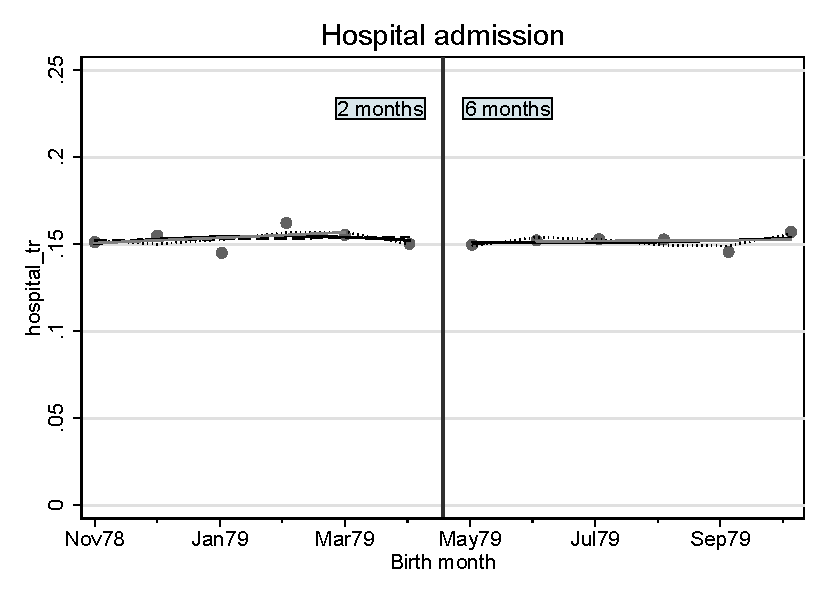
\includegraphics[width=0.99\textwidth]{R1_RD_hospital_tr_fits.pdf}
		\caption{Total}		
	\end{subfigure}
	\begin{subfigure}[t]{0.31\textwidth}
		\centering
		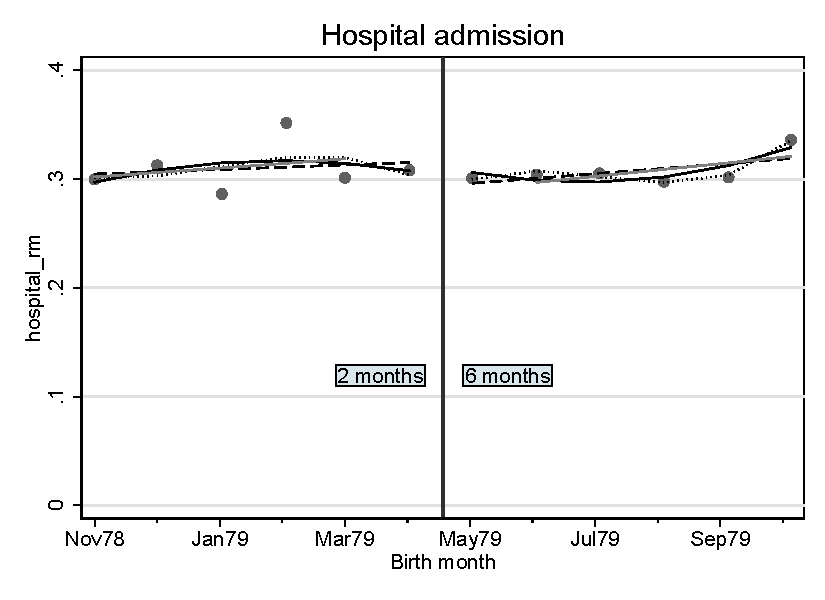
\includegraphics[width=0.99\textwidth]{R1_RD_hospital_rm_fits}
		\caption{Men}		
	\end{subfigure}
	\quad
	\begin{subfigure}[t]{0.31\textwidth}
		\centering
		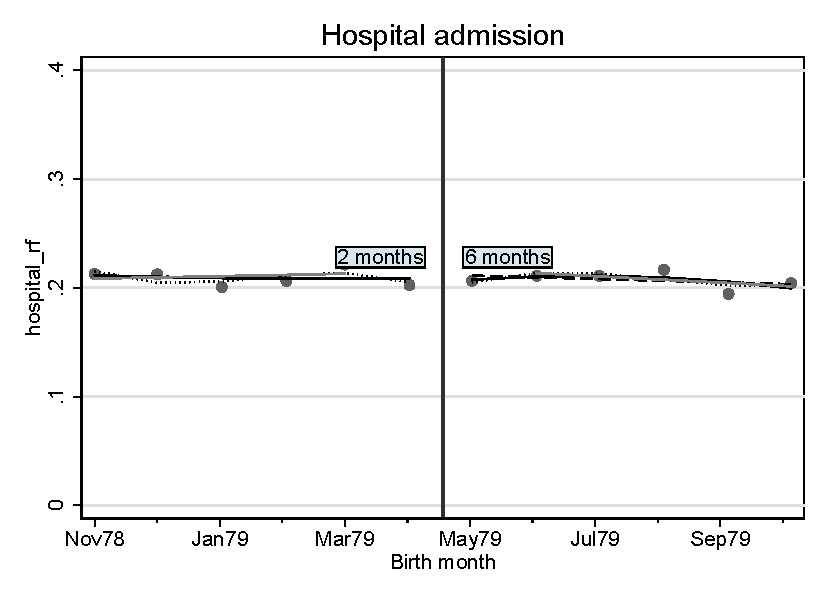
\includegraphics[width=0.99\textwidth]{R1_RD_hospital_rf_fits}
		\caption{Women}
	\end{subfigure}
\end{figure}


\begin{table}[h]\centering
\def\sym#1{\ifmmode^{#1}\else\(^{#1}\)\fi}
\begin{tabular}{l*{3}{c}|cccc}
\toprule
% &\multicolumn{1}{c}{(1)}&\multicolumn{1}{c}{(2)}&\multicolumn{1}{c}{(3)}&\multicolumn{1}{c}{(4)}&\multicolumn{1}{c}{(5)}&\multicolumn{1}{c}{(6)}&\multicolumn{1}{c}{(7)} \\ 
&\multicolumn{3}{c}{bandwidth of 6 months} & \multicolumn{4}{c}{different bandwidths} \\
 \cmidrule(lr{1em}){2-4} \cmidrule(lr{1em}){5-8}
 &\multicolumn{1}{c}{(1)}&\multicolumn{1}{c}{(2)}&\multicolumn{1}{c}{(3)}& 1 Month & 2 Months & 4 Months & 6M \& Donut \\
\midrule 
RD Linear           &    -0.00445         &    -0.00445         &    -0.00445         \\
                    &   (0.00435)         &   (0.00453)         &   (0.00453)         \\
RD Quadratic        &     0.00319         &     0.00319         &     0.00319         \\
                    &   (0.00861)         &   (0.00897)         &   (0.00897)         \\
RD Cubic            &     0.00146         &     0.00146         &     0.00146         \\
                    &    (0.0130)         &    (0.0136)         &    (0.0136)         \\
RD Linear Donut     &    -0.00881         &    -0.00881         &    -0.00881         \\
                    &   (0.00613)         &   (0.00643)         &   (0.00643)         \\
\midrule
DDRD: C1-C3 &    -0.00262         &    -0.00262         &    -0.00262         &     0.00255         &    -0.00137         &    -0.00284         &    -0.00366\sym{*}  \\
            &   (0.00209)         &   (0.00211)         &   (0.00211)         &   (0.00530)         &   (0.00337)         &   (0.00241)         &   (0.00212)         \\
DDRD: C2            &    -0.00452\sym{**} &    -0.00452\sym{**} &    -0.00452\sym{**} &    -0.00795\sym{***}&    -0.00630\sym{***}&    -0.00576\sym{***}&    -0.00383         \\
                    &   (0.00210)         &   (0.00215)         &   (0.00215)         &  (3.32e-17)         &  (0.000946)         &   (0.00177)         &   (0.00245)         \\
DDRD: C1+C2         &    -0.00398\sym{*}  &    -0.00398         &    -0.00398         &   -0.000162         &    -0.00275         &    -0.00472         &    -0.00475\sym{*}  \\
                    &   (0.00233)         &   (0.00236)         &   (0.00236)         &   (0.00496)         &   (0.00375)         &   (0.00278)         &   (0.00239)         \\
Birthmonth FE       &           X         &           X         &           X         &                     &                     &                     &                     \\
Time FE             &                     &           X         &           X         &                     &                     &                     &                     \\
Pers covar          &                     &                     &           X         &                     &                     &                     &                     \\
            &\multicolumn{1}{c}{Men}&\multicolumn{1}{c}{Women}\\
\midrule
DDRD: C1-C3 &    -0.00363         &    -0.00406         \\
            &   (0.00901)         &   (0.00496)         \\
DDRD: C2            &    -0.00823         &    -0.00456         \\
                    &   (0.00915)         &   (0.00486)         \\
DDRD: C1+C2         &     -0.0105         &    -0.00387         \\
                    &    (0.0101)         &   (0.00514)         \\

\bottomrule
\end{tabular}
\end{table}


\begin{figure}[h!]
	\centering
	\begin{subfigure}[t]{0.31\textwidth}
		\centering
		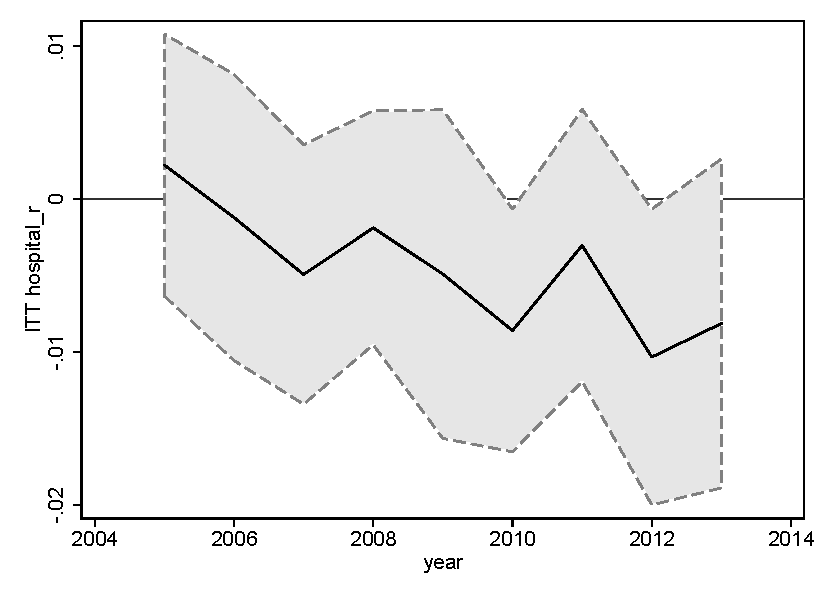
\includegraphics[width=0.99\textwidth]{R1_LC_hospital_r}
		\caption{Total}		
	\end{subfigure}
	\begin{subfigure}[t]{0.31\textwidth}
		\centering
		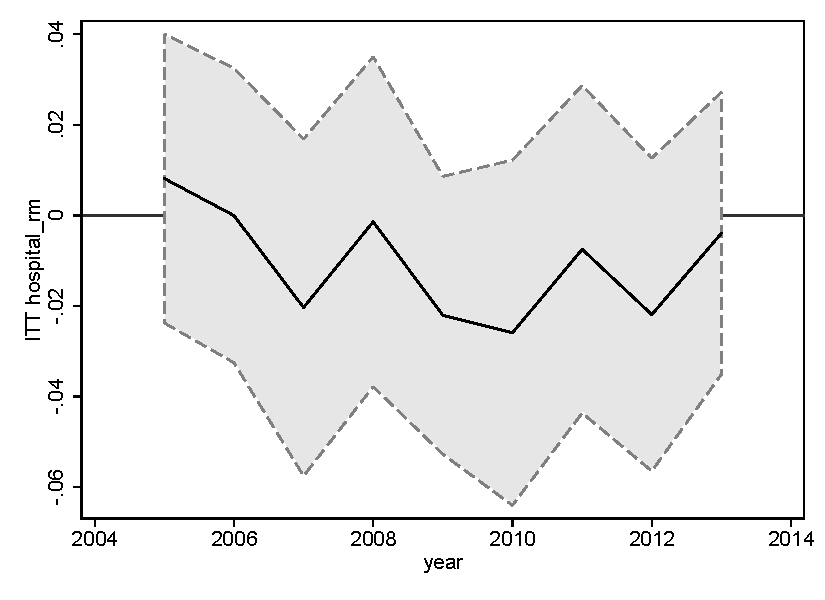
\includegraphics[width=0.99\textwidth]{R1_LC_hospital_rm}
		\caption{Men}		
	\end{subfigure}
	\quad
	\begin{subfigure}[t]{0.31\textwidth}
		\centering
		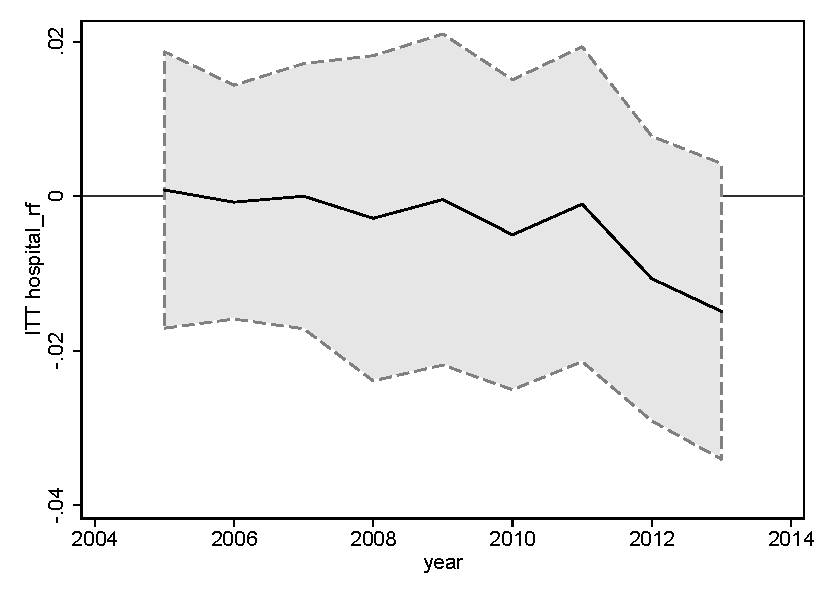
\includegraphics[width=0.99\textwidth]{R1_LC_hospital_rf}
		\caption{Women}
	\end{subfigure}
\end{figure}

%------------------------------------------------------------------------------------
\newpage
\begin{figure}[h]
	\centering
	\begin{subfigure}[t]{0.31\textwidth}
		\centering
		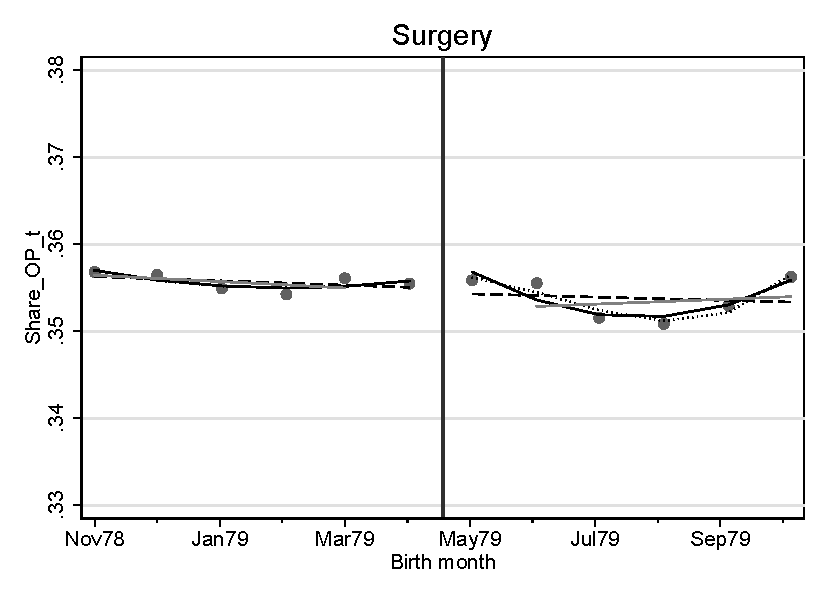
\includegraphics[width=0.99\textwidth]{R1_RD_Share_OP_t_fits}
		\caption{Total}		
	\end{subfigure}
	\begin{subfigure}[t]{0.31\textwidth}
		\centering
		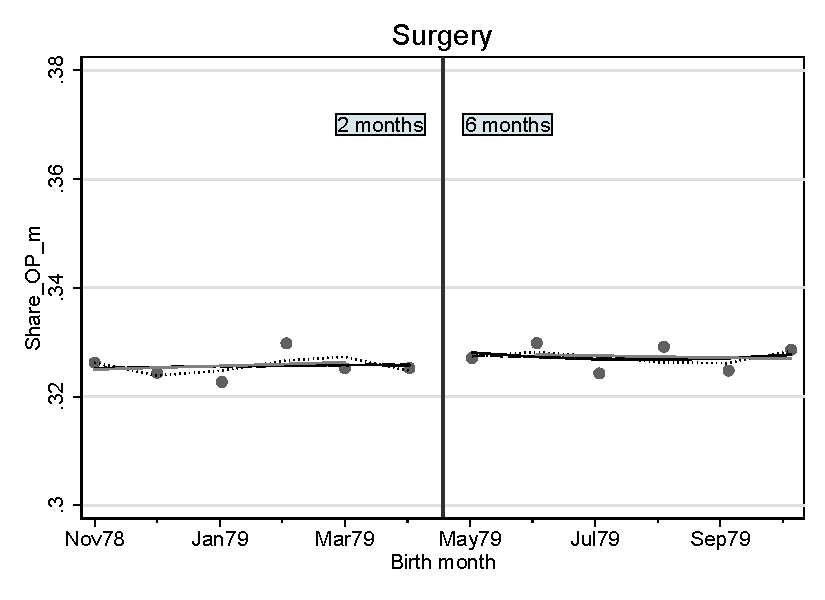
\includegraphics[width=0.99\textwidth]{R1_RD_Share_OP_m_fits}
		\caption{Men}		
	\end{subfigure}
	\quad
	\begin{subfigure}[t]{0.31\textwidth}
		\centering
		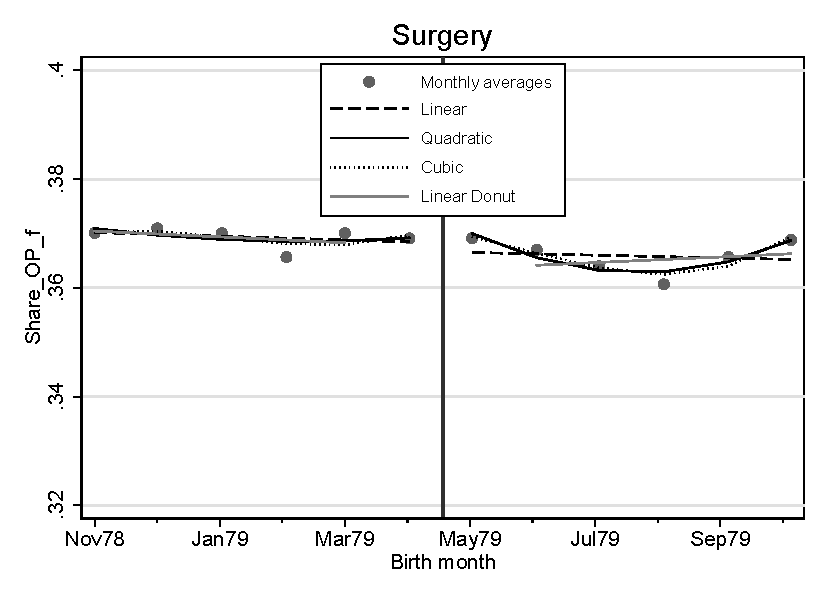
\includegraphics[width=0.99\textwidth]{R1_RD_Share_OP_f_fits}
		\caption{Women}
	\end{subfigure}
\end{figure}


\begin{table}[h]\centering
\def\sym#1{\ifmmode^{#1}\else\(^{#1}\)\fi}
\begin{tabular}{l*{3}{c}|cccc}
\toprule
&\multicolumn{3}{c}{bandwidth of 6 months} & \multicolumn{4}{c}{different bandwidths} \\
 \cmidrule(lr{1em}){2-4} \cmidrule(lr{1em}){5-8}
 &\multicolumn{1}{c}{(1)}&\multicolumn{1}{c}{(2)}&\multicolumn{1}{c}{(3)}& 1 Month & 2 Months & 4 Months & 6M \& Donut \\
\midrule 
RD Linear           &   -0.000334         &   -0.000334         &   -0.000334         \\
                    &   (0.00191)         &   (0.00199)         &   (0.00199)         \\
RD Quadratic        &     0.00470\sym{**} &     0.00470\sym{**} &     0.00470\sym{**} \\
                    &   (0.00191)         &   (0.00199)         &   (0.00199)         \\
RD Cubic            &   -0.000369         &   -0.000369         &   -0.000369         \\
                    &   (0.00319)         &   (0.00332)         &   (0.00332)         \\
RD Linear Donut     &    -0.00194         &    -0.00194         &    -0.00194         \\
                    &   (0.00369)         &   (0.00388)         &   (0.00388)         \\
\midrule
DDRD: C1-C3 &     0.00120         &     0.00120         &     0.00120         &     0.00312         &     0.00318         &     0.00104         &    0.000810         \\
            &   (0.00199)         &   (0.00201)         &   (0.00201)         &   (0.00484)         &   (0.00342)         &   (0.00257)         &   (0.00219)         \\
DDRD: C2            &    0.000179         &    0.000179         &    0.000179         &     0.00266\sym{***}&     0.00123         &    0.000197         &   -0.000316         \\
                    &  (0.000693)         &  (0.000707)         &  (0.000707)         &  (3.49e-17)         &  (0.000813)         &  (0.000811)         &  (0.000761)         \\
DDRD: C1+C2         &    0.000744         &    0.000744         &    0.000744         &     0.00319         &     0.00246\sym{*}  &    0.000687         &    0.000255         \\
                    &   (0.00120)         &   (0.00121)         &   (0.00121)         &   (0.00187)         &   (0.00121)         &   (0.00162)         &   (0.00136)         \\
Birthmonth FE       &           X         &           X         &           X         &                     &                     &                     &                     \\
Time FE             &                     &           X         &           X         &                     &                     &                     &                     \\
Pers covar          &                     &                     &           X         &                     &                     &                     &                     \\
            &\multicolumn{1}{c}{Men}&\multicolumn{1}{c}{Women}\\
\midrule
DDRD: C1-C3 &     0.00366\sym{**} &  -0.0000107         \\
            &   (0.00143)         &   (0.00305)         \\
DDRD: C2            &     0.00471\sym{***}&    -0.00117         \\
                    &   (0.00112)         &   (0.00185)         \\
DDRD: C1+C2         &     0.00354\sym{***}&    -0.00155         \\
                    &  (0.000794)         &   (0.00121)         \\

\bottomrule
\end{tabular}
\end{table}


\begin{figure}[h!]
	\centering
	\begin{subfigure}[t]{0.31\textwidth}
		\centering
		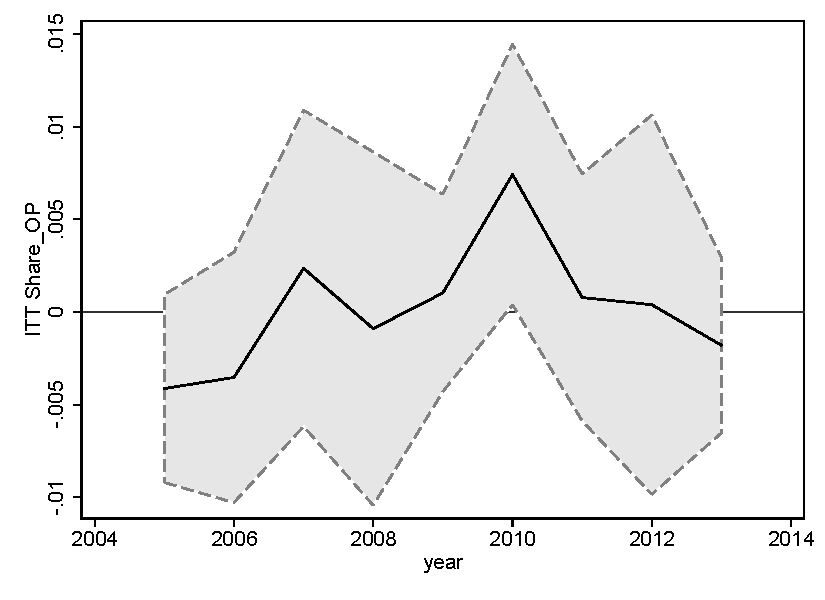
\includegraphics[width=0.99\textwidth]{R1_LC_Share_OP}
		\caption{Total}		
	\end{subfigure}
	\begin{subfigure}[t]{0.31\textwidth}
		\centering
		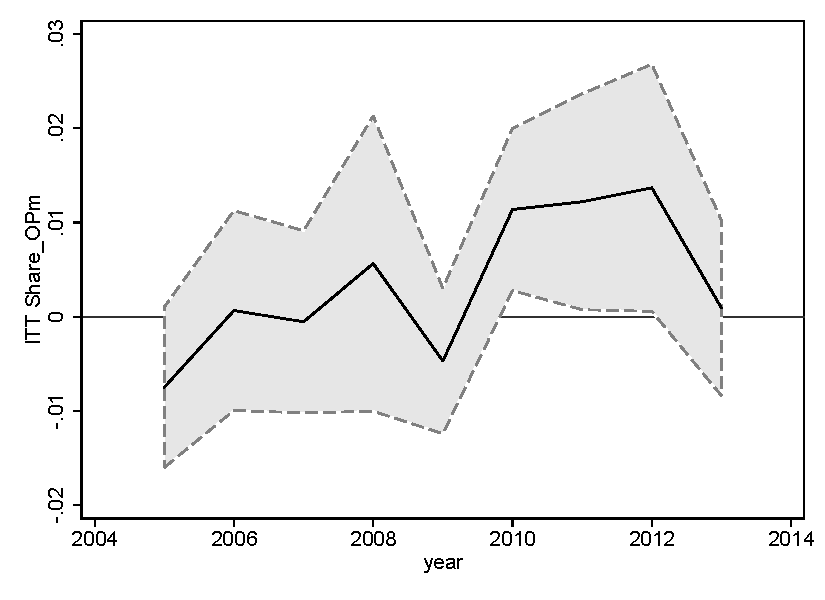
\includegraphics[width=0.99\textwidth]{R1_LC_Share_OPm}
		\caption{Men}		
	\end{subfigure}
	\quad
	\begin{subfigure}[t]{0.31\textwidth}
		\centering
		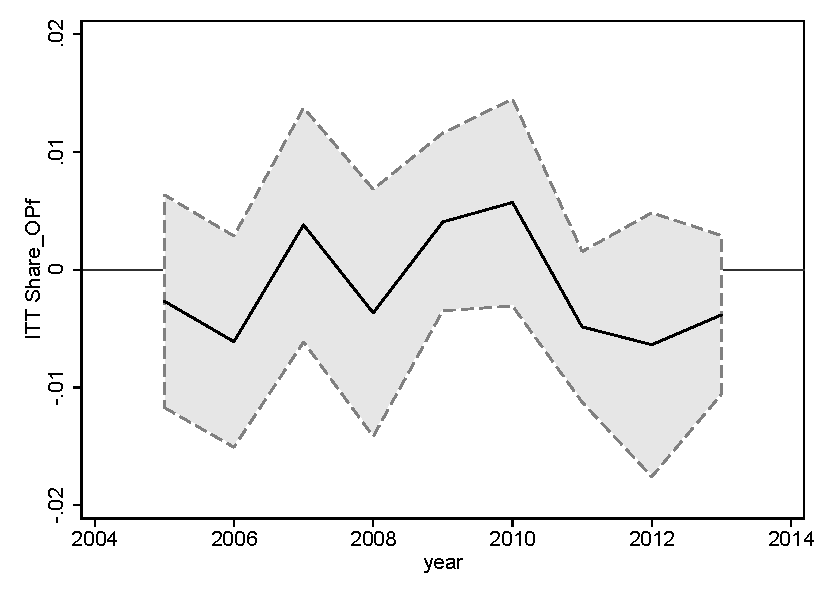
\includegraphics[width=0.99\textwidth]{R1_LC_Share_OPf}
		\caption{Women}
	\end{subfigure}
\end{figure}
%------------------------------------------------------------------------------------
\newpage
\begin{figure}[h]
	\centering
	\begin{subfigure}[t]{0.31\textwidth}
		\centering
		\includegraphics[width=0.99\textwidth]{R1_RD_LOS_fits}
		\caption{Total}		
	\end{subfigure}
	\begin{subfigure}[t]{0.31\textwidth}
		\centering
		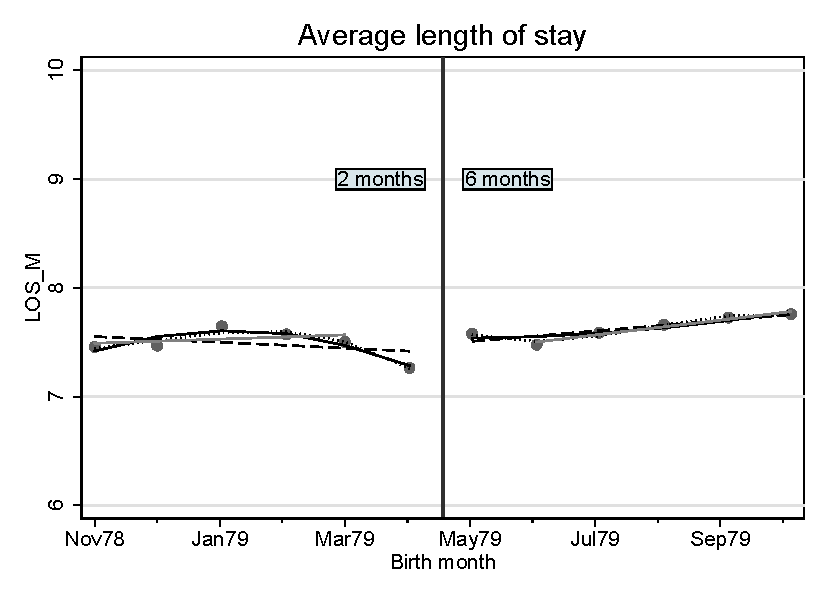
\includegraphics[width=0.99\textwidth]{R1_RD_LOS_M_fits}
		\caption{Men}		
	\end{subfigure}
	\quad
	\begin{subfigure}[t]{0.31\textwidth}
		\centering
		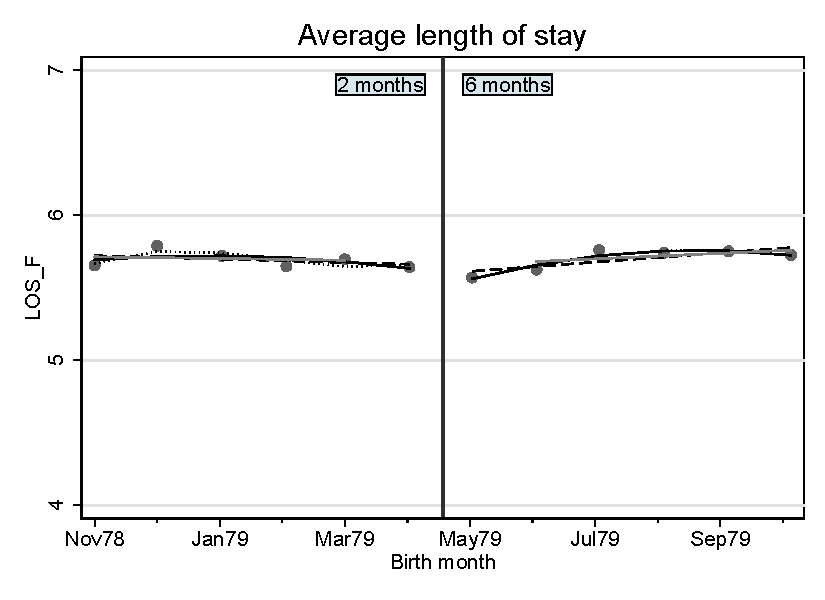
\includegraphics[width=0.99\textwidth]{R1_RD_LOS_F_fits}
		\caption{Women}
	\end{subfigure}
\end{figure}


\begin{table}[h]\centering
\def\sym#1{\ifmmode^{#1}\else\(^{#1}\)\fi}
\begin{tabular}{l*{3}{c}|cccc}
\toprule
 &\multicolumn{1}{c}{(1)}&\multicolumn{1}{c}{(2)}&\multicolumn{1}{c}{(3)}\\  
\midrule 
RD Linear           &     -0.0343         &     -0.0343         &     -0.0343         \\
                    &    (0.0673)         &    (0.0700)         &    (0.0700)         \\
RD Quadratic        &      0.0992\sym{*}  &      0.0992\sym{*}  &      0.0992\sym{*}  \\
                    &    (0.0477)         &    (0.0497)         &    (0.0497)         \\
RD Cubic            &       0.120         &       0.120         &       0.120         \\
                    &     (0.108)         &     (0.113)         &     (0.113)         \\
RD Linear Donut     &      -0.130         &      -0.130         &      -0.130         \\
                    &    (0.0819)         &    (0.0860)         &    (0.0860)         \\
\midrule
DDRD: C1-C3 &      0.0526         &      0.0526         &      0.0526         &      0.0458         &    -0.00370         &      0.0255         &      0.0539\sym{*}  \\
            &    (0.0334)         &    (0.0337)         &    (0.0337)         &    (0.0373)         &    (0.0405)         &    (0.0450)         &    (0.0296)         \\
DDRD: C2            &      0.0503\sym{*}  &      0.0503         &      0.0503         &       0.103\sym{***}&      0.0308         &     0.00349         &      0.0398         \\
                    &    (0.0293)         &    (0.0299)         &    (0.0299)         &  (5.96e-16)         &    (0.0323)         &    (0.0330)         &    (0.0285)         \\
DDRD: C1+C2         &      0.0623\sym{*}  &      0.0623\sym{*}  &      0.0623\sym{*}  &      0.0480         &      0.0106         &      0.0319         &      0.0651\sym{**} \\
                    &    (0.0317)         &    (0.0321)         &    (0.0321)         &    (0.0558)         &    (0.0395)         &    (0.0406)         &    (0.0282)         \\
Birthmonth FE       &           X         &           X         &           X         &                     &                     &                     &                     \\
Time FE             &                     &           X         &           X         &                     &                     &                     &                     \\
Pers covar          &                     &                     &           X         &                     &                     &                     &                     \\
            &\multicolumn{1}{c}{Men}&\multicolumn{1}{c}{Women}\\
\midrule
DDRD: C1-C3 &       0.107\sym{*}  &      0.0325         \\
            &    (0.0583)         &    (0.0344)         \\
DDRD: C2            &      0.0818         &      0.0579\sym{*}  \\
                    &    (0.0622)         &    (0.0327)         \\
DDRD: C1+C2         &      0.0900         &      0.0383         \\
                    &    (0.0653)         &    (0.0234)         \\

\bottomrule
\end{tabular}
\end{table}


\begin{figure}[h!]
	\centering
	\begin{subfigure}[t]{0.31\textwidth}
		\centering
		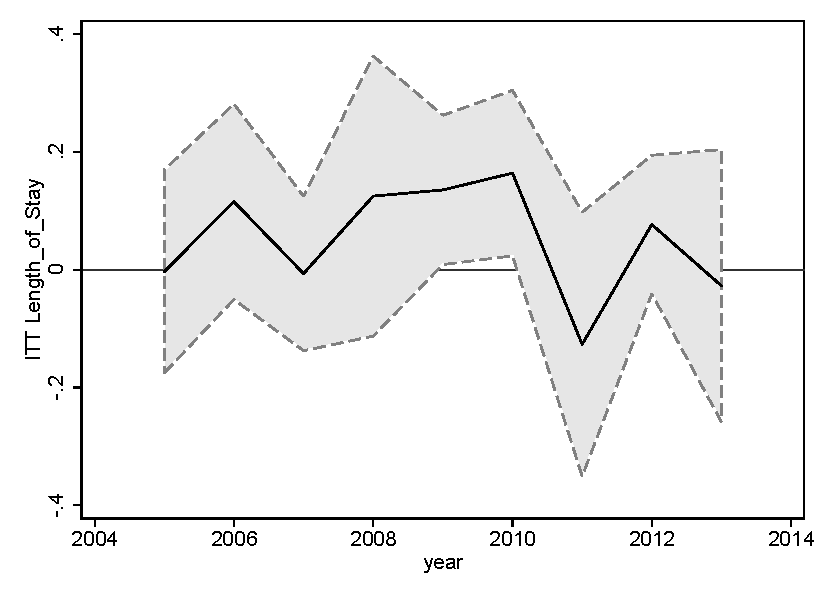
\includegraphics[width=0.99\textwidth]{R1_LC_Length_of_Stay}
		\caption{Total}		
	\end{subfigure}
	\begin{subfigure}[t]{0.31\textwidth}
		\centering
		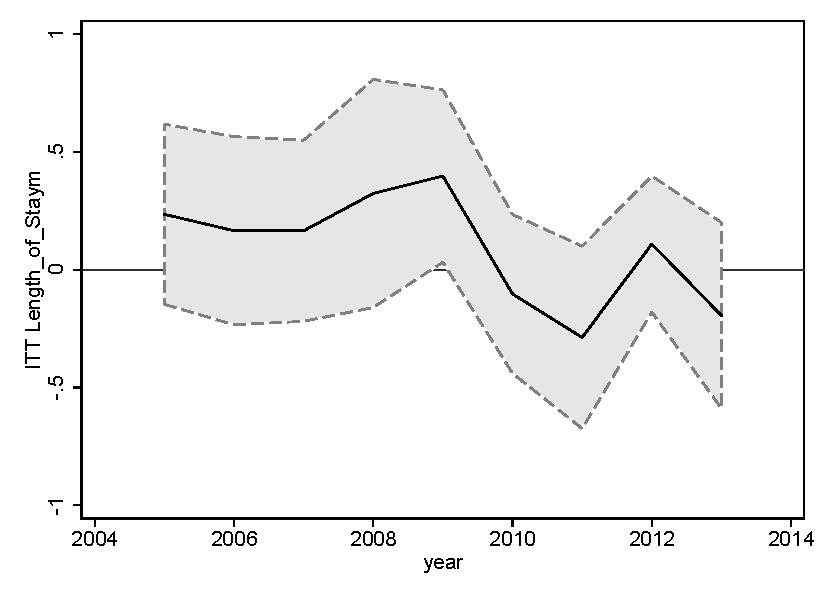
\includegraphics[width=0.99\textwidth]{R1_LC_Length_of_Staym}
		\caption{Men}		
	\end{subfigure}
	\quad
	\begin{subfigure}[t]{0.31\textwidth}
		\centering
		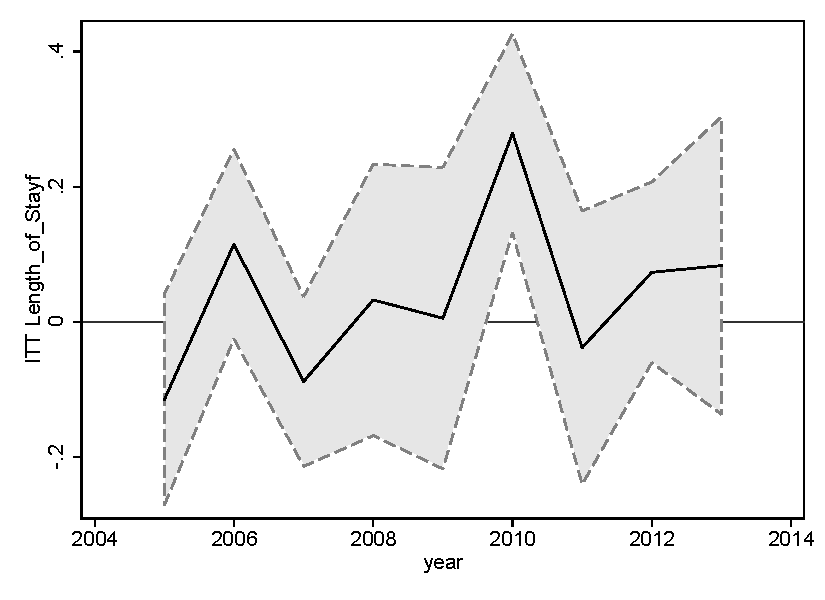
\includegraphics[width=0.99\textwidth]{R1_LC_Length_of_Stayf}
		\caption{Women}
	\end{subfigure}
\end{figure}

%
%%------------------------------------------------------------------------------------
\newpage
\section{Hauptdiagnose Kapitel}

\begin{figure}[h]
	\centering
	\begin{subfigure}[t]{0.31\textwidth}
		\centering
		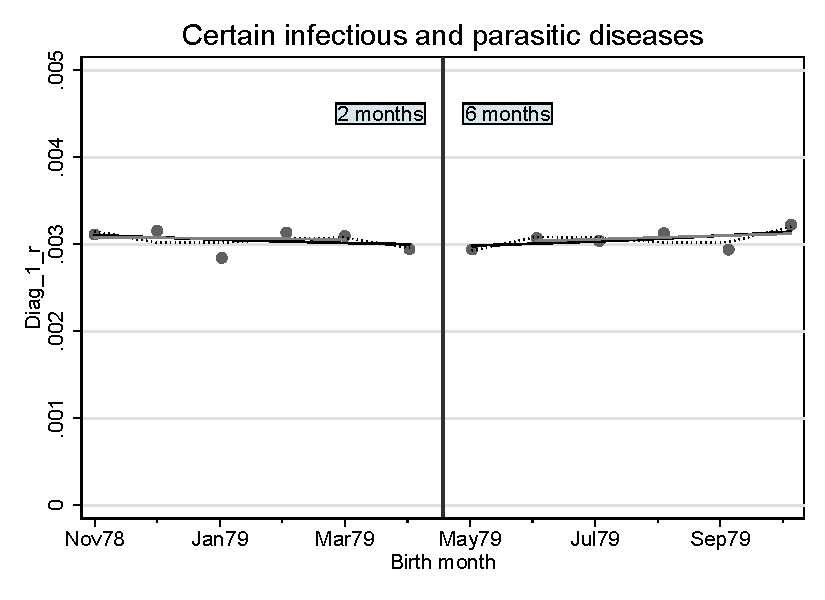
\includegraphics[width=0.99\textwidth]{R1_RD_Diag_1_r_fits}
		\caption{Total}		
	\end{subfigure}
	\begin{subfigure}[t]{0.31\textwidth}
		\centering
		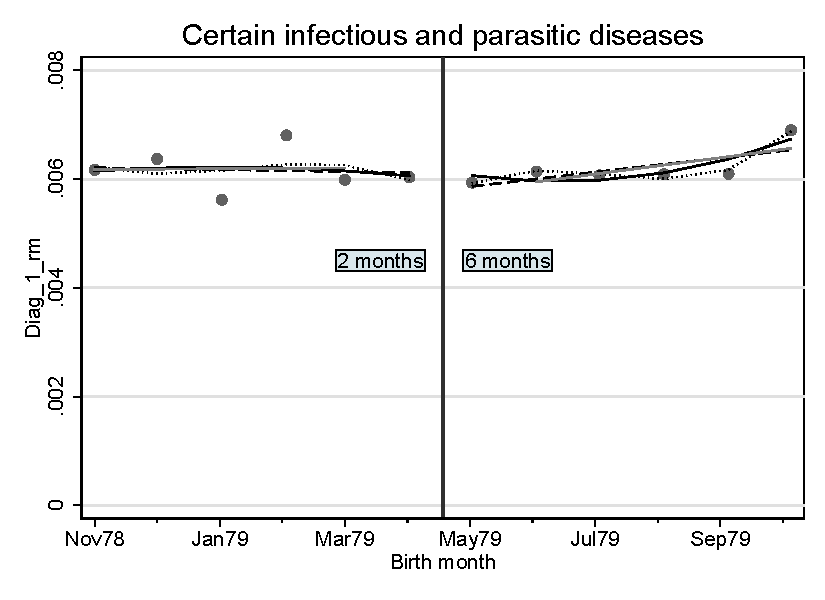
\includegraphics[width=0.99\textwidth]{R1_RD_Diag_1_rm_fits}
		\caption{Men}		
	\end{subfigure}
	\quad
	\begin{subfigure}[t]{0.31\textwidth}
		\centering
		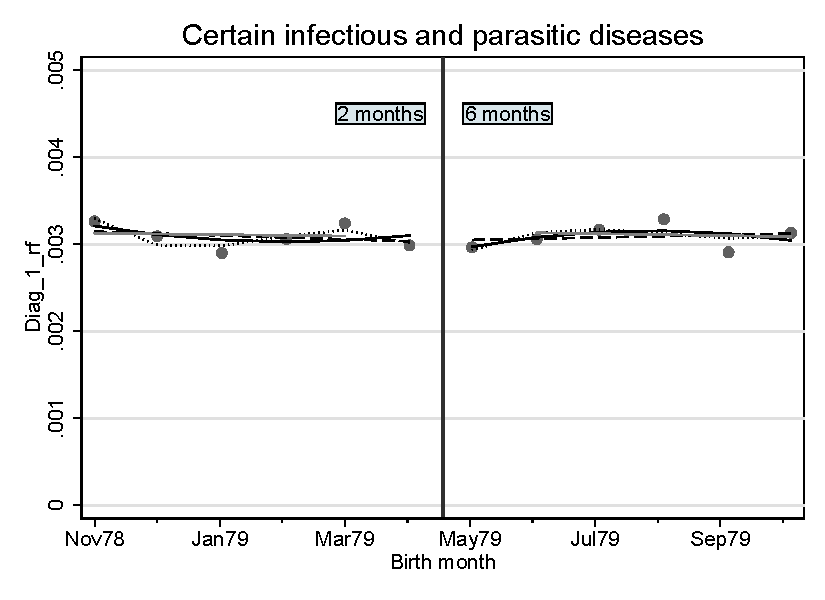
\includegraphics[width=0.99\textwidth]{R1_RD_Diag_1_rf_fits}
		\caption{Women}
	\end{subfigure}
\end{figure}

\begin{table}[h]\centering
\def\sym#1{\ifmmode^{#1}\else\(^{#1}\)\fi}
\begin{tabular}{l*{3}{c}|cccc}
\toprule
&\multicolumn{3}{c}{bandwidth of 6 months} & \multicolumn{4}{c}{different bandwidths} \\
 \cmidrule(lr{1em}){2-4} \cmidrule(lr{1em}){5-8}
 &\multicolumn{1}{c}{(1)}&\multicolumn{1}{c}{(2)}&\multicolumn{1}{c}{(3)}& 1 Month & 2 Months & 4 Months & 6M \& Donut \\
\midrule 
RD Linear           &  -0.0000286         &  -0.0000286         &  -0.0000286         \\
                    & (0.0000841)         & (0.0000875)         & (0.0000875)         \\
RD Quadratic        &  -0.0000235         &  -0.0000235         &  -0.0000235         \\
                    &  (0.000205)         &  (0.000213)         &  (0.000213)         \\
RD Cubic            &   -0.000121         &   -0.000121         &   -0.000121         \\
                    &  (0.000282)         &  (0.000294)         &  (0.000294)         \\
RD Linear Donut     &  -0.0000482         &  -0.0000482         &  -0.0000482         \\
                    &  (0.000118)         &  (0.000124)         &  (0.000124)         \\
\midrule
DDRD: C1-C3 &  -0.0000264         &  -0.0000264         &  -0.0000264         &  -0.0000315         &  -0.0000860         &  0.00000972         &  -0.0000253         \\
            & (0.0000512)         & (0.0000517)         & (0.0000517)         &  (0.000113)         & (0.0000811)         & (0.0000640)         & (0.0000553)         \\
DDRD: C2            &  -0.0000687         &  -0.0000687         &  -0.0000687         &   -0.000365\sym{***}&   -0.000280\sym{***}&  -0.0000664         & -0.00000941         \\
                    & (0.0000603)         & (0.0000615)         & (0.0000615)         &  (5.37e-19)         & (0.0000422)         & (0.0000712)         & (0.0000640)         \\
DDRD: C1+C2         &  -0.0000703         &  -0.0000703         &  -0.0000703         &   -0.000124         &   -0.000160         &  -0.0000477         &  -0.0000596         \\
                    & (0.0000561)         & (0.0000569)         & (0.0000569)         &  (0.000150)         & (0.0000976)         & (0.0000708)         & (0.0000584)         \\
Birthmonth FE       &           X         &           X         &           X         &                     &                     &                     &                     \\
Time FE             &                     &           X         &           X         &                     &                     &                     &                     \\
Pers covar          &                     &                     &           X         &                     &                     &                     &                     \\
            &\multicolumn{1}{c}{Men}&\multicolumn{1}{c}{Women}\\
\midrule
DDRD: C1-C3 & -0.00000909         &  -0.0000144         \\
            &  (0.000168)         & (0.0000905)         \\
DDRD: C2            &   -0.000133         &  -0.0000465         \\
                    &  (0.000168)         & (0.0000954)         \\
DDRD: C1+C2         &   -0.000148         &  -0.0000365         \\
                    &  (0.000196)         & (0.0000998)         \\

\bottomrule
\end{tabular}
\end{table}


\begin{figure}[h!]
	\centering
	\begin{subfigure}[t]{0.31\textwidth}
		\centering
		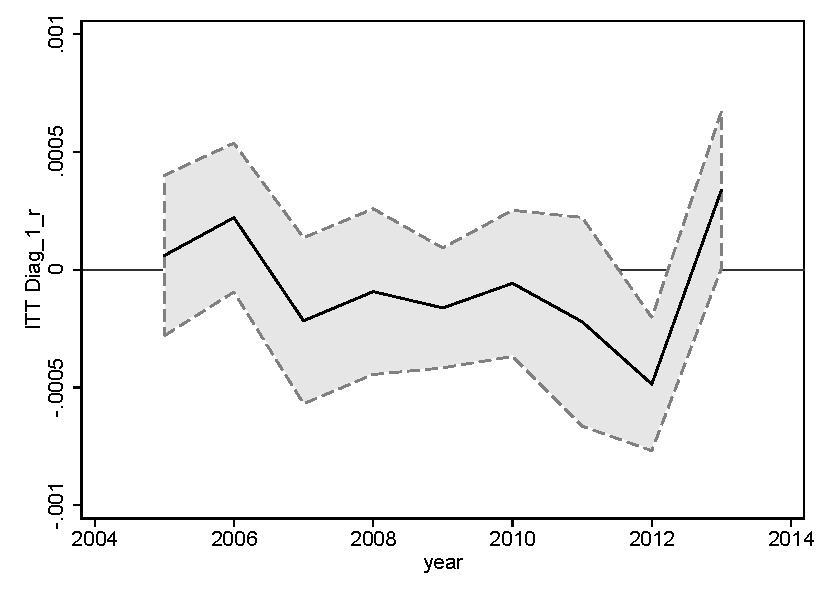
\includegraphics[width=0.99\textwidth]{R1_LC_Diag_1_r}
		\caption{Total}		
	\end{subfigure}
	\begin{subfigure}[t]{0.31\textwidth}
		\centering
		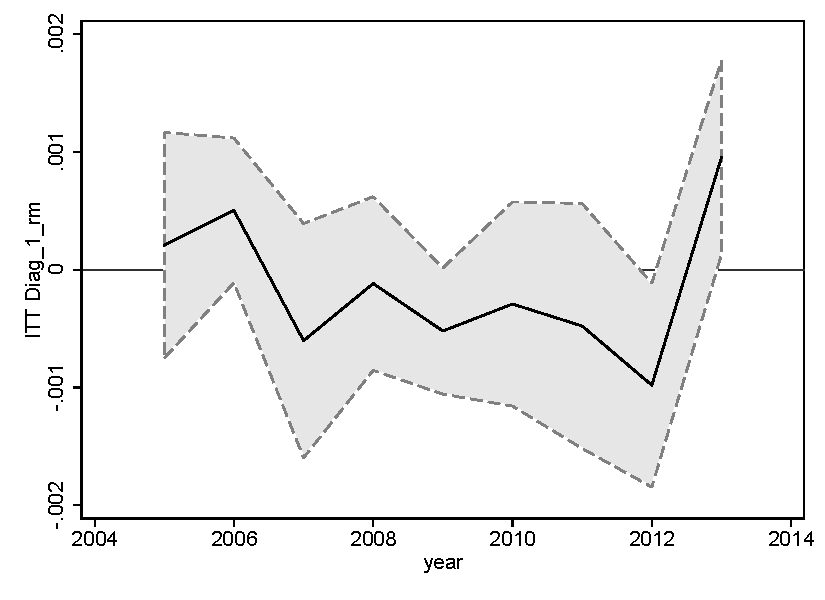
\includegraphics[width=0.99\textwidth]{R1_LC_Diag_1_rm}
		\caption{Men}		
	\end{subfigure}
	\quad
	\begin{subfigure}[t]{0.31\textwidth}
		\centering
		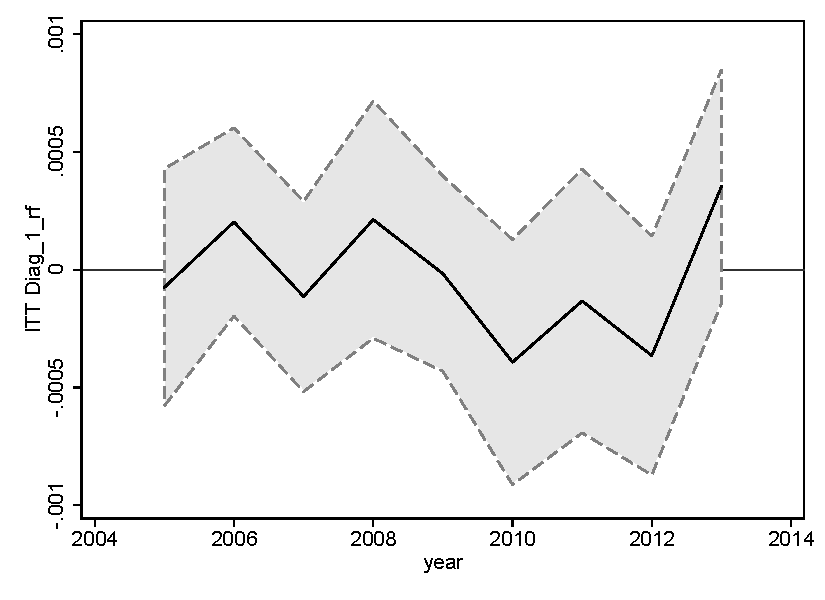
\includegraphics[width=0.99\textwidth]{R1_LC_Diag_1_rf}
		\caption{Women}
	\end{subfigure}
\end{figure}
%%------------------------------------------------------------------------------------
\newpage
\begin{figure}[h]
	\centering
	\begin{subfigure}[t]{0.31\textwidth}
		\centering
		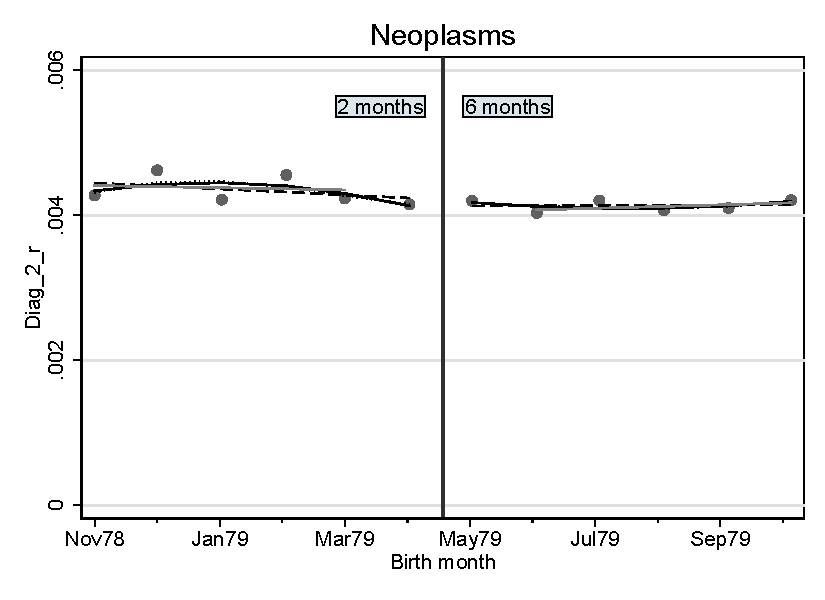
\includegraphics[width=0.99\textwidth]{R1_RD_Diag_2_r_fits}
		\caption{Total}		
	\end{subfigure}
	\begin{subfigure}[t]{0.31\textwidth}
		\centering
		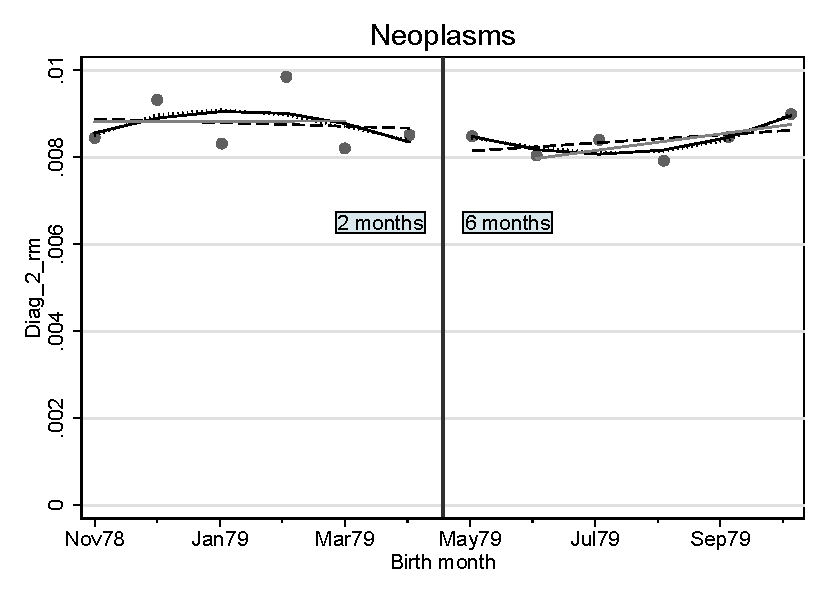
\includegraphics[width=0.99\textwidth]{R1_RD_Diag_2_rm_fits}
		\caption{Men}		
	\end{subfigure}
	\quad
	\begin{subfigure}[t]{0.31\textwidth}
		\centering
		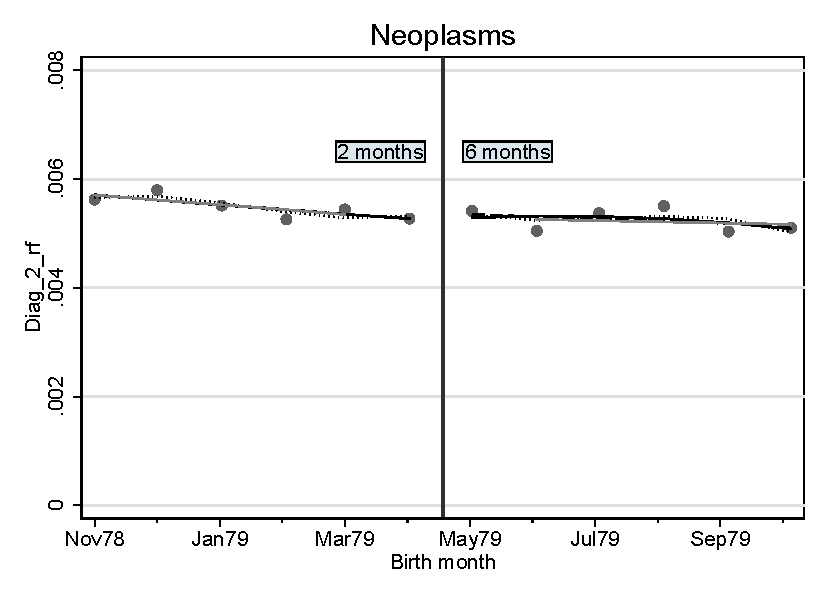
\includegraphics[width=0.99\textwidth]{R1_RD_Diag_2_rf_fits}
		\caption{Women}
	\end{subfigure}
\end{figure}


\begin{table}[h]\centering
\def\sym#1{\ifmmode^{#1}\else\(^{#1}\)\fi}
\begin{tabular}{l*{3}{c}|cccc}
\toprule
&\multicolumn{3}{c}{bandwidth of 6 months} & \multicolumn{4}{c}{different bandwidths} \\
 \cmidrule(lr{1em}){2-4} \cmidrule(lr{1em}){5-8}
 &\multicolumn{1}{c}{(1)}&\multicolumn{1}{c}{(2)}&\multicolumn{1}{c}{(3)}& 1 Month & 2 Months & 4 Months & 6M \& Donut \\
\midrule 
RD Linear           &  -0.0000717         &  -0.0000717         &  -0.0000717         \\
                    &  (0.000139)         &  (0.000144)         &  (0.000144)         \\
RD Quadratic        &    0.000363\sym{*}  &    0.000363\sym{*}  &    0.000363\sym{*}  \\
                    &  (0.000194)         &  (0.000202)         &  (0.000202)         \\
RD Cubic            &    0.000168         &    0.000168         &    0.000168         \\
                    &  (0.000417)         &  (0.000435)         &  (0.000435)         \\
RD Linear Donut     &   -0.000294         &   -0.000294         &   -0.000294         \\
                    &  (0.000222)         &  (0.000233)         &  (0.000233)         \\
\midrule
DDRD: C1-C3 &  -0.0000736         &  -0.0000736         &  -0.0000736         &    0.000226         &   0.0000106         &  -0.0000823         &   -0.000134         \\
            &  (0.000169)         &  (0.000171)         &  (0.000171)         &  (0.000401)         &  (0.000258)         &  (0.000186)         &  (0.000183)         \\
DDRD: C2            &  -0.0000676         &  -0.0000676         &  -0.0000676         &   -0.000137\sym{***}&   -0.000112\sym{***}&   -0.000128         &  -0.0000536         \\
                    & (0.0000837)         & (0.0000854)         & (0.0000854)         &  (1.39e-18)         & (0.0000185)         & (0.0000773)         & (0.0000901)         \\
DDRD: C1+C2         &  -0.0000835         &  -0.0000835         &  -0.0000835         &    0.000163         &  0.00000696         &   -0.000130         &   -0.000133         \\
                    &  (0.000117)         &  (0.000119)         &  (0.000119)         &  (0.000218)         &  (0.000132)         &  (0.000120)         &  (0.000129)         \\
Birthmonth FE       &           X         &           X         &           X         &                     &                     &                     &                     \\
Time FE             &                     &           X         &           X         &                     &                     &                     &                     \\
Pers covar          &                     &                     &           X         &                     &                     &                     &                     \\
            &\multicolumn{1}{c}{Men}&\multicolumn{1}{c}{Women}\\
\midrule
DDRD: C1-C3 &  -0.0000999         &   0.0000715         \\
            &  (0.000424)         &  (0.000282)         \\
DDRD: C2            &   -0.000167         &    0.000106         \\
                    &  (0.000346)         &  (0.000204)         \\
DDRD: C1+C2         &   -0.000160         &   0.0000867         \\
                    &  (0.000322)         &  (0.000162)         \\

\bottomrule
\end{tabular}
\end{table}


\begin{figure}[h!]
	\centering
	\begin{subfigure}[t]{0.31\textwidth}
		\centering
		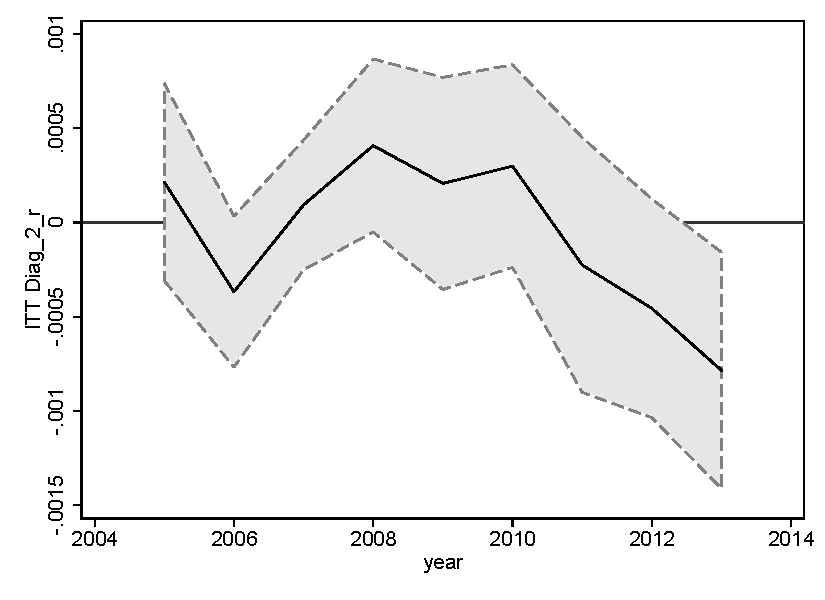
\includegraphics[width=0.99\textwidth]{R1_LC_Diag_2_r}
		\caption{Total}		
	\end{subfigure}
	\begin{subfigure}[t]{0.31\textwidth}
		\centering
		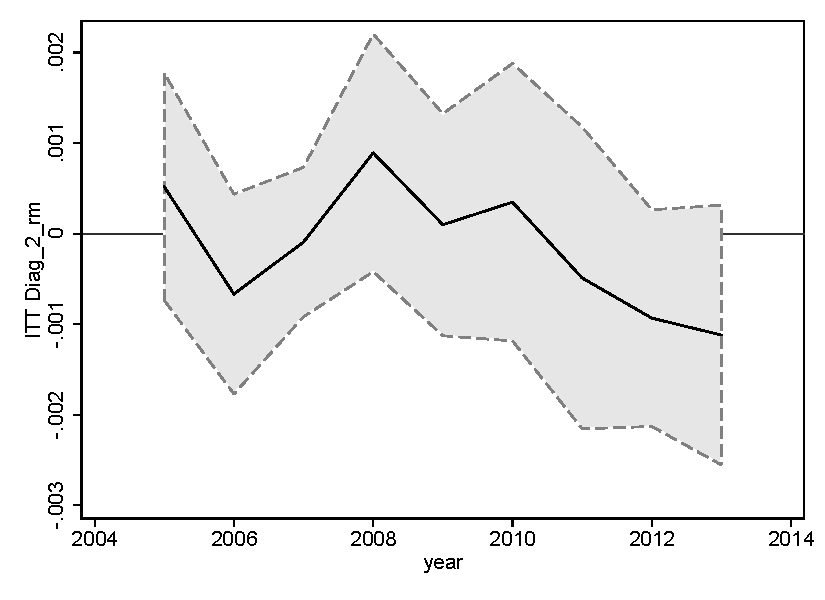
\includegraphics[width=0.99\textwidth]{R1_LC_Diag_2_rm}
		\caption{Men}		
	\end{subfigure}
	\quad
	\begin{subfigure}[t]{0.31\textwidth}
		\centering
		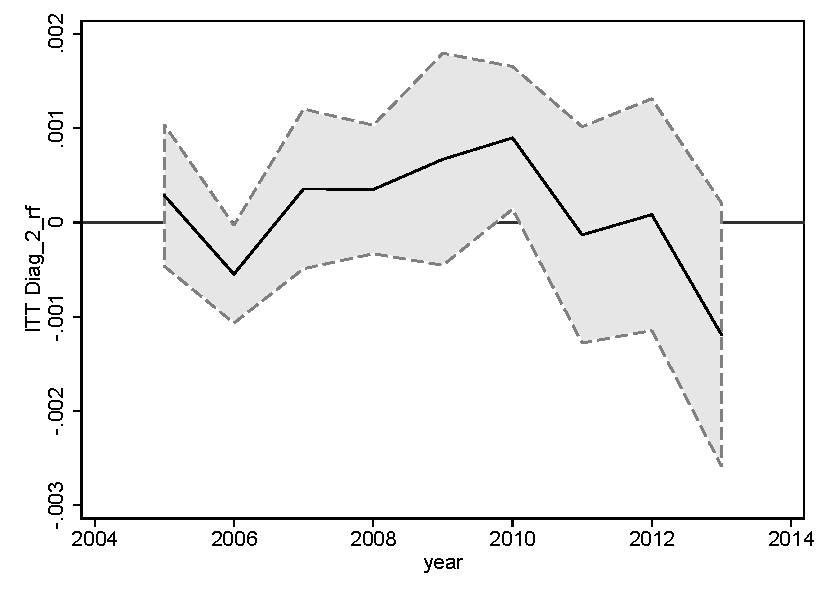
\includegraphics[width=0.99\textwidth]{R1_LC_Diag_2_rf}
		\caption{Women}
	\end{subfigure}
\end{figure}
%%------------------------------------------------------------------------------------
\newpage
\begin{figure}[h]
	\centering
	\begin{subfigure}[t]{0.31\textwidth}
		\centering
		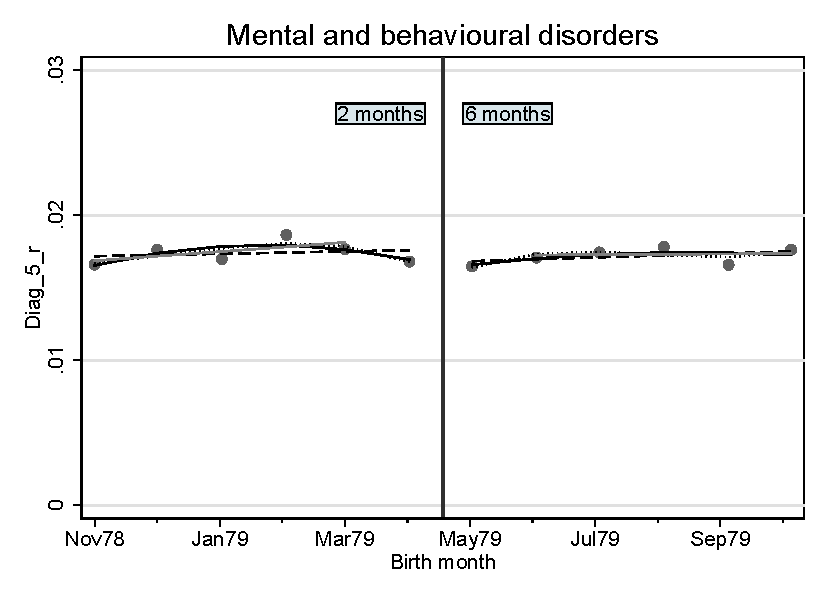
\includegraphics[width=0.99\textwidth]{R1_RD_Diag_5_r_fits}
		\caption{Total}		
	\end{subfigure}
	\begin{subfigure}[t]{0.31\textwidth}
		\centering
		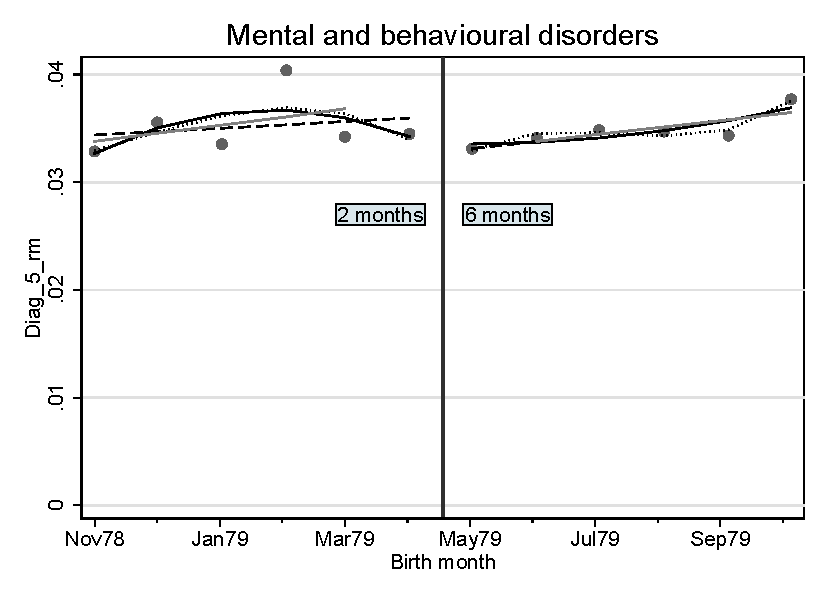
\includegraphics[width=0.99\textwidth]{R1_RD_Diag_5_rm_fits}
		\caption{Men}		
	\end{subfigure}
	\quad
	\begin{subfigure}[t]{0.31\textwidth}
		\centering
		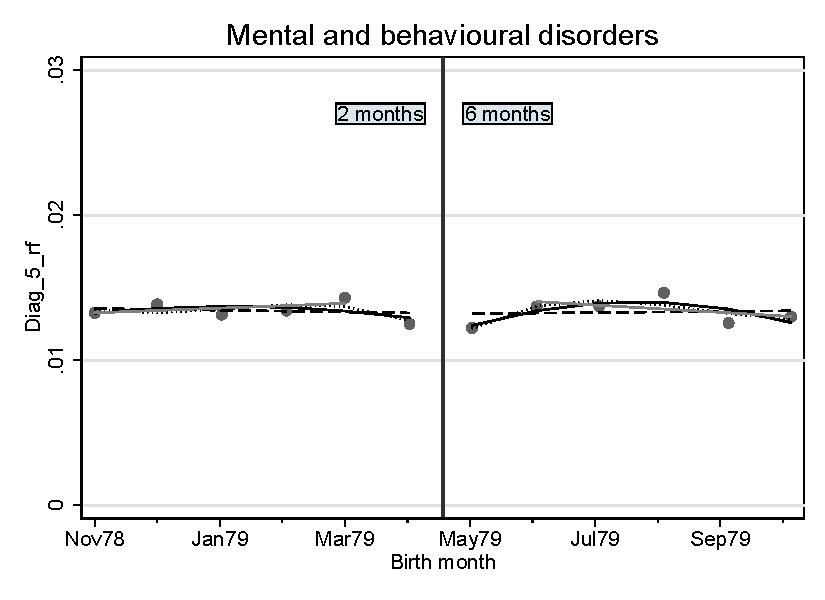
\includegraphics[width=0.99\textwidth]{R1_RD_Diag_5_rf_fits}
		\caption{Women}
	\end{subfigure}
\end{figure}


\begin{table}[h]\centering
\def\sym#1{\ifmmode^{#1}\else\(^{#1}\)\fi}
\begin{tabular}{l*{3}{c}|cccc}
\toprule
&\multicolumn{3}{c}{bandwidth of 6 months} & \multicolumn{4}{c}{different bandwidths} \\
 \cmidrule(lr{1em}){2-4} \cmidrule(lr{1em}){5-8}
 &\multicolumn{1}{c}{(1)}&\multicolumn{1}{c}{(2)}&\multicolumn{1}{c}{(3)}& 1 Month & 2 Months & 4 Months & 6M \& Donut \\
\midrule 
RD Linear           &   -0.000973         &   -0.000973         &   -0.000973         \\
                    &  (0.000756)         &  (0.000787)         &  (0.000787)         \\
RD Quadratic        &    0.000137         &    0.000137         &    0.000137         \\
                    &  (0.000820)         &  (0.000854)         &  (0.000854)         \\
RD Cubic            &   -0.000297         &   -0.000297         &   -0.000297         \\
                    &   (0.00146)         &   (0.00152)         &   (0.00152)         \\
RD Linear Donut     &    -0.00156\sym{*}  &    -0.00156         &    -0.00156         \\
                    &  (0.000838)         &  (0.000880)         &  (0.000880)         \\
\midrule
DDRD: C1-C3 &   -0.000583         &   -0.000583         &   -0.000583         &   -0.000383         &   -0.000748         &   -0.000772\sym{*}  &   -0.000623         \\
            &  (0.000348)         &  (0.000351)         &  (0.000351)         &  (0.000584)         &  (0.000482)         &  (0.000396)         &  (0.000377)         \\
DDRD: C2            &    -0.00105\sym{***}&    -0.00105\sym{**} &    -0.00105\sym{**} &    -0.00164\sym{***}&    -0.00132\sym{***}&    -0.00157\sym{***}&   -0.000933\sym{**} \\
                    &  (0.000371)         &  (0.000378)         &  (0.000378)         &  (1.23e-18)         &  (0.000192)         &  (0.000244)         &  (0.000435)         \\
DDRD: C1+C2         &   -0.000806\sym{**} &   -0.000806\sym{*}  &   -0.000806\sym{*}  &   -0.000704         &   -0.000789         &    -0.00106\sym{**} &   -0.000826\sym{*}  \\
                    &  (0.000394)         &  (0.000400)         &  (0.000400)         &  (0.000693)         &  (0.000607)         &  (0.000443)         &  (0.000417)         \\
Birthmonth FE       &           X         &           X         &           X         &                     &                     &                     &                     \\
Time FE             &                     &           X         &           X         &                     &                     &                     &                     \\
Pers covar          &                     &                     &           X         &                     &                     &                     &                     \\
            &\multicolumn{1}{c}{Men}&\multicolumn{1}{c}{Women}\\
\midrule
DDRD: C1-C3 &   -0.001000         &   -0.000234         \\
            &   (0.00114)         &  (0.000466)         \\
DDRD: C2            &    -0.00166         &  -0.0000653         \\
                    &   (0.00122)         &  (0.000450)         \\
DDRD: C1+C2         &    -0.00228         &   -0.000207         \\
                    &   (0.00139)         &  (0.000392)         \\

\bottomrule
\end{tabular}
\end{table}

\begin{figure}[h!]
	\centering
	\begin{subfigure}[t]{0.31\textwidth}
		\centering
		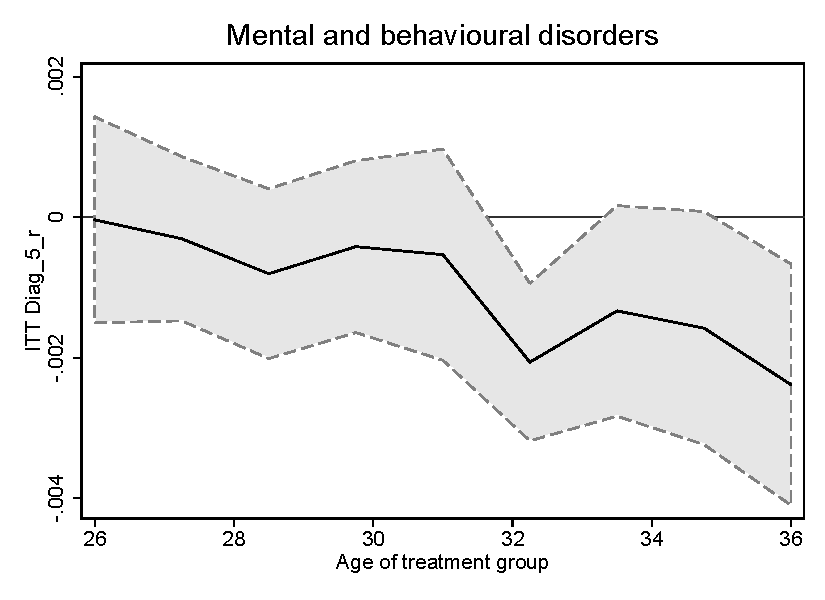
\includegraphics[width=0.99\textwidth]{R1_LC_Diag_5_r}
		\caption{Total}		
	\end{subfigure}
	\begin{subfigure}[t]{0.31\textwidth}
		\centering
		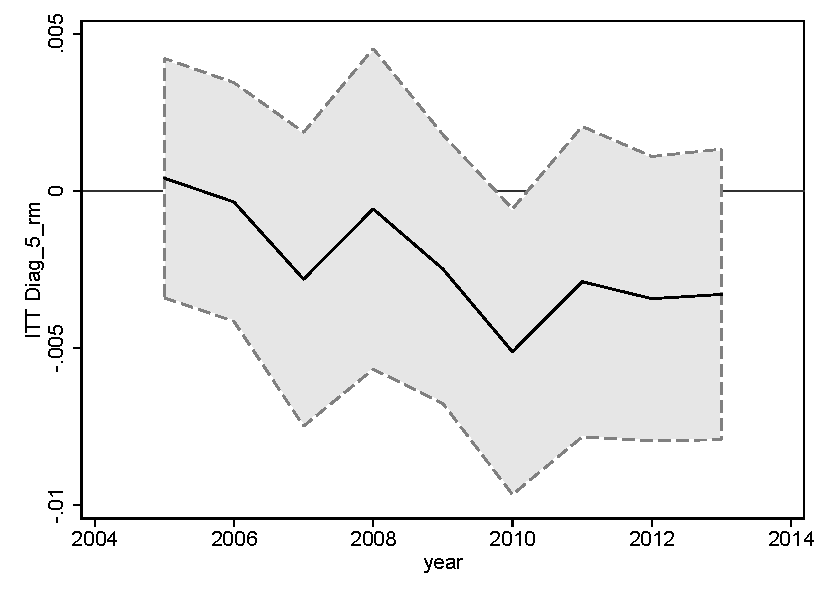
\includegraphics[width=0.99\textwidth]{R1_LC_Diag_5_rm}
		\caption{Men}		
	\end{subfigure}
	\quad
	\begin{subfigure}[t]{0.31\textwidth}
		\centering
		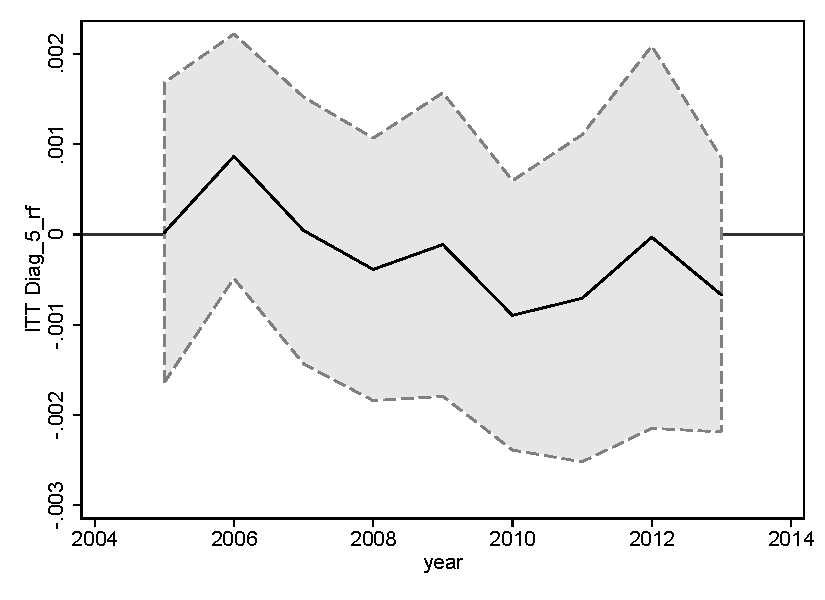
\includegraphics[width=0.99\textwidth]{R1_LC_Diag_5_rf}
		\caption{Women}
	\end{subfigure}
\end{figure}
%%------------------------------------------------------------------------------------
\newpage
\begin{figure}[h]
	\centering
	\begin{subfigure}[t]{0.31\textwidth}
		\centering
		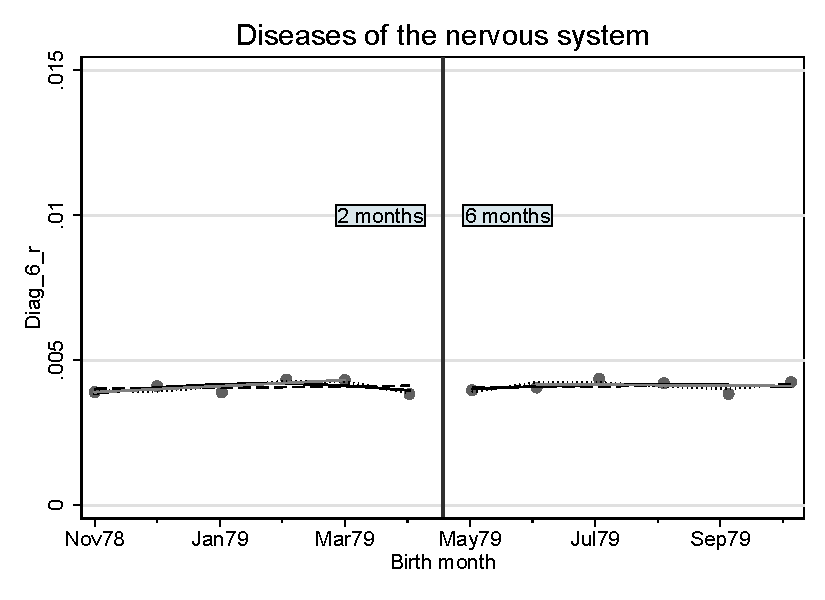
\includegraphics[width=0.99\textwidth]{R1_RD_Diag_6_r_fits}
		\caption{Total}		
	\end{subfigure}
	\begin{subfigure}[t]{0.31\textwidth}
		\centering
		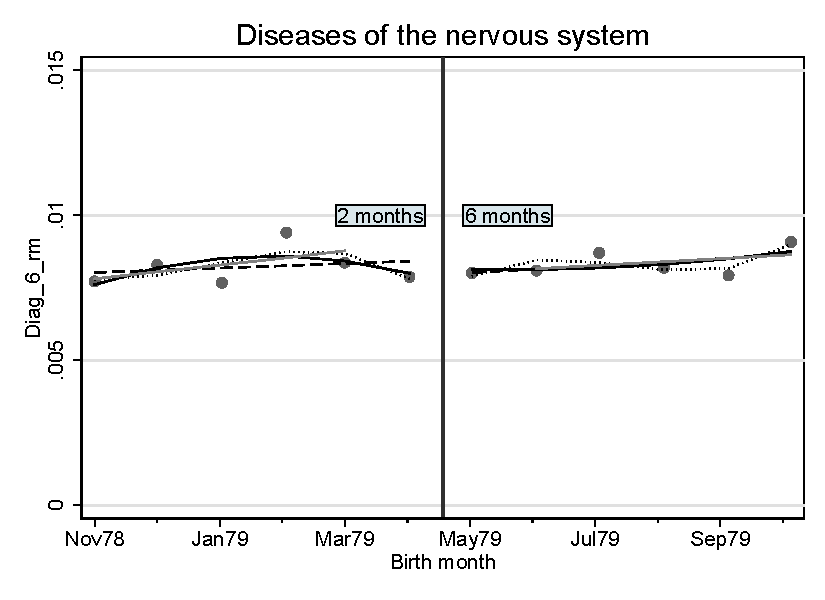
\includegraphics[width=0.99\textwidth]{R1_RD_Diag_6_rm_fits}
		\caption{Men}		
	\end{subfigure}
	\quad
	\begin{subfigure}[t]{0.31\textwidth}
		\centering
		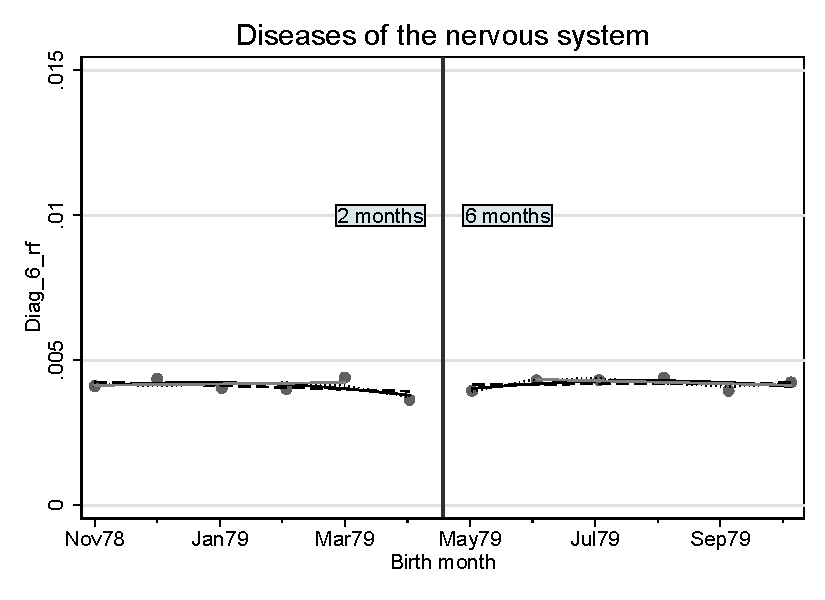
\includegraphics[width=0.99\textwidth]{R1_RD_Diag_6_rf_fits}
		\caption{Women}
	\end{subfigure}
\end{figure}


\begin{table}[h]\centering
\def\sym#1{\ifmmode^{#1}\else\(^{#1}\)\fi}
\begin{tabular}{l*{3}{c}|cccc}
\toprule
&\multicolumn{3}{c}{bandwidth of 6 months} & \multicolumn{4}{c}{different bandwidths} \\
 \cmidrule(lr{1em}){2-4} \cmidrule(lr{1em}){5-8}
 &\multicolumn{1}{c}{(1)}&\multicolumn{1}{c}{(2)}&\multicolumn{1}{c}{(3)}& 1 Month & 2 Months & 4 Months & 6M \& Donut \\
\midrule 
RD Linear           &  -0.0000854         &  -0.0000854         &  -0.0000854         \\
                    &  (0.000268)         &  (0.000279)         &  (0.000279)         \\
RD Quadratic        &    0.000173         &    0.000173         &    0.000173         \\
                    &  (0.000333)         &  (0.000347)         &  (0.000347)         \\
RD Cubic            &    0.000187         &    0.000187         &    0.000187         \\
                    &  (0.000531)         &  (0.000554)         &  (0.000554)         \\
RD Linear Donut     &   -0.000335         &   -0.000335         &   -0.000335         \\
                    &  (0.000225)         &  (0.000236)         &  (0.000236)         \\
\midrule
DDRD: C1-C3 &  0.00000330         &  0.00000330         &  0.00000330         &    0.000257         &  -0.0000950         &  -0.0000441         &  -0.0000474         \\
            &  (0.000129)         &  (0.000130)         &  (0.000130)         &  (0.000227)         &  (0.000211)         &  (0.000161)         &  (0.000133)         \\
DDRD: C2            &   0.0000188         &   0.0000188         &   0.0000188         &    0.000103\sym{***}&   -0.000209         &  -0.0000807         &  0.00000191         \\
                    &  (0.000120)         &  (0.000123)         &  (0.000123)         &  (5.11e-19)         &  (0.000125)         &  (0.000147)         &  (0.000139)         \\
DDRD: C1+C2         &  0.00000383         &  0.00000383         &  0.00000383         &    0.000156         &   -0.000152         &  -0.0000833         &  -0.0000266         \\
                    &  (0.000125)         &  (0.000126)         &  (0.000126)         &  (0.000226)         &  (0.000182)         &  (0.000160)         &  (0.000130)         \\
Birthmonth FE       &           X         &           X         &           X         &                     &                     &                     &                     \\
Time FE             &                     &           X         &           X         &                     &                     &                     &                     \\
Pers covar          &                     &                     &           X         &                     &                     &                     &                     \\
            &\multicolumn{1}{c}{Men}&\multicolumn{1}{c}{Women}\\
\midrule
DDRD: C1-C3 &   0.0000474         &   0.0000608         \\
            &  (0.000326)         &  (0.000150)         \\
DDRD: C2            &-0.000000776         &   0.0000840         \\
                    &  (0.000323)         &  (0.000147)         \\
DDRD: C1+C2         & 0.000000472         &    0.000113         \\
                    &  (0.000333)         &  (0.000162)         \\

\bottomrule
\end{tabular}
\end{table}

\begin{figure}[h!]
	\centering
	\begin{subfigure}[t]{0.31\textwidth}
		\centering
		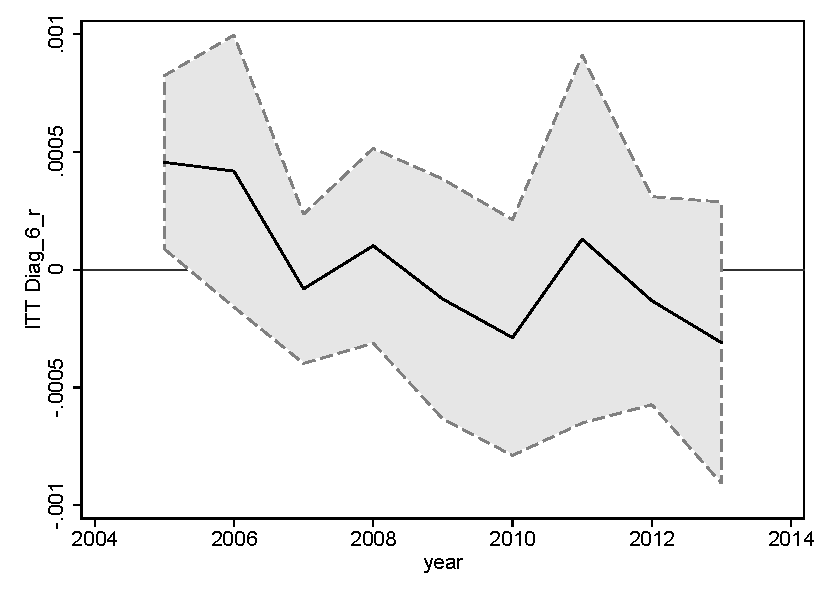
\includegraphics[width=0.99\textwidth]{R1_LC_Diag_6_r}
		\caption{Total}		
	\end{subfigure}
	\begin{subfigure}[t]{0.31\textwidth}
		\centering
		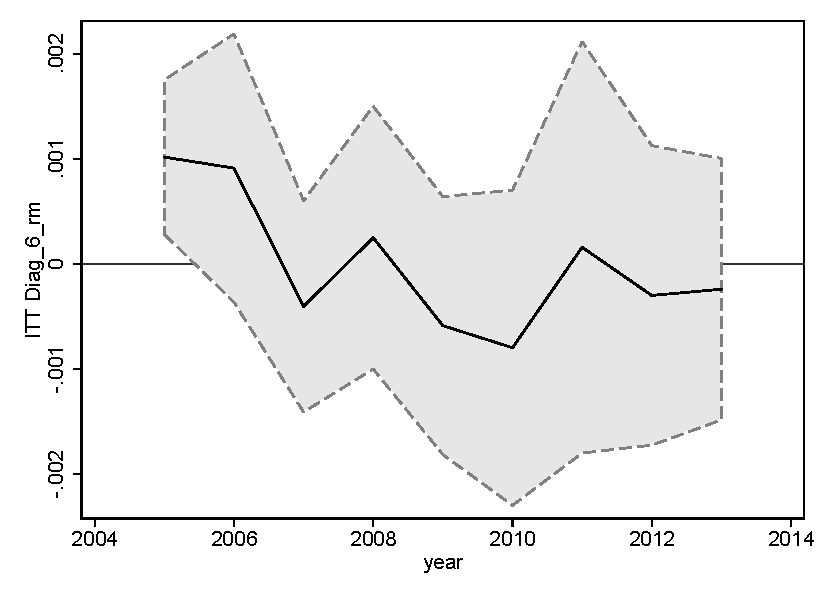
\includegraphics[width=0.99\textwidth]{R1_LC_Diag_6_rm}
		\caption{Men}		
	\end{subfigure}
	\quad
	\begin{subfigure}[t]{0.31\textwidth}
		\centering
		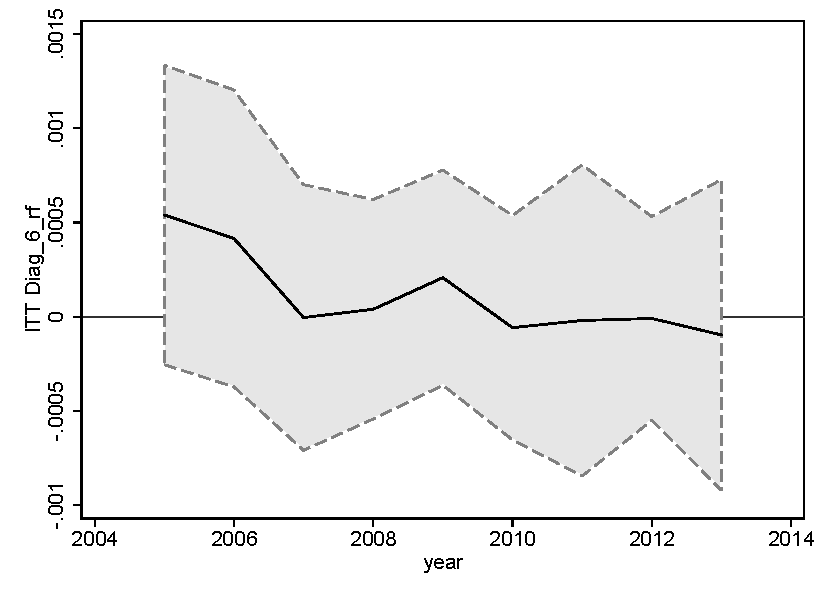
\includegraphics[width=0.99\textwidth]{R1_LC_Diag_6_rf}
		\caption{Women}
	\end{subfigure}
\end{figure}
%%------------------------------------------------------------------------------------
\newpage
\begin{figure}[h]
	\centering
	\begin{subfigure}[t]{0.31\textwidth}
		\centering
		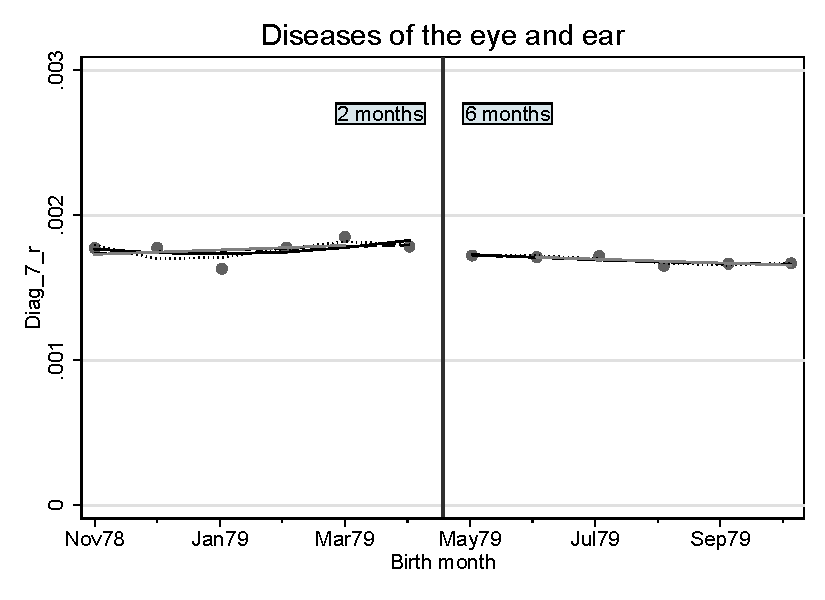
\includegraphics[width=0.99\textwidth]{R1_RD_Diag_7_r_fits}
		\caption{Total}		
	\end{subfigure}
	\begin{subfigure}[t]{0.31\textwidth}
		\centering
		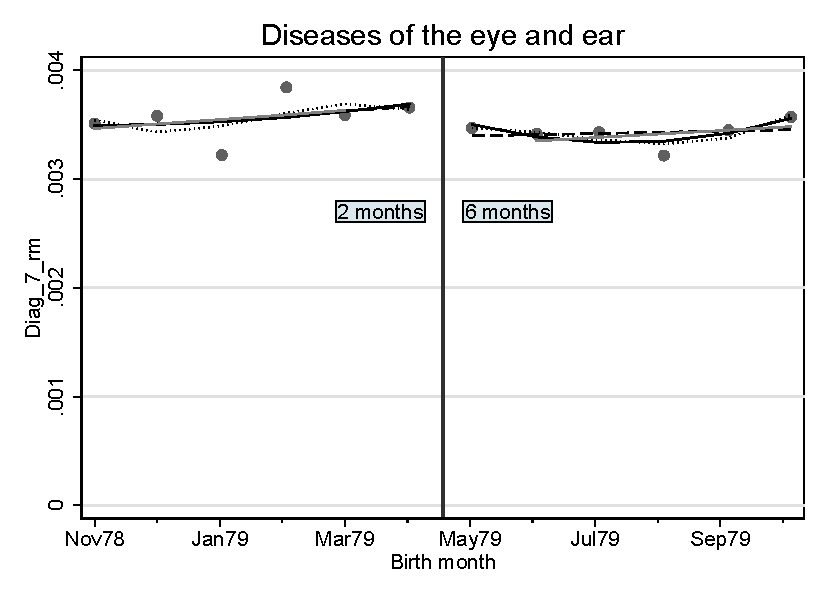
\includegraphics[width=0.99\textwidth]{R1_RD_Diag_7_rm_fits}
		\caption{Men}		
	\end{subfigure}
	\quad
	\begin{subfigure}[t]{0.31\textwidth}
		\centering
		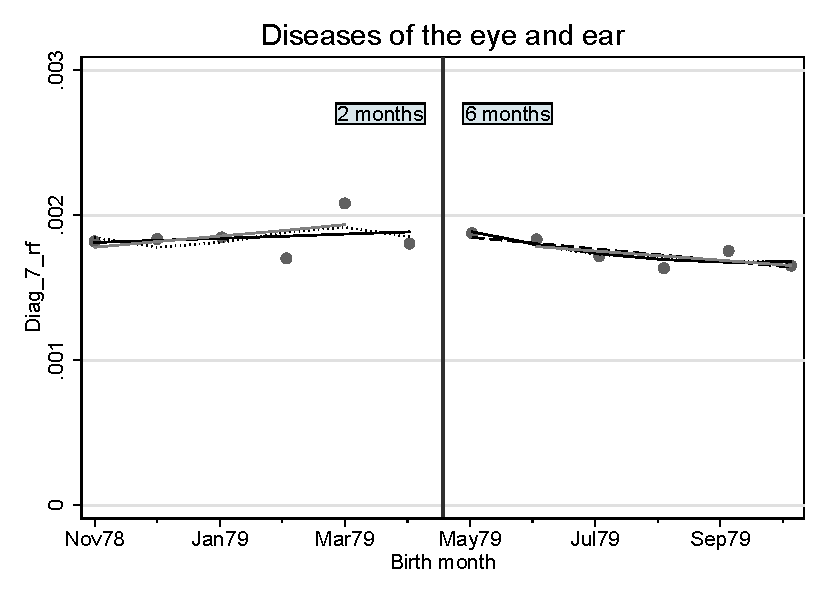
\includegraphics[width=0.99\textwidth]{R1_RD_Diag_7_rf_fits}
		\caption{Women}
	\end{subfigure}
\end{figure}


\begin{table}[h]\centering
\def\sym#1{\ifmmode^{#1}\else\(^{#1}\)\fi}
\begin{tabular}{l*{3}{c}|cccc}
\toprule
&\multicolumn{3}{c}{bandwidth of 6 months} & \multicolumn{4}{c}{different bandwidths} \\
 \cmidrule(lr{1em}){2-4} \cmidrule(lr{1em}){5-8}
 &\multicolumn{1}{c}{(1)}&\multicolumn{1}{c}{(2)}&\multicolumn{1}{c}{(3)}& 1 Month & 2 Months & 4 Months & 6M \& Donut \\
\midrule 
RD Linear           &  -0.0000703\sym{*}  &  -0.0000703         &  -0.0000703         \\
                    & (0.0000390)         & (0.0000406)         & (0.0000406)         \\
RD Quadratic        &   -0.000142         &   -0.000142         &   -0.000142         \\
                    &  (0.000103)         &  (0.000107)         &  (0.000107)         \\
RD Cubic            &   0.0000303         &   0.0000303         &   0.0000303         \\
                    &  (0.000134)         &  (0.000140)         &  (0.000140)         \\
RD Linear Donut     &  -0.0000849         &  -0.0000849         &  -0.0000849         \\
                    & (0.0000759)         & (0.0000797)         & (0.0000797)         \\
\midrule
DDRD: C1-C3 &  -0.0000664         &  -0.0000664         &  -0.0000664         &  -0.0000311         &  -0.0000773         &  -0.0000610         &  -0.0000735         \\
            & (0.0000446)         & (0.0000451)         & (0.0000451)         &  (0.000142)         & (0.0000815)         & (0.0000507)         & (0.0000449)         \\
DDRD: C2            &   -0.000170\sym{***}&   -0.000170\sym{***}&   -0.000170\sym{***}&   -0.000367\sym{***}&   -0.000297\sym{***}&   -0.000213\sym{***}&   -0.000131\sym{***}\\
                    & (0.0000392)         & (0.0000400)         & (0.0000400)         &  (2.73e-19)         & (0.0000340)         & (0.0000454)         & (0.0000335)         \\
DDRD: C1+C2         &  -0.0000639         &  -0.0000639         &  -0.0000639         &   -0.000115         &   -0.000113         &  -0.0000790         &  -0.0000536         \\
                    & (0.0000413)         & (0.0000418)         & (0.0000418)         &  (0.000165)         & (0.0000846)         & (0.0000497)         & (0.0000374)         \\
Birthmonth FE       &           X         &           X         &           X         &                     &                     &                     &                     \\
Time FE             &                     &           X         &           X         &                     &                     &                     &                     \\
Pers covar          &                     &                     &           X         &                     &                     &                     &                     \\
            &\multicolumn{1}{c}{Men}&\multicolumn{1}{c}{Women}\\
\midrule
DDRD: C1-C3 &   -0.000110         &  -0.0000959         \\
            &  (0.000122)         & (0.0000680)         \\
DDRD: C2            &   -0.000125         &   -0.000104\sym{*}  \\
                    &  (0.000120)         & (0.0000601)         \\
DDRD: C1+C2         &   -0.000352\sym{**} &   -0.000193\sym{***}\\
                    &  (0.000137)         & (0.0000604)         \\

\bottomrule
\end{tabular}
\end{table}

\begin{figure}[h!]
	\centering
	\begin{subfigure}[t]{0.31\textwidth}
		\centering
		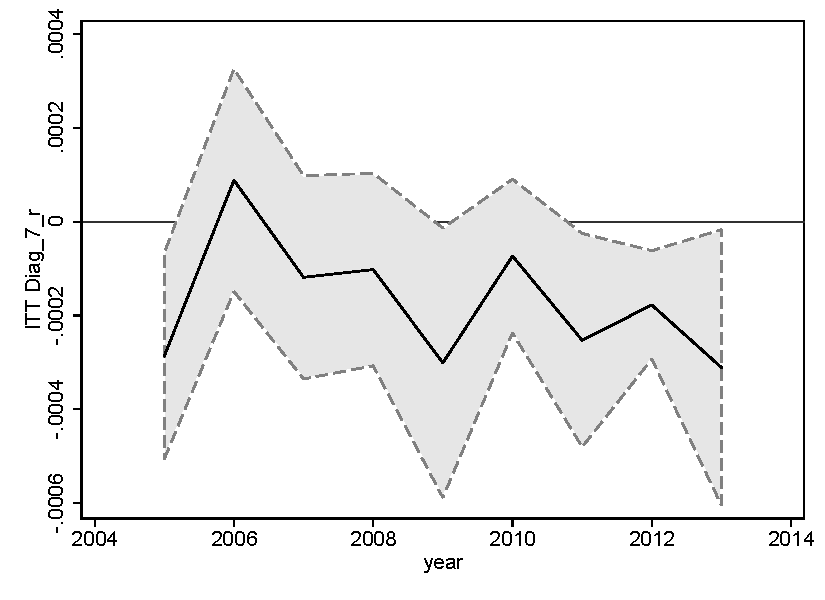
\includegraphics[width=0.99\textwidth]{R1_LC_Diag_7_r}
		\caption{Total}		
	\end{subfigure}
	\begin{subfigure}[t]{0.31\textwidth}
		\centering
		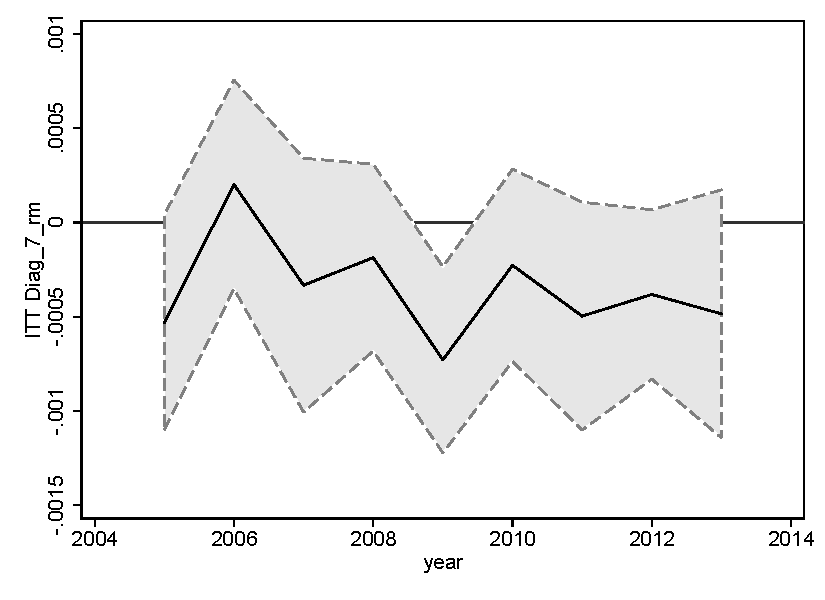
\includegraphics[width=0.99\textwidth]{R1_LC_Diag_7_rm}
		\caption{Men}		
	\end{subfigure}
	\quad
	\begin{subfigure}[t]{0.31\textwidth}
		\centering
		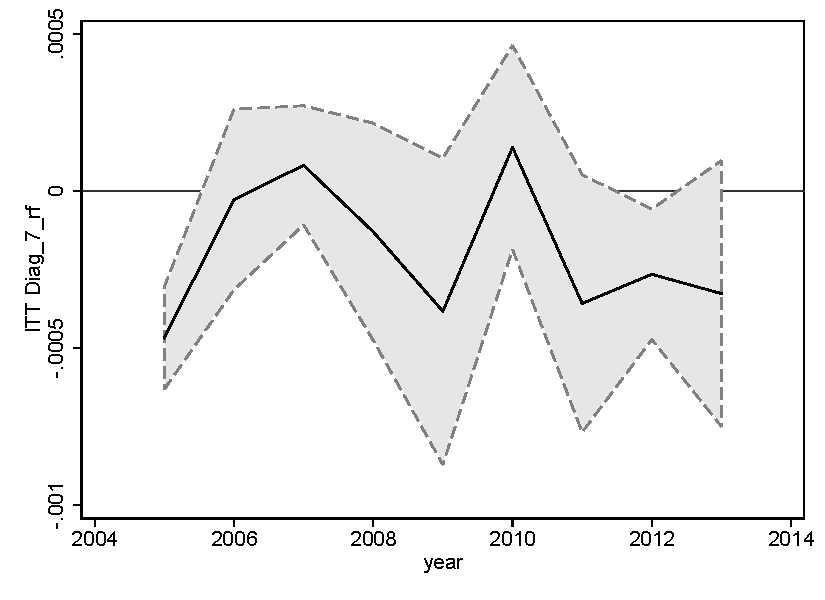
\includegraphics[width=0.99\textwidth]{R1_LC_Diag_7_rf}
		\caption{Women}
	\end{subfigure}
\end{figure}
%%------------------------------------------------------------------------------------
\newpage
\begin{figure}[h]
	\centering
	\begin{subfigure}[t]{0.31\textwidth}
		\centering
		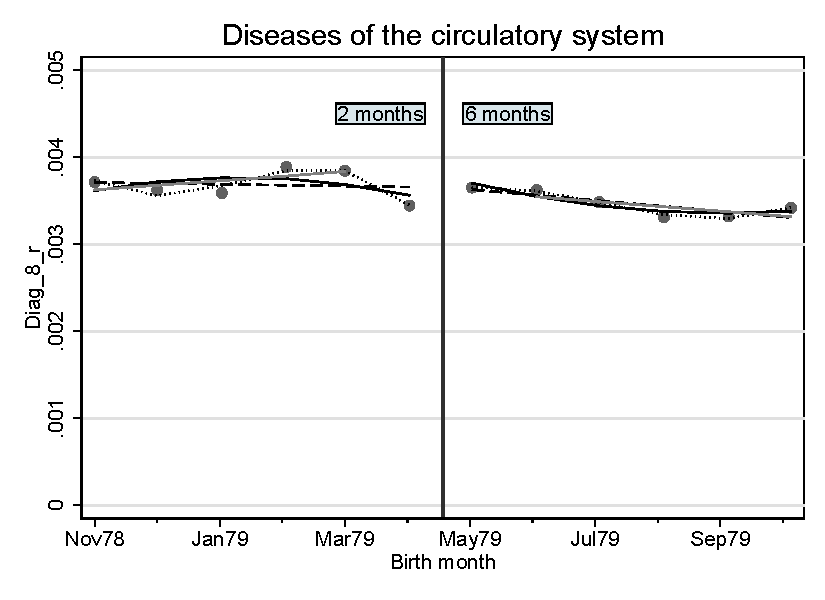
\includegraphics[width=0.99\textwidth]{R1_RD_Diag_8_r_fits}
		\caption{Total}		
	\end{subfigure}
	\begin{subfigure}[t]{0.31\textwidth}
		\centering
		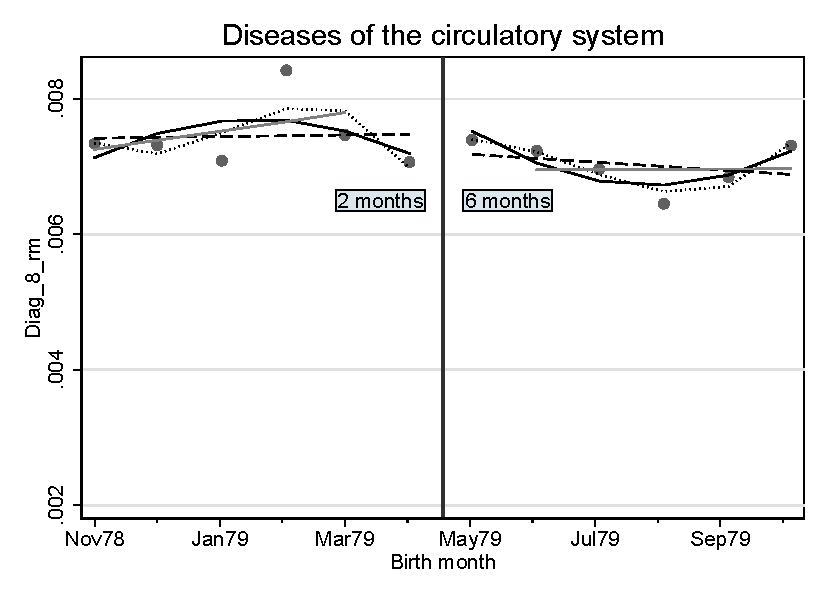
\includegraphics[width=0.99\textwidth]{R1_RD_Diag_8_rm_fits}
		\caption{Men}		
	\end{subfigure}
	\quad
	\begin{subfigure}[t]{0.31\textwidth}
		\centering
		\includegraphics[width=0.99\textwidth]{R1_RD_Diag_8_rf_fits}
		\caption{Women}
	\end{subfigure}
\end{figure}


\begin{table}[h]\centering
\def\sym#1{\ifmmode^{#1}\else\(^{#1}\)\fi}
\begin{tabular}{l*{3}{c}|cccc}
\toprule
&\multicolumn{3}{c}{bandwidth of 6 months} & \multicolumn{4}{c}{different bandwidths} \\
 \cmidrule(lr{1em}){2-4} \cmidrule(lr{1em}){5-8}
 &\multicolumn{1}{c}{(1)}&\multicolumn{1}{c}{(2)}&\multicolumn{1}{c}{(3)}& 1 Month & 2 Months & 4 Months & 6M \& Donut \\
\midrule 
RD Linear           &   0.0000456         &   0.0000456         &   0.0000456         \\
                    &  (0.000191)         &  (0.000199)         &  (0.000199)         \\
RD Quadratic        &    0.000513\sym{*}  &    0.000513\sym{*}  &    0.000513\sym{*}  \\
                    &  (0.000260)         &  (0.000271)         &  (0.000271)         \\
RD Cubic            &     0.00109\sym{***}&     0.00109\sym{***}&     0.00109\sym{***}\\
                    &  (0.000124)         &  (0.000129)         &  (0.000129)         \\
RD Linear Donut     &   -0.000283\sym{*}  &   -0.000283\sym{*}  &   -0.000283\sym{*}  \\
                    &  (0.000144)         &  (0.000151)         &  (0.000151)         \\
\midrule
DDRD: C1-C3 &   -0.000101         &   -0.000101         &   -0.000101         &    0.000271         &   0.0000321         &   -0.000125         &   -0.000176         \\
            &  (0.000147)         &  (0.000149)         &  (0.000149)         &  (0.000481)         &  (0.000287)         &  (0.000178)         &  (0.000146)         \\
DDRD: C2            &   -0.000140\sym{**} &   -0.000140\sym{**} &   -0.000140\sym{**} &  -0.0000794\sym{***}&   -0.000142\sym{**} &   -0.000178\sym{***}&   -0.000153\sym{**} \\
                    & (0.0000593)         & (0.0000605)         & (0.0000605)         &  (1.02e-18)         & (0.0000599)         & (0.0000462)         & (0.0000678)         \\
DDRD: C1+C2         &   -0.000120         &   -0.000120         &   -0.000120         &    0.000208         & -0.00000522         &   -0.000159         &   -0.000186\sym{*}  \\
                    &  (0.000101)         &  (0.000102)         &  (0.000102)         &  (0.000263)         &  (0.000181)         &  (0.000115)         &  (0.000101)         \\
Birthmonth FE       &           X         &           X         &           X         &                     &                     &                     &                     \\
Time FE             &                     &           X         &           X         &                     &                     &                     &                     \\
Pers covar          &                     &                     &           X         &                     &                     &                     &                     \\
            &\multicolumn{1}{c}{Men}&\multicolumn{1}{c}{Women}\\
\midrule
DDRD: C1-C3 &   -0.000166         &   0.0000132         \\
            &  (0.000356)         &  (0.000148)         \\
DDRD: C2            &   -0.000247         &  -0.0000103         \\
                    &  (0.000288)         &  (0.000114)         \\
DDRD: C1+C2         &   -0.000307         &  -0.0000222         \\
                    &  (0.000268)         & (0.0000826)         \\

\bottomrule
\end{tabular}
\end{table}

\begin{figure}[h!]
	\centering
	\begin{subfigure}[t]{0.31\textwidth}
		\centering
		\includegraphics[width=0.99\textwidth]{R1_LC_Diag_8_r}
		\caption{Total}		
	\end{subfigure}
	\begin{subfigure}[t]{0.31\textwidth}
		\centering
		\includegraphics[width=0.99\textwidth]{R1_LC_Diag_8_rm}
		\caption{Men}		
	\end{subfigure}
	\quad
	\begin{subfigure}[t]{0.31\textwidth}
		\centering
		\includegraphics[width=0.99\textwidth]{R1_LC_Diag_8_rf}
		\caption{Women}
	\end{subfigure}
\end{figure}
%%------------------------------------------------------------------------------------
\newpage
\begin{figure}[h]
	\centering
	\begin{subfigure}[t]{0.31\textwidth}
		\centering
		\includegraphics[width=0.99\textwidth]{R1_RD_Diag_9_r_fits}
		\caption{Total}		
	\end{subfigure}
	\begin{subfigure}[t]{0.31\textwidth}
		\centering
		\includegraphics[width=0.99\textwidth]{R1_RD_Diag_9_rm_fits}
		\caption{Men}		
	\end{subfigure}
	\quad
	\begin{subfigure}[t]{0.31\textwidth}
		\centering
		\includegraphics[width=0.99\textwidth]{R1_RD_Diag_9_rf_fits}
		\caption{Women}
	\end{subfigure}
\end{figure}


\begin{table}[h]\centering
\def\sym#1{\ifmmode^{#1}\else\(^{#1}\)\fi}
\begin{tabular}{l*{3}{c}|cccc}
\toprule
&\multicolumn{3}{c}{bandwidth of 6 months} & \multicolumn{4}{c}{different bandwidths} \\
 \cmidrule(lr{1em}){2-4} \cmidrule(lr{1em}){5-8}
 &\multicolumn{1}{c}{(1)}&\multicolumn{1}{c}{(2)}&\multicolumn{1}{c}{(3)}& 1 Month & 2 Months & 4 Months & 6M \& Donut \\
\midrule 
RD Linear           &   -0.000415         &   -0.000415         &   -0.000415         \\
                    &  (0.000311)         &  (0.000323)         &  (0.000323)         \\
RD Quadratic        &    0.000140         &    0.000140         &    0.000140         \\
                    &  (0.000512)         &  (0.000533)         &  (0.000533)         \\
RD Cubic            &   -0.000269         &   -0.000269         &   -0.000269         \\
                    &  (0.000781)         &  (0.000815)         &  (0.000815)         \\
RD Linear Donut     &   -0.000733\sym{*}  &   -0.000733\sym{*}  &   -0.000733\sym{*}  \\
                    &  (0.000357)         &  (0.000375)         &  (0.000375)         \\
\midrule
DDRD: C1-C3 &   -0.000129         &   -0.000129         &   -0.000129         &    0.000138         &   -0.000229         &   -0.000142         &   -0.000183         \\
            &  (0.000139)         &  (0.000140)         &  (0.000140)         &  (0.000118)         &  (0.000174)         &  (0.000137)         &  (0.000159)         \\
DDRD: C2            &  -0.0000948         &  -0.0000948         &  -0.0000948         &  -0.0000218\sym{***}&   -0.000287\sym{**} &   -0.000171\sym{*}  &   -0.000109         \\
                    &  (0.000138)         &  (0.000141)         &  (0.000141)         &  (4.35e-19)         &  (0.000106)         & (0.0000933)         &  (0.000166)         \\
DDRD: C1+C2         &   -0.000158         &   -0.000158         &   -0.000158         &    0.000154         &   -0.000200         &   -0.000174         &   -0.000220         \\
                    &  (0.000148)         &  (0.000150)         &  (0.000150)         &  (0.000156)         &  (0.000182)         &  (0.000152)         &  (0.000168)         \\
Birthmonth FE       &           X         &           X         &           X         &                     &                     &                     &                     \\
Time FE             &                     &           X         &           X         &                     &                     &                     &                     \\
Pers covar          &                     &                     &           X         &                     &                     &                     &                     \\
            &\multicolumn{1}{c}{Men}&\multicolumn{1}{c}{Women}\\
\midrule
DDRD: C1-C3 &   -0.000171         &  -0.0000774         \\
            &  (0.000462)         &  (0.000206)         \\
DDRD: C2            &   -0.000316         &  -0.0000896         \\
                    &  (0.000475)         &  (0.000206)         \\
DDRD: C1+C2         &   -0.000252         &   0.0000896         \\
                    &  (0.000510)         &  (0.000218)         \\

\bottomrule
\end{tabular}
\end{table}

\begin{figure}[h!]
	\centering
	\begin{subfigure}[t]{0.31\textwidth}
		\centering
		\includegraphics[width=0.99\textwidth]{R1_LC_Diag_9_r}
		\caption{Total}		
	\end{subfigure}
	\begin{subfigure}[t]{0.31\textwidth}
		\centering
		\includegraphics[width=0.99\textwidth]{R1_LC_Diag_9_rm}
		\caption{Men}		
	\end{subfigure}
	\quad
	\begin{subfigure}[t]{0.31\textwidth}
		\centering
		\includegraphics[width=0.99\textwidth]{R1_LC_Diag_9_rf}
		\caption{Women}
	\end{subfigure}
\end{figure}
%%------------------------------------------------------------------------------------
\newpage
\begin{figure}[h]
	\centering
	\begin{subfigure}[t]{0.31\textwidth}
		\centering
		\includegraphics[width=0.99\textwidth]{R1_RD_Diag_10_r_fits}
		\caption{Total}		
	\end{subfigure}
	\begin{subfigure}[t]{0.31\textwidth}
		\centering
		\includegraphics[width=0.99\textwidth]{R1_RD_Diag_10_rm_fits}
		\caption{Men}		
	\end{subfigure}
	\quad
	\begin{subfigure}[t]{0.31\textwidth}
		\centering
		\includegraphics[width=0.99\textwidth]{R1_RD_Diag_10_rf_fits}
		\caption{Women}
	\end{subfigure}
\end{figure}


\begin{table}[h]\centering
\def\sym#1{\ifmmode^{#1}\else\(^{#1}\)\fi}
\begin{tabular}{l*{3}{c}|cccc}
\toprule
&\multicolumn{3}{c}{bandwidth of 6 months} & \multicolumn{4}{c}{different bandwidths} \\
 \cmidrule(lr{1em}){2-4} \cmidrule(lr{1em}){5-8}
 &\multicolumn{1}{c}{(1)}&\multicolumn{1}{c}{(2)}&\multicolumn{1}{c}{(3)}& 1 Month & 2 Months & 4 Months & 6M \& Donut \\
\midrule 
RD Linear           &   -0.000261         &   -0.000261         &   -0.000261         \\
                    &  (0.000407)         &  (0.000424)         &  (0.000424)         \\
RD Quadratic        &    0.000617         &    0.000617         &    0.000617         \\
                    &  (0.000776)         &  (0.000808)         &  (0.000808)         \\
RD Cubic            &     0.00125         &     0.00125         &     0.00125         \\
                    &   (0.00149)         &   (0.00155)         &   (0.00155)         \\
RD Linear Donut     &   -0.000815         &   -0.000815         &   -0.000815         \\
                    &  (0.000719)         &  (0.000755)         &  (0.000755)         \\
\midrule
DDRD: C1-C3 &  -0.0000914         &  -0.0000914         &  -0.0000914         &    0.000618         &    0.000191         &   -0.000134         &   -0.000233         \\
            &  (0.000198)         &  (0.000200)         &  (0.000200)         &  (0.000419)         &  (0.000287)         &  (0.000247)         &  (0.000208)         \\
DDRD: C2            &   -0.000307         &   -0.000307         &   -0.000307         &  -0.0000497\sym{***}&   -0.000274         &   -0.000485\sym{*}  &   -0.000358         \\
                    &  (0.000195)         &  (0.000199)         &  (0.000199)         &  (1.65e-18)         &  (0.000152)         &  (0.000229)         &  (0.000233)         \\
DDRD: C1+C2         &   -0.000200         &   -0.000200         &   -0.000200         &    0.000371         &   0.0000125         &   -0.000330         &   -0.000314         \\
                    &  (0.000198)         &  (0.000200)         &  (0.000200)         &  (0.000354)         &  (0.000241)         &  (0.000250)         &  (0.000217)         \\
Birthmonth FE       &           X         &           X         &           X         &                     &                     &                     &                     \\
Time FE             &                     &           X         &           X         &                     &                     &                     &                     \\
Pers covar          &                     &                     &           X         &                     &                     &                     &                     \\
            &\multicolumn{1}{c}{Men}&\multicolumn{1}{c}{Women}\\
\midrule
DDRD: C1-C3 &  -0.0000521         &   -0.000350         \\
            &  (0.000811)         &  (0.000271)         \\
DDRD: C2            &   -0.000415         &   -0.000353         \\
                    &  (0.000814)         &  (0.000251)         \\
DDRD: C1+C2         &   -0.000712         &   -0.000500\sym{*}  \\
                    &  (0.000912)         &  (0.000249)         \\

\bottomrule
\end{tabular}
\end{table}

\begin{figure}[h!]
	\centering
	\begin{subfigure}[t]{0.31\textwidth}
		\centering
		\includegraphics[width=0.99\textwidth]{R1_LC_Diag_10_r}
		\caption{Total}		
	\end{subfigure}
	\begin{subfigure}[t]{0.31\textwidth}
		\centering
		\includegraphics[width=0.99\textwidth]{R1_LC_Diag_10_rm}
		\caption{Men}		
	\end{subfigure}
	\quad
	\begin{subfigure}[t]{0.31\textwidth}
		\centering
		\includegraphics[width=0.99\textwidth]{R1_LC_Diag_10_rf}
		\caption{Women}
	\end{subfigure}
\end{figure}
%%------------------------------------------------------------------------------------
\newpage
\begin{figure}[h]
	\centering
	\begin{subfigure}[t]{0.31\textwidth}
		\centering
		\includegraphics[width=0.99\textwidth]{R1_RD_Diag_11_r_fits}
		\caption{Total}		
	\end{subfigure}
	\begin{subfigure}[t]{0.31\textwidth}
		\centering
		\includegraphics[width=0.99\textwidth]{R1_RD_Diag_11_rm_fits}
		\caption{Men}		
	\end{subfigure}
	\quad
	\begin{subfigure}[t]{0.31\textwidth}
		\centering
		\includegraphics[width=0.99\textwidth]{R1_RD_Diag_11_rf_fits}
		\caption{Women}
	\end{subfigure}
\end{figure}


\begin{table}[h]\centering
\def\sym#1{\ifmmode^{#1}\else\(^{#1}\)\fi}
\begin{tabular}{l*{3}{c}|cccc}
\toprule
&\multicolumn{3}{c}{bandwidth of 6 months} & \multicolumn{4}{c}{different bandwidths} \\
 \cmidrule(lr{1em}){2-4} \cmidrule(lr{1em}){5-8}
 &\multicolumn{1}{c}{(1)}&\multicolumn{1}{c}{(2)}&\multicolumn{1}{c}{(3)}& 1 Month & 2 Months & 4 Months & 6M \& Donut \\
\midrule 
RD Linear           &    0.000109         &    0.000109         &    0.000109         \\
                    &  (0.000133)         &  (0.000138)         &  (0.000138)         \\
RD Quadratic        &    0.000277         &    0.000277         &    0.000277         \\
                    &  (0.000256)         &  (0.000266)         &  (0.000266)         \\
RD Cubic            &   -0.000728\sym{*}  &   -0.000728\sym{*}  &   -0.000728\sym{*}  \\
                    &  (0.000380)         &  (0.000396)         &  (0.000396)         \\
RD Linear Donut     &    0.000196         &    0.000196         &    0.000196         \\
                    &  (0.000241)         &  (0.000253)         &  (0.000253)         \\
\midrule
DDRD: C1-C3 &    0.000105         &    0.000105         &    0.000105         &    0.000212\sym{*}  &    0.000244\sym{***}&    0.000136\sym{**} &   0.0000832         \\
            & (0.0000653)         & (0.0000659)         & (0.0000659)         & (0.0000960)         & (0.0000826)         & (0.0000657)         & (0.0000751)         \\
DDRD: C2            &   0.0000888         &   0.0000888         &   0.0000888         &   0.0000315\sym{***}&    0.000247\sym{**} &    0.000114         &    0.000100         \\
                    & (0.0000573)         & (0.0000585)         & (0.0000585)         &  (2.73e-19)         & (0.0000980)         & (0.0000716)         & (0.0000669)         \\
DDRD: C1+C2         &    0.000112         &    0.000112         &    0.000112         &    0.000240         &    0.000290\sym{**} &    0.000137\sym{*}  &   0.0000866         \\
                    & (0.0000673)         & (0.0000682)         & (0.0000682)         &  (0.000130)         & (0.0000984)         & (0.0000748)         & (0.0000760)         \\
Birthmonth FE       &           X         &           X         &           X         &                     &                     &                     &                     \\
Time FE             &                     &           X         &           X         &                     &                     &                     &                     \\
Pers covar          &                     &                     &           X         &                     &                     &                     &                     \\
            &\multicolumn{1}{c}{Men}&\multicolumn{1}{c}{Women}\\
\midrule
DDRD: C1-C3 &    0.000243         &   0.0000834         \\
            &  (0.000206)         & (0.0000838)         \\
DDRD: C2            &    0.000225         &    0.000125         \\
                    &  (0.000215)         & (0.0000775)         \\
DDRD: C1+C2         &    0.000158         &   0.0000601         \\
                    &  (0.000237)         & (0.0000507)         \\

\bottomrule
\end{tabular}
\end{table}

\begin{figure}[h!]
	\centering
	\begin{subfigure}[t]{0.31\textwidth}
		\centering
		\includegraphics[width=0.99\textwidth]{R1_LC_Diag_11_r}
		\caption{Total}		
	\end{subfigure}
	\begin{subfigure}[t]{0.31\textwidth}
		\centering
		\includegraphics[width=0.99\textwidth]{R1_LC_Diag_11_rm}
		\caption{Men}		
	\end{subfigure}
	\quad
	\begin{subfigure}[t]{0.31\textwidth}
		\centering
		\includegraphics[width=0.99\textwidth]{R1_LC_Diag_11_rf}
		\caption{Women}
	\end{subfigure}
\end{figure}
%%------------------------------------------------------------------------------------
\newpage
\begin{figure}[h]
	\centering
	\begin{subfigure}[t]{0.31\textwidth}
		\centering
		\includegraphics[width=0.99\textwidth]{R1_RD_Diag_12_r_fits}
		\caption{Total}		
	\end{subfigure}
	\begin{subfigure}[t]{0.31\textwidth}
		\centering
		\includegraphics[width=0.99\textwidth]{R1_RD_Diag_12_rm_fits}
		\caption{Men}		
	\end{subfigure}
	\quad
	\begin{subfigure}[t]{0.31\textwidth}
		\centering
		\includegraphics[width=0.99\textwidth]{R1_RD_Diag_12_rf_fits}
		\caption{Women}
	\end{subfigure}
\end{figure}


\begin{table}[h]\centering
\def\sym#1{\ifmmode^{#1}\else\(^{#1}\)\fi}
\begin{tabular}{l*{3}{c}|cccc}
\toprule
&\multicolumn{3}{c}{bandwidth of 6 months} & \multicolumn{4}{c}{different bandwidths} \\
 \cmidrule(lr{1em}){2-4} \cmidrule(lr{1em}){5-8}
 &\multicolumn{1}{c}{(1)}&\multicolumn{1}{c}{(2)}&\multicolumn{1}{c}{(3)}& 1 Month & 2 Months & 4 Months & 6M \& Donut \\
\midrule 
RD Linear           &   0.0000626         &   0.0000626         &   0.0000626         \\
                    &  (0.000225)         &  (0.000234)         &  (0.000234)         \\
RD Quadratic        &    0.000791\sym{*}  &    0.000791\sym{*}  &    0.000791\sym{*}  \\
                    &  (0.000418)         &  (0.000435)         &  (0.000435)         \\
RD Cubic            &   -0.000555         &   -0.000555         &   -0.000555         \\
                    &  (0.000723)         &  (0.000753)         &  (0.000753)         \\
RD Linear Donut     &   -0.000151         &   -0.000151         &   -0.000151         \\
                    &  (0.000390)         &  (0.000409)         &  (0.000409)         \\
\midrule
DDRD: C1-C3 &  0.00000944         &  0.00000944         &  0.00000944         &    0.000213         &    0.000199         &  -0.0000188         &  -0.0000312         \\
            &  (0.000243)         &  (0.000245)         &  (0.000245)         &  (0.000685)         &  (0.000391)         &  (0.000270)         &  (0.000258)         \\
DDRD: C2            &   0.0000469         &   0.0000469         &   0.0000469         &   -0.000284\sym{***}&   0.0000239         &   0.0000165         &    0.000113         \\
                    &  (0.000147)         &  (0.000150)         &  (0.000150)         &  (1.62e-18)         &  (0.000121)         &  (0.000141)         &  (0.000168)         \\
DDRD: C1+C2         &   0.0000381         &   0.0000381         &   0.0000381         &   0.0000450         &    0.000160         &  -0.0000302         &   0.0000368         \\
                    &  (0.000181)         &  (0.000184)         &  (0.000184)         &  (0.000443)         &  (0.000243)         &  (0.000204)         &  (0.000193)         \\
Birthmonth FE       &           X         &           X         &           X         &                     &                     &                     &                     \\
Time FE             &                     &           X         &           X         &                     &                     &                     &                     \\
Pers covar          &                     &                     &           X         &                     &                     &                     &                     \\
            &\multicolumn{1}{c}{Men}&\multicolumn{1}{c}{Women}\\
\midrule
DDRD: C1-C3 &   0.0000912         &    0.000148         \\
            &  (0.000642)         &  (0.000265)         \\
DDRD: C2            &   0.0000633         &    0.000293         \\
                    &  (0.000535)         &  (0.000217)         \\
DDRD: C1+C2         &   0.0000305         &    0.000334         \\
                    &  (0.000525)         &  (0.000242)         \\

\bottomrule
\end{tabular}
\end{table}

\begin{figure}[h!]
	\centering
	\begin{subfigure}[t]{0.31\textwidth}
		\centering
		\includegraphics[width=0.99\textwidth]{R1_LC_Diag_12_r}
		\caption{Total}		
	\end{subfigure}
	\begin{subfigure}[t]{0.31\textwidth}
		\centering
		\includegraphics[width=0.99\textwidth]{R1_LC_Diag_12_rm}
		\caption{Men}		
	\end{subfigure}
	\quad
	\begin{subfigure}[t]{0.31\textwidth}
		\centering
		\includegraphics[width=0.99\textwidth]{R1_LC_Diag_12_rf}
		\caption{Women}
	\end{subfigure}
\end{figure}
%%------------------------------------------------------------------------------------
\newpage
\begin{figure}[h]
	\centering
	\begin{subfigure}[t]{0.31\textwidth}
		\centering
		\includegraphics[width=0.99\textwidth]{R1_RD_Diag_13_r_fits}
		\caption{Total}		
	\end{subfigure}
	\begin{subfigure}[t]{0.31\textwidth}
		\centering
		\includegraphics[width=0.99\textwidth]{R1_RD_Diag_13_rm_fits}
		\caption{Men}		
	\end{subfigure}
	\quad
	\begin{subfigure}[t]{0.31\textwidth}
		\centering
		\includegraphics[width=0.99\textwidth]{R1_RD_Diag_13_rf_fits}
		\caption{Women}
	\end{subfigure}
\end{figure}


\begin{table}[h]\centering
\def\sym#1{\ifmmode^{#1}\else\(^{#1}\)\fi}
\begin{tabular}{l*{3}{c}|cccc}
\toprule
&\multicolumn{3}{c}{bandwidth of 6 months} & \multicolumn{4}{c}{different bandwidths} \\
 \cmidrule(lr{1em}){2-4} \cmidrule(lr{1em}){5-8}
 &\multicolumn{1}{c}{(1)}&\multicolumn{1}{c}{(2)}&\multicolumn{1}{c}{(3)}& 1 Month & 2 Months & 4 Months & 6M \& Donut \\
\midrule 
RD Linear           &  -0.0000801         &  -0.0000801         &  -0.0000801         \\
                    &  (0.000339)         &  (0.000353)         &  (0.000353)         \\
RD Quadratic        &    0.000433         &    0.000433         &    0.000433         \\
                    &  (0.000583)         &  (0.000607)         &  (0.000607)         \\
RD Cubic            &    0.000719         &    0.000719         &    0.000719         \\
                    &  (0.000929)         &  (0.000969)         &  (0.000969)         \\
RD Linear Donut     &   -0.000439         &   -0.000439         &   -0.000439         \\
                    &  (0.000435)         &  (0.000457)         &  (0.000457)         \\
\midrule
DDRD: C1-C3 &  -0.0000441         &  -0.0000441         &  -0.0000441         &    0.000388         &  0.00000438         &  -0.0000196         &   -0.000131         \\
            &  (0.000171)         &  (0.000173)         &  (0.000173)         &  (0.000391)         &  (0.000280)         &  (0.000208)         &  (0.000169)         \\
DDRD: C2            &   -0.000115         &   -0.000115         &   -0.000115         &   0.0000159\sym{***}&   -0.000156         &  -0.0000721         &   -0.000141         \\
                    &  (0.000166)         &  (0.000170)         &  (0.000170)         &  (1.76e-18)         &  (0.000151)         &  (0.000195)         &  (0.000177)         \\
DDRD: C1+C2         &  -0.0000195         &  -0.0000195         &  -0.0000195         &    0.000294         &  -0.0000841         &  -0.0000612         &  -0.0000821         \\
                    &  (0.000172)         &  (0.000174)         &  (0.000174)         &  (0.000201)         &  (0.000264)         &  (0.000216)         &  (0.000175)         \\
Birthmonth FE       &           X         &           X         &           X         &                     &                     &                     &                     \\
Time FE             &                     &           X         &           X         &                     &                     &                     &                     \\
Pers covar          &                     &                     &           X         &                     &                     &                     &                     \\
            &\multicolumn{1}{c}{Men}&\multicolumn{1}{c}{Women}\\
\midrule
DDRD: C1-C3 & -0.00000244         &   -0.000152         \\
            &  (0.000558)         &  (0.000288)         \\
DDRD: C2            &  -0.0000508         &  -0.0000996         \\
                    &  (0.000552)         &  (0.000279)         \\
DDRD: C1+C2         &   -0.000299         &  -0.0000950         \\
                    &  (0.000590)         &  (0.000303)         \\

\bottomrule
\end{tabular}
\end{table}

\begin{figure}[h!]
	\centering
	\begin{subfigure}[t]{0.31\textwidth}
		\centering
		\includegraphics[width=0.99\textwidth]{R1_LC_Diag_13_r}
		\caption{Total}		
	\end{subfigure}
	\begin{subfigure}[t]{0.31\textwidth}
		\centering
		\includegraphics[width=0.99\textwidth]{R1_LC_Diag_13_rm}
		\caption{Men}		
	\end{subfigure}
	\quad
	\begin{subfigure}[t]{0.31\textwidth}
		\centering
		\includegraphics[width=0.99\textwidth]{R1_LC_Diag_13_rf}
		\caption{Women}
	\end{subfigure}
\end{figure}
%%------------------------------------------------------------------------------------
\newpage
\begin{figure}[h]
	\centering
	\begin{subfigure}[t]{0.5\textwidth}
		\centering
		\includegraphics[width=0.99\textwidth]{R1_RD_Diag_14_r_fits}
		\caption{Total}		
	\end{subfigure}
	
\end{figure}


\begin{table}[h]\centering
\def\sym#1{\ifmmode^{#1}\else\(^{#1}\)\fi}
\begin{tabular}{l*{3}{c}|cccc}
\toprule
&\multicolumn{3}{c}{bandwidth of 6 months} & \multicolumn{4}{c}{different bandwidths} \\
 \cmidrule(lr{1em}){2-4} \cmidrule(lr{1em}){5-8}
 &\multicolumn{1}{c}{(1)}&\multicolumn{1}{c}{(2)}&\multicolumn{1}{c}{(3)}& 1 Month & 2 Months & 4 Months & 6M \& Donut \\
\midrule 
RD Linear           &    -0.00217         &    -0.00217         &    -0.00217         \\
                    &   (0.00142)         &   (0.00147)         &   (0.00147)         \\
RD Quadratic        &   -0.000836         &   -0.000836         &   -0.000836         \\
                    &   (0.00362)         &   (0.00377)         &   (0.00377)         \\
RD Cubic            &   0.0000501         &   0.0000501         &   0.0000501         \\
                    &   (0.00501)         &   (0.00523)         &   (0.00523)         \\
RD Linear Donut     &    -0.00325         &    -0.00325         &    -0.00325         \\
                    &   (0.00246)         &   (0.00258)         &   (0.00258)         \\
\midrule
DDRD: C1-C3 &    -0.00130\sym{*}  &    -0.00130         &    -0.00130         &    0.000566         &   -0.000621         &    -0.00112         &    -0.00167\sym{**} \\
            &  (0.000768)         &  (0.000776)         &  (0.000776)         &   (0.00171)         &   (0.00131)         &  (0.000970)         &  (0.000816)         \\
DDRD: C2            &    -0.00215\sym{***}&    -0.00215\sym{***}&    -0.00215\sym{***}&    -0.00374\sym{***}&    -0.00257\sym{***}&    -0.00210\sym{***}&    -0.00184\sym{**} \\
                    &  (0.000676)         &  (0.000690)         &  (0.000690)         &  (4.16e-18)         &  (0.000586)         &  (0.000672)         &  (0.000775)         \\
DDRD: C1+C2         &    -0.00218\sym{**} &    -0.00218\sym{**} &    -0.00218\sym{**} &   -0.000672         &    -0.00133         &    -0.00204\sym{*}  &    -0.00248\sym{**} \\
                    &  (0.000919)         &  (0.000931)         &  (0.000931)         &   (0.00173)         &   (0.00164)         &   (0.00117)         &  (0.000970)         \\
Birthmonth FE       &           X         &           X         &           X         &                     &                     &                     &                     \\
Time FE             &                     &           X         &           X         &                     &                     &                     &                     \\
Pers covar          &                     &                     &           X         &                     &                     &                     &                     \\

\bottomrule
\end{tabular}
\end{table}

\begin{figure}[h!]
	\centering
	\begin{subfigure}[t]{0.5\textwidth}
		\centering
		\includegraphics[width=0.99\textwidth]{R1_LC_Diag_14_r}
		\caption{Total}		
	\end{subfigure}
\end{figure}
%%------------------------------------------------------------------------------------
\newpage
\begin{figure}[h]
	\centering
	\begin{subfigure}[t]{0.31\textwidth}
		\centering
		\includegraphics[width=0.99\textwidth]{R1_RD_Diag_17_r_fits}
		\caption{Total}		
	\end{subfigure}
	\begin{subfigure}[t]{0.31\textwidth}
		\centering
		\includegraphics[width=0.99\textwidth]{R1_RD_Diag_17_rm_fits}
		\caption{Men}		
	\end{subfigure}
	\quad
	\begin{subfigure}[t]{0.31\textwidth}
		\centering
		\includegraphics[width=0.99\textwidth]{R1_RD_Diag_17_rf_fits}
		\caption{Women}
	\end{subfigure}
\end{figure}


\begin{table}[h]\centering
\def\sym#1{\ifmmode^{#1}\else\(^{#1}\)\fi}
\begin{tabular}{l*{3}{c}|cccc}
\toprule
&\multicolumn{3}{c}{bandwidth of 6 months} & \multicolumn{4}{c}{different bandwidths} \\
 \cmidrule(lr{1em}){2-4} \cmidrule(lr{1em}){5-8}
 &\multicolumn{1}{c}{(1)}&\multicolumn{1}{c}{(2)}&\multicolumn{1}{c}{(3)}& 1 Month & 2 Months & 4 Months & 6M \& Donut \\
\midrule 
RD Linear           &   0.0000158         &   0.0000158         &   0.0000158         \\
                    &  (0.000163)         &  (0.000169)         &  (0.000169)         \\
RD Quadratic        &    0.000530\sym{**} &    0.000530\sym{**} &    0.000530\sym{**} \\
                    &  (0.000217)         &  (0.000226)         &  (0.000226)         \\
RD Cubic            &    0.000590         &    0.000590         &    0.000590         \\
                    &  (0.000422)         &  (0.000440)         &  (0.000440)         \\
RD Linear Donut     &   -0.000264         &   -0.000264         &   -0.000264         \\
                    &  (0.000233)         &  (0.000245)         &  (0.000245)         \\
\midrule
DDRD: C1-C3 &  -0.0000822         &  -0.0000822         &  -0.0000822         &    0.000271         &   0.0000869         &  -0.0000373         &   -0.000153\sym{**} \\
            & (0.0000850)         & (0.0000858)         & (0.0000858)         &  (0.000220)         &  (0.000144)         &  (0.000100)         & (0.0000753)         \\
DDRD: C2            &   -0.000101         &   -0.000101         &   -0.000101         &   -0.000136\sym{***}&  -0.0000625         &   -0.000143\sym{*}  &  -0.0000946         \\
                    & (0.0000846)         & (0.0000863)         & (0.0000863)         &  (1.55e-18)         & (0.0000403)         & (0.0000712)         & (0.0000990)         \\
DDRD: C1+C2         &   -0.000108         &   -0.000108         &   -0.000108         &    0.000219         &   0.0000718         &  -0.0000847         &   -0.000174\sym{*}  \\
                    & (0.0000987)         &  (0.000100)         &  (0.000100)         &  (0.000255)         &  (0.000168)         &  (0.000123)         & (0.0000884)         \\
Birthmonth FE       &           X         &           X         &           X         &                     &                     &                     &                     \\
Time FE             &                     &           X         &           X         &                     &                     &                     &                     \\
Pers covar          &                     &                     &           X         &                     &                     &                     &                     \\
            &\multicolumn{1}{c}{Men}&\multicolumn{1}{c}{Women}\\
\midrule
DDRD: C1-C3 &  -0.0000991         &   -0.000170         \\
            &  (0.000305)         &  (0.000187)         \\
DDRD: C2            &   -0.000217         &   -0.000144         \\
                    &  (0.000320)         &  (0.000192)         \\
DDRD: C1+C2         &   -0.000235         &   -0.000119         \\
                    &  (0.000369)         &  (0.000137)         \\

\bottomrule
\end{tabular}
\end{table}

\begin{figure}[h!]
	\centering
	\begin{subfigure}[t]{0.31\textwidth}
		\centering
		\includegraphics[width=0.99\textwidth]{R1_LC_Diag_17_r}
		\caption{Total}		
	\end{subfigure}
	\begin{subfigure}[t]{0.31\textwidth}
		\centering
		\includegraphics[width=0.99\textwidth]{R1_LC_Diag_17_rm}
		\caption{Men}		
	\end{subfigure}
	\quad
	\begin{subfigure}[t]{0.31\textwidth}
		\centering
		\includegraphics[width=0.99\textwidth]{R1_LC_Diag_17_rf}
		\caption{Women}
	\end{subfigure}
\end{figure}
%%------------------------------------------------------------------------------------
\newpage
\begin{figure}[h]
	\centering
	\begin{subfigure}[t]{0.31\textwidth}
		\centering
		\includegraphics[width=0.99\textwidth]{R1_RD_Diag_18_r_fits}
		\caption{Total}		
	\end{subfigure}
	\begin{subfigure}[t]{0.31\textwidth}
		\centering
		\includegraphics[width=0.99\textwidth]{R1_RD_Diag_18_rm_fits}
		\caption{Men}		
	\end{subfigure}
	\quad
	\begin{subfigure}[t]{0.31\textwidth}
		\centering
		\includegraphics[width=0.99\textwidth]{R1_RD_Diag_18_rf_fits}
		\caption{Women}
	\end{subfigure}
\end{figure}


\begin{table}[h]\centering
\def\sym#1{\ifmmode^{#1}\else\(^{#1}\)\fi}
\begin{tabular}{l*{3}{c}|cccc}
\toprule
&\multicolumn{3}{c}{bandwidth of 6 months} & \multicolumn{4}{c}{different bandwidths} \\
 \cmidrule(lr{1em}){2-4} \cmidrule(lr{1em}){5-8}
 &\multicolumn{1}{c}{(1)}&\multicolumn{1}{c}{(2)}&\multicolumn{1}{c}{(3)}& 1 Month & 2 Months & 4 Months & 6M \& Donut \\
\midrule 
RD Linear           &   -0.000577         &   -0.000577         &   -0.000577         \\
                    &  (0.000391)         &  (0.000407)         &  (0.000407)         \\
RD Quadratic        &  -0.0000190         &  -0.0000190         &  -0.0000190         \\
                    &  (0.000667)         &  (0.000695)         &  (0.000695)         \\
RD Cubic            &   -0.000238         &   -0.000238         &   -0.000238         \\
                    &  (0.000762)         &  (0.000794)         &  (0.000794)         \\
RD Linear Donut     &   -0.000804         &   -0.000804         &   -0.000804         \\
                    &  (0.000461)         &  (0.000485)         &  (0.000485)         \\
\midrule
DDRD: C1-C3 &   -0.000204         &   -0.000204         &   -0.000204         &   -0.000173         &   -0.000288         &   -0.000399\sym{*}  &   -0.000211         \\
            &  (0.000185)         &  (0.000187)         &  (0.000187)         &  (0.000349)         &  (0.000270)         &  (0.000230)         &  (0.000197)         \\
DDRD: C2            &   -0.000383\sym{*}  &   -0.000383\sym{*}  &   -0.000383\sym{*}  &    -0.00123\sym{***}&   -0.000831\sym{***}&   -0.000650\sym{***}&   -0.000213         \\
                    &  (0.000201)         &  (0.000205)         &  (0.000205)         &  (1.16e-18)         &  (0.000218)         &  (0.000186)         &  (0.000214)         \\
DDRD: C1+C2         &   -0.000298         &   -0.000298         &   -0.000298         &   -0.000362         &   -0.000445         &   -0.000528\sym{**} &   -0.000285         \\
                    &  (0.000209)         &  (0.000212)         &  (0.000212)         &  (0.000494)         &  (0.000316)         &  (0.000244)         &  (0.000216)         \\
Birthmonth FE       &           X         &           X         &           X         &                     &                     &                     &                     \\
Time FE             &                     &           X         &           X         &                     &                     &                     &                     \\
Pers covar          &                     &                     &           X         &                     &                     &                     &                     \\
            &\multicolumn{1}{c}{Men}&\multicolumn{1}{c}{Women}\\
\midrule
DDRD: C1-C3 &   -0.000253         &   -0.000192         \\
            &  (0.000767)         &  (0.000216)         \\
DDRD: C2            &   -0.000596         &   -0.000229         \\
                    &  (0.000773)         &  (0.000219)         \\
DDRD: C1+C2         &   -0.000867         &   -0.000197         \\
                    &  (0.000832)         &  (0.000254)         \\

\bottomrule
\end{tabular}
\end{table}


\begin{figure}[h!]
	\centering
	\begin{subfigure}[t]{0.31\textwidth}
		\centering
		\includegraphics[width=0.99\textwidth]{R1_LC_Diag_18_r}
		\caption{Total}		
	\end{subfigure}
	\begin{subfigure}[t]{0.31\textwidth}
		\centering
		\includegraphics[width=0.99\textwidth]{R1_LC_Diag_18_rm}
		\caption{Men}		
	\end{subfigure}
	\quad
	\begin{subfigure}[t]{0.31\textwidth}
		\centering
		\includegraphics[width=0.99\textwidth]{R1_LC_Diag_18_rf}
		\caption{Women}
	\end{subfigure}
\end{figure}
%%%------------------------------------------------------------------------------------
\newpage
\section{Einzeldiagnosen}
\begin{figure}[h]
	\centering
	\begin{subfigure}[t]{0.31\textwidth}
		\centering
		\includegraphics[width=0.99\textwidth]{R1_RD_Neurosis_fits}
		\caption{Total}		
	\end{subfigure}
	\begin{subfigure}[t]{0.31\textwidth}
		\centering
		\includegraphics[width=0.99\textwidth]{R1_RD_Neurosis_m_fits}
		\caption{Men}		
	\end{subfigure}
	\quad
	\begin{subfigure}[t]{0.31\textwidth}
		\centering
		\includegraphics[width=0.99\textwidth]{R1_RD_Neurosis_f_fits}
		\caption{Women}
	\end{subfigure}
\end{figure}


\begin{table}[h]\centering
\def\sym#1{\ifmmode^{#1}\else\(^{#1}\)\fi}
\begin{tabular}{l*{3}{c}|cccc}
\toprule
&\multicolumn{3}{c}{bandwidth of 6 months} & \multicolumn{4}{c}{different bandwidths} \\
 \cmidrule(lr{1em}){2-4} \cmidrule(lr{1em}){5-8}
 &\multicolumn{1}{c}{(1)}&\multicolumn{1}{c}{(2)}&\multicolumn{1}{c}{(3)}& 1 Month & 2 Months & 4 Months & 6M \& Donut \\
\midrule 
RD Linear           &  0.00000183         &  0.00000183         &  0.00000183         \\
                    &  (0.000122)         &  (0.000127)         &  (0.000127)         \\
RD Quadratic        &   -0.000241         &   -0.000241         &   -0.000241         \\
                    &  (0.000194)         &  (0.000202)         &  (0.000202)         \\
RD Cubic            &   -0.000512\sym{*}  &   -0.000512         &   -0.000512         \\
                    &  (0.000280)         &  (0.000292)         &  (0.000292)         \\
RD Linear Donut     &    0.000142         &    0.000142         &    0.000142         \\
                    &  (0.000131)         &  (0.000138)         &  (0.000138)         \\
\midrule
DDRD: C1-C3 &   0.0000200         &   0.0000200         &   0.0000200         &  -0.0000604         &  0.00000969         &   0.0000695         &   0.0000361         \\
            & (0.0000479)         & (0.0000484)         & (0.0000484)         & (0.0000502)         & (0.0000658)         & (0.0000553)         & (0.0000546)         \\
DDRD: C2            &   0.0000661         &   0.0000661         &   0.0000661         &   -0.000156\sym{***}&   0.0000140         &    0.000119\sym{**} &    0.000111\sym{*}  \\
                    & (0.0000501)         & (0.0000511)         & (0.0000511)         &  (2.47e-19)         & (0.0000688)         & (0.0000545)         & (0.0000543)         \\
DDRD: C1+C2         &   0.0000117         &   0.0000117         &   0.0000117         &  -0.0000390         &   0.0000291         &   0.0000621         &   0.0000219         \\
                    & (0.0000472)         & (0.0000479)         & (0.0000479)         & (0.0000734)         & (0.0000824)         & (0.0000543)         & (0.0000525)         \\
Birthmonth FE       &           X         &           X         &           X         &                     &                     &                     &                     \\
Time FE             &                     &           X         &           X         &                     &                     &                     &                     \\
Pers covar          &                     &                     &           X         &                     &                     &                     &                     \\
            &\multicolumn{1}{c}{Men}&\multicolumn{1}{c}{Women}\\
\midrule
DDRD: C1-C3 &   0.0000635         & -0.00000321         \\
            &  (0.000148)         & (0.0000986)         \\
DDRD: C2            &   0.0000193         & -0.00000302         \\
                    &  (0.000133)         &  (0.000100)         \\
DDRD: C1+C2         &    0.000111         &   0.0000370         \\
                    &  (0.000152)         &  (0.000110)         \\

\bottomrule
\end{tabular}
\end{table}

\begin{figure}[h!]
	\centering
	\begin{subfigure}[t]{0.31\textwidth}
		\centering
		\includegraphics[width=0.99\textwidth]{R1_LC_Neurosis}
		\caption{Total}		
	\end{subfigure}
	\begin{subfigure}[t]{0.31\textwidth}
		\centering
		\includegraphics[width=0.99\textwidth]{R1_LC_Neurosism}
		\caption{Men}		
	\end{subfigure}
	\quad
	\begin{subfigure}[t]{0.31\textwidth}
		\centering
		\includegraphics[width=0.99\textwidth]{R1_LC_Neurosisf}
		\caption{Women}
	\end{subfigure}
\end{figure}
%%%------------------------------------------------------------------------------------
\newpage
\begin{figure}[h]
	\centering
	\begin{subfigure}[t]{0.31\textwidth}
		\centering
		\includegraphics[width=0.99\textwidth]{R1_RD_Joints_fits}
		\caption{Total}		
	\end{subfigure}
	\begin{subfigure}[t]{0.31\textwidth}
		\centering
		\includegraphics[width=0.99\textwidth]{R1_RD_Joints_m_fits}
		\caption{Men}		
	\end{subfigure}
	\quad
	\begin{subfigure}[t]{0.31\textwidth}
		\centering
		\includegraphics[width=0.99\textwidth]{R1_RD_Joints_f_fits}
		\caption{Women}
	\end{subfigure}
\end{figure}


\begin{table}[h]\centering
\def\sym#1{\ifmmode^{#1}\else\(^{#1}\)\fi}
\begin{tabular}{l*{3}{c}|cccc}
\toprule
&\multicolumn{3}{c}{bandwidth of 6 months} & \multicolumn{4}{c}{different bandwidths} \\
 \cmidrule(lr{1em}){2-4} \cmidrule(lr{1em}){5-8}
 &\multicolumn{1}{c}{(1)}&\multicolumn{1}{c}{(2)}&\multicolumn{1}{c}{(3)}& 1 Month & 2 Months & 4 Months & 6M \& Donut \\
\midrule 
RD Linear           &   0.0000276         &   0.0000276         &   0.0000276         \\
                    & (0.0000917)         & (0.0000954)         & (0.0000954)         \\
RD Quadratic        &    0.000281\sym{**} &    0.000281\sym{**} &    0.000281\sym{**} \\
                    &  (0.000119)         &  (0.000124)         &  (0.000124)         \\
RD Cubic            &  -0.0000577         &  -0.0000577         &  -0.0000577         \\
                    &  (0.000280)         &  (0.000292)         &  (0.000292)         \\
RD Linear Donut     &  -0.0000388         &  -0.0000388         &  -0.0000388         \\
                    &  (0.000184)         &  (0.000193)         &  (0.000193)         \\
\midrule
DDRD: C1-C3 &   0.0000193         &   0.0000193         &   0.0000193         &   0.0000910         &    0.000156\sym{**} &   0.0000338         &  0.00000502         \\
            & (0.0000621)         & (0.0000627)         & (0.0000627)         &  (0.000127)         & (0.0000682)         & (0.0000721)         & (0.0000687)         \\
DDRD: C2            &   0.0000410         &   0.0000410         &   0.0000410         &  -0.0000585\sym{***}&   0.0000783         &   0.0000396         &   0.0000609         \\
                    & (0.0000589)         & (0.0000601)         & (0.0000601)         &  (3.66e-19)         & (0.0000564)         & (0.0000545)         & (0.0000701)         \\
DDRD: C1+C2         &   0.0000281         &   0.0000281         &   0.0000281         &  0.00000422         &    0.000107         &  0.00000448         &   0.0000329         \\
                    & (0.0000614)         & (0.0000622)         & (0.0000622)         &  (0.000136)         & (0.0000786)         & (0.0000739)         & (0.0000679)         \\
Birthmonth FE       &           X         &           X         &           X         &                     &                     &                     &                     \\
Time FE             &                     &           X         &           X         &                     &                     &                     &                     \\
Pers covar          &                     &                     &           X         &                     &                     &                     &                     \\
            &\multicolumn{1}{c}{Men}&\multicolumn{1}{c}{Women}\\
\midrule
DDRD: C1-C3 &   0.0000628         &   0.0000518         \\
            &  (0.000176)         & (0.0000706)         \\
DDRD: C2            &   0.0000541         &    0.000114\sym{*}  \\
                    &  (0.000174)         & (0.0000615)         \\
DDRD: C1+C2         &   0.0000650         &    0.000168\sym{**} \\
                    &  (0.000182)         & (0.0000651)         \\

\bottomrule
\end{tabular}
\end{table}

\begin{figure}[h!]
	\centering
	\begin{subfigure}[t]{0.31\textwidth}
		\centering
		\includegraphics[width=0.99\textwidth]{R1_LC_Joints}
		\caption{Total}		
	\end{subfigure}
	\begin{subfigure}[t]{0.31\textwidth}
		\centering
		\includegraphics[width=0.99\textwidth]{R1_LC_Jointsm}
		\caption{Men}		
	\end{subfigure}
	\quad
	\begin{subfigure}[t]{0.31\textwidth}
		\centering
		\includegraphics[width=0.99\textwidth]{R1_LC_Jointsf}
		\caption{Women}
	\end{subfigure}
\end{figure}
%%%------------------------------------------------------------------------------------
\newpage
\begin{figure}[h]
	\centering
	\begin{subfigure}[t]{0.31\textwidth}
		\centering
		\includegraphics[width=0.99\textwidth]{R1_RD_Kidneys_fits}
		\caption{Total}		
	\end{subfigure}
	\begin{subfigure}[t]{0.31\textwidth}
		\centering
		\includegraphics[width=0.99\textwidth]{R1_RD_Kidneys_m_fits}
		\caption{Men}		
	\end{subfigure}
	\quad
	\begin{subfigure}[t]{0.31\textwidth}
		\centering
		\includegraphics[width=0.99\textwidth]{R1_RD_Kidneys_f_fits}
		\caption{Women}
	\end{subfigure}
\end{figure}


\begin{table}[h]\centering
\def\sym#1{\ifmmode^{#1}\else\(^{#1}\)\fi}
\begin{tabular}{l*{3}{c}|cccc}
\toprule
&\multicolumn{3}{c}{bandwidth of 6 months} & \multicolumn{4}{c}{different bandwidths} \\
 \cmidrule(lr{1em}){2-4} \cmidrule(lr{1em}){5-8}
 &\multicolumn{1}{c}{(1)}&\multicolumn{1}{c}{(2)}&\multicolumn{1}{c}{(3)}& 1 Month & 2 Months & 4 Months & 6M \& Donut \\
\midrule 
RD Linear           &   0.0000194         &   0.0000194         &   0.0000194         \\
                    &  (0.000135)         &  (0.000140)         &  (0.000140)         \\
RD Quadratic        &    0.000104         &    0.000104         &    0.000104         \\
                    &  (0.000205)         &  (0.000213)         &  (0.000213)         \\
RD Cubic            &    0.000266         &    0.000266         &    0.000266         \\
                    &  (0.000505)         &  (0.000527)         &  (0.000527)         \\
RD Linear Donut     &  -0.0000381         &  -0.0000381         &  -0.0000381         \\
                    &  (0.000276)         &  (0.000289)         &  (0.000289)         \\
\midrule
DDRD: C1-C3 &  0.00000393         &  0.00000393         &  0.00000393         &   0.0000975         &-0.000000727         &-0.000000799         &  -0.0000148         \\
            & (0.0000720)         & (0.0000727)         & (0.0000727)         &  (0.000125)         & (0.0000800)         & (0.0000894)         & (0.0000805)         \\
DDRD: C2            &  -0.0000416         &  -0.0000416         &  -0.0000416         &  -0.0000506\sym{***}&  -0.0000517\sym{***}&  -0.0000330         &  -0.0000398         \\
                    & (0.0000685)         & (0.0000699)         & (0.0000699)         &  (2.67e-19)         &(0.00000742)         & (0.0000892)         & (0.0000794)         \\
DDRD: C1+C2         &   0.0000316         &   0.0000316         &   0.0000316         &   0.0000695         &  -0.0000395         &  0.00000577         &   0.0000240         \\
                    & (0.0000740)         & (0.0000750)         & (0.0000750)         & (0.0000706)         & (0.0000735)         & (0.0000912)         & (0.0000844)         \\
Birthmonth FE       &           X         &           X         &           X         &                     &                     &                     &                     \\
Time FE             &                     &           X         &           X         &                     &                     &                     &                     \\
Pers covar          &                     &                     &           X         &                     &                     &                     &                     \\
            &\multicolumn{1}{c}{Men}&\multicolumn{1}{c}{Women}\\
\midrule
DDRD: C1-C3 &   0.0000313         &  -0.0000372         \\
            &  (0.000225)         & (0.0000645)         \\
DDRD: C2            &   0.0000514         & -0.00000340         \\
                    &  (0.000222)         & (0.0000689)         \\
DDRD: C1+C2         &   -0.000114         &  0.00000810         \\
                    &  (0.000238)         & (0.0000626)         \\

\bottomrule
\end{tabular}
\end{table}

\begin{figure}[h!]
	\centering
	\begin{subfigure}[t]{0.31\textwidth}
		\centering
		\includegraphics[width=0.99\textwidth]{R1_LC_Kidneys}
		\caption{Total}		
	\end{subfigure}
	\begin{subfigure}[t]{0.31\textwidth}
		\centering
		\includegraphics[width=0.99\textwidth]{R1_LC_Kidneysm}
		\caption{Men}		
	\end{subfigure}
	\quad
	\begin{subfigure}[t]{0.31\textwidth}
		\centering
		\includegraphics[width=0.99\textwidth]{R1_LC_Kidneysf}
		\caption{Women}
	\end{subfigure}
\end{figure}
%%%------------------------------------------------------------------------------------
\newpage
\begin{figure}[h]
	\centering
	\begin{subfigure}[t]{0.31\textwidth}
		\centering
		\includegraphics[width=0.99\textwidth]{R1_RD_Bile_pancreas_fits}
		\caption{Total}		
	\end{subfigure}
	\begin{subfigure}[t]{0.31\textwidth}
		\centering
		\includegraphics[width=0.99\textwidth]{R1_RD_Bile_pancreas_m_fits}
		\caption{Men}		
	\end{subfigure}
	\quad
	\begin{subfigure}[t]{0.31\textwidth}
		\centering
		\includegraphics[width=0.99\textwidth]{R1_RD_Bile_pancreas_f_fits}
		\caption{Women}
	\end{subfigure}
\end{figure}


\begin{table}[h]\centering
\def\sym#1{\ifmmode^{#1}\else\(^{#1}\)\fi}
\begin{tabular}{l*{3}{c}|cccc}
\toprule
&\multicolumn{3}{c}{bandwidth of 6 months} & \multicolumn{4}{c}{different bandwidths} \\
 \cmidrule(lr{1em}){2-4} \cmidrule(lr{1em}){5-8}
 &\multicolumn{1}{c}{(1)}&\multicolumn{1}{c}{(2)}&\multicolumn{1}{c}{(3)}& 1 Month & 2 Months & 4 Months & 6M \& Donut \\
\midrule 
RD Linear           &   -0.000147         &   -0.000147         &   -0.000147         \\
                    & (0.0000887)         & (0.0000923)         & (0.0000923)         \\
RD Quadratic        &   -0.000130         &   -0.000130         &   -0.000130         \\
                    &  (0.000259)         &  (0.000270)         &  (0.000270)         \\
RD Cubic            &    0.000300         &    0.000300         &    0.000300         \\
                    &  (0.000401)         &  (0.000418)         &  (0.000418)         \\
RD Linear Donut     &   -0.000235         &   -0.000235         &   -0.000235         \\
                    &  (0.000160)         &  (0.000168)         &  (0.000168)         \\
\midrule
DDRD: C1-C3 &  -0.0000814         &  -0.0000814         &  -0.0000814         &  -0.0000417         &   -0.000108         &   -0.000107         &  -0.0000894         \\
            & (0.0000746)         & (0.0000753)         & (0.0000753)         &  (0.000162)         & (0.0000958)         & (0.0000893)         & (0.0000842)         \\
DDRD: C2            &   -0.000175\sym{***}&   -0.000175\sym{***}&   -0.000175\sym{***}&  -0.0000380\sym{***}&   -0.000124\sym{**} &   -0.000170\sym{**} &   -0.000202\sym{***}\\
                    & (0.0000529)         & (0.0000540)         & (0.0000540)         &  (4.25e-19)         & (0.0000510)         & (0.0000677)         & (0.0000538)         \\
DDRD: C1+C2         &   -0.000101\sym{*}  &   -0.000101\sym{*}  &   -0.000101\sym{*}  &  -0.0000402         &  -0.0000834         &   -0.000120         &   -0.000113\sym{*}  \\
                    & (0.0000571)         & (0.0000578)         & (0.0000578)         &  (0.000154)         & (0.0000855)         & (0.0000737)         & (0.0000621)         \\
Birthmonth FE       &           X         &           X         &           X         &                     &                     &                     &                     \\
Time FE             &                     &           X         &           X         &                     &                     &                     &                     \\
Pers covar          &                     &                     &           X         &                     &                     &                     &                     \\
            &\multicolumn{1}{c}{Men}&\multicolumn{1}{c}{Women}\\
\midrule
DDRD: C1-C3 &   -0.000143         &   -0.000146\sym{*}  \\
            &  (0.000219)         & (0.0000847)         \\
DDRD: C2            &   -0.000208         &   -0.000167\sym{**} \\
                    &  (0.000191)         & (0.0000802)         \\
DDRD: C1+C2         &   -0.000377\sym{*}  &   -0.000247\sym{***}\\
                    &  (0.000203)         & (0.0000707)         \\

\bottomrule
\end{tabular}
\end{table}

\begin{figure}[h!]
	\centering
	\begin{subfigure}[t]{0.31\textwidth}
		\centering
		\includegraphics[width=0.99\textwidth]{R1_LC_Bile_pancreas}
		\caption{Total}		
	\end{subfigure}
	\begin{subfigure}[t]{0.31\textwidth}
		\centering
		\includegraphics[width=0.99\textwidth]{R1_LC_Bile_pancreasm}
		\caption{Men}		
	\end{subfigure}
	\quad
	\begin{subfigure}[t]{0.31\textwidth}
		\centering
		\includegraphics[width=0.99\textwidth]{R1_LC_Bile_pancreasf}
		\caption{Women}
	\end{subfigure}
\end{figure}
%------------------------------------------------------------------------------------
\newpage
\section{Krankheiten, die nur Frauen betreffen}
\begin{figure}[h]
	\centering
	\begin{subfigure}[t]{0.5\textwidth}
		\centering
		\includegraphics[width=0.99\textwidth]{R1_RD_Diag_genital_w_r_fits}
		\caption{Total}		
	\end{subfigure}
\end{figure}


\begin{table}[h]\centering
\def\sym#1{\ifmmode^{#1}\else\(^{#1}\)\fi}
\begin{tabular}{l*{3}{c}|cccc}
\toprule
&\multicolumn{3}{c}{bandwidth of 6 months} & \multicolumn{4}{c}{different bandwidths} \\
 \cmidrule(lr{1em}){2-4} \cmidrule(lr{1em}){5-8}
 &\multicolumn{1}{c}{(1)}&\multicolumn{1}{c}{(2)}&\multicolumn{1}{c}{(3)}& 1 Month & 2 Months & 4 Months & 6M \& Donut \\
\midrule 
RD Linear           &  -0.0000670         &  -0.0000670         &  -0.0000670         \\
                    &  (0.000125)         &  (0.000130)         &  (0.000130)         \\
RD Quadratic        &   0.0000526         &   0.0000526         &   0.0000526         \\
                    &  (0.000253)         &  (0.000263)         &  (0.000263)         \\
RD Cubic            &   -0.000109         &   -0.000109         &   -0.000109         \\
                    &  (0.000402)         &  (0.000419)         &  (0.000419)         \\
RD Linear Donut     &   -0.000188         &   -0.000188         &   -0.000188         \\
                    &  (0.000171)         &  (0.000180)         &  (0.000180)         \\
\midrule
DDRD: C1-C3 &  -0.0000635         &  -0.0000635         &  -0.0000635         &    0.000129         &  -0.0000894         &  -0.0000384         &   -0.000102         \\
            & (0.0000820)         & (0.0000828)         & (0.0000828)         &  (0.000199)         &  (0.000150)         & (0.0000934)         & (0.0000837)         \\
DDRD: C2            &  -0.0000756         &  -0.0000756         &  -0.0000756         & -0.00000125\sym{***}&   -0.000157         &  -0.0000347         &  -0.0000905         \\
                    & (0.0000759)         & (0.0000775)         & (0.0000775)         &  (4.07e-19)         &  (0.000103)         & (0.0000895)         & (0.0000772)         \\
DDRD: C1+C2         &  -0.0000822         &  -0.0000822         &  -0.0000822         &   0.0000876         &   -0.000117         &  -0.0000722         &   -0.000116         \\
                    & (0.0000752)         & (0.0000762)         & (0.0000762)         & (0.0000650)         &  (0.000123)         & (0.0000901)         & (0.0000786)         \\
Birthmonth FE       &           X         &           X         &           X         &                     &                     &                     &                     \\
Time FE             &                     &           X         &           X         &                     &                     &                     &                     \\
Pers covar          &                     &                     &           X         &                     &                     &                     &                     \\

\bottomrule
\end{tabular}
\end{table}


\begin{figure}[h!]
	\centering
	\begin{subfigure}[t]{0.5\textwidth}
		\centering
		\includegraphics[width=0.99\textwidth]{R1_LC_Diag_genital_w_r}
		\caption{Total}		
	\end{subfigure}
\end{figure}
%------------------------------------------------------------------------------------
\newpage
\begin{figure}[h]
	\centering
	\begin{subfigure}[t]{0.5\textwidth}
		\centering
		\includegraphics[width=0.99\textwidth]{R1_RD_Pregnancy_fits}
		\caption{Total}		
	\end{subfigure}
\end{figure}


\begin{table}[h]\centering
\def\sym#1{\ifmmode^{#1}\else\(^{#1}\)\fi}
\begin{tabular}{l*{3}{c}|cccc}
\toprule
&\multicolumn{3}{c}{bandwidth of 6 months} & \multicolumn{4}{c}{different bandwidths} \\
 \cmidrule(lr{1em}){2-4} \cmidrule(lr{1em}){5-8}
 &\multicolumn{1}{c}{(1)}&\multicolumn{1}{c}{(2)}&\multicolumn{1}{c}{(3)}& 1 Month & 2 Months & 4 Months & 6M \& Donut \\
\midrule 
RD Linear           &   -0.000427\sym{**} &   -0.000427\sym{**} &   -0.000427\sym{**} \\
                    &  (0.000175)         &  (0.000182)         &  (0.000182)         \\
RD Quadratic        &   -0.000211         &   -0.000211         &   -0.000211         \\
                    &  (0.000372)         &  (0.000388)         &  (0.000388)         \\
RD Cubic            &    0.000117         &    0.000117         &    0.000117         \\
                    &  (0.000580)         &  (0.000605)         &  (0.000605)         \\
RD Linear Donut     &   -0.000583\sym{*}  &   -0.000583\sym{*}  &   -0.000583\sym{*}  \\
                    &  (0.000284)         &  (0.000298)         &  (0.000298)         \\
\midrule
DDRD: C1-C3 &   -0.000174         &   -0.000174         &   -0.000174         &  -0.0000748         &   -0.000138         &   -0.000160         &   -0.000194         \\
            &  (0.000132)         &  (0.000133)         &  (0.000133)         &  (0.000154)         &  (0.000160)         &  (0.000161)         &  (0.000156)         \\
DDRD: C2            &   -0.000240\sym{**} &   -0.000240\sym{**} &   -0.000240\sym{**} &   -0.000417\sym{***}&   -0.000309\sym{***}&   -0.000256\sym{**} &   -0.000205\sym{*}  \\
                    & (0.0000987)         &  (0.000101)         &  (0.000101)         &  (1.73e-18)         & (0.0000606)         & (0.0000976)         &  (0.000117)         \\
DDRD: C1+C2         &   -0.000227         &   -0.000227         &   -0.000227         &   -0.000255         &   -0.000244         &   -0.000241         &   -0.000221         \\
                    &  (0.000138)         &  (0.000140)         &  (0.000140)         &  (0.000136)         &  (0.000165)         &  (0.000167)         &  (0.000164)         \\
Birthmonth FE       &           X         &           X         &           X         &                     &                     &                     &                     \\
Time FE             &                     &           X         &           X         &                     &                     &                     &                     \\
Pers covar          &                     &                     &           X         &                     &                     &                     &                     \\

\bottomrule
\end{tabular}
\end{table}

\begin{figure}[h!]
	\centering
	\begin{subfigure}[t]{0.5\textwidth}
		\centering
		\includegraphics[width=0.99\textwidth]{R1_LC_Pregnancy}
		\caption{Total}		
	\end{subfigure}
\end{figure}
%------------------------------------------------------------------------------------
\newpage
\begin{figure}[h]
	\centering
	\begin{subfigure}[t]{0.5\textwidth}
		\centering
		\includegraphics[width=0.99\textwidth]{R1_RD_Delivery_fits}
		\caption{Total}		
	\end{subfigure}
\end{figure}


\begin{table}[h]\centering
\def\sym#1{\ifmmode^{#1}\else\(^{#1}\)\fi}
\begin{tabular}{l*{3}{c}|cccc}
\toprule
&\multicolumn{3}{c}{bandwidth of 6 months} & \multicolumn{4}{c}{different bandwidths} \\
 \cmidrule(lr{1em}){2-4} \cmidrule(lr{1em}){5-8}
 &\multicolumn{1}{c}{(1)}&\multicolumn{1}{c}{(2)}&\multicolumn{1}{c}{(3)}& 1 Month & 2 Months & 4 Months & 6M \& Donut \\
\midrule 
RD Linear           &    -0.00118         &    -0.00118         &    -0.00118         \\
                    &  (0.000938)         &  (0.000977)         &  (0.000977)         \\
RD Quadratic        &  0.00000214         &  0.00000214         &  0.00000214         \\
                    &   (0.00235)         &   (0.00245)         &   (0.00245)         \\
RD Cubic            &    0.000155         &    0.000155         &    0.000155         \\
                    &   (0.00324)         &   (0.00338)         &   (0.00338)         \\
RD Linear Donut     &    -0.00206         &    -0.00206         &    -0.00206         \\
                    &   (0.00160)         &   (0.00168)         &   (0.00168)         \\
\midrule
DDRD: C1-C3 &   -0.000649         &   -0.000649         &   -0.000649         &    0.000599         &   -0.000323         &   -0.000614         &   -0.000899\sym{*}  \\
            &  (0.000496)         &  (0.000501)         &  (0.000501)         &   (0.00118)         &  (0.000859)         &  (0.000608)         &  (0.000522)         \\
DDRD: C2            &    -0.00128\sym{***}&    -0.00128\sym{***}&    -0.00128\sym{***}&    -0.00227\sym{***}&    -0.00165\sym{***}&    -0.00128\sym{***}&    -0.00109\sym{**} \\
                    &  (0.000416)         &  (0.000424)         &  (0.000424)         &  (6.11e-18)         &  (0.000334)         &  (0.000369)         &  (0.000478)         \\
DDRD: C1+C2         &    -0.00131\sym{**} &    -0.00131\sym{**} &    -0.00131\sym{**} &   -0.000234         &   -0.000824         &    -0.00124\sym{*}  &    -0.00152\sym{**} \\
                    &  (0.000578)         &  (0.000586)         &  (0.000586)         &   (0.00115)         &   (0.00102)         &  (0.000722)         &  (0.000603)         \\
Birthmonth FE       &           X         &           X         &           X         &                     &                     &                     &                     \\
Time FE             &                     &           X         &           X         &                     &                     &                     &                     \\
Pers covar          &                     &                     &           X         &                     &                     &                     &                     \\

\bottomrule
\end{tabular}
\end{table}

\begin{figure}[h!]
	\centering
	\begin{subfigure}[t]{0.5\textwidth}
		\centering
		\includegraphics[width=0.99\textwidth]{R1_LC_Delivery}
		\caption{Total}		
	\end{subfigure}
\end{figure}
%------------------------------------------------------------------------------------
\newpage
\section{Andere Einzeldiagnosen, die nicht mehr nach gender aufgedröselt werden können}
\begin{figure}[h]
	\centering
	\begin{subfigure}[t]{0.5\textwidth}
		\centering
		\includegraphics[width=0.99\textwidth]{R1_RD_Stomach_fits}
		\caption{Total}		
	\end{subfigure}
\end{figure}


\begin{table}[h]\centering
\def\sym#1{\ifmmode^{#1}\else\(^{#1}\)\fi}
\begin{tabular}{l*{3}{c}|cccc}
\toprule
&\multicolumn{3}{c}{bandwidth of 6 months} & \multicolumn{4}{c}{different bandwidths} \\
 \cmidrule(lr{1em}){2-4} \cmidrule(lr{1em}){5-8}
 &\multicolumn{1}{c}{(1)}&\multicolumn{1}{c}{(2)}&\multicolumn{1}{c}{(3)}& 1 Month & 2 Months & 4 Months & 6M \& Donut \\
\midrule 
RD Linear           &   0.0000290         &   0.0000290         &   0.0000290         \\
                    & (0.0000882)         & (0.0000918)         & (0.0000918)         \\
RD Quadratic        &    0.000206         &    0.000206         &    0.000206         \\
                    &  (0.000133)         &  (0.000139)         &  (0.000139)         \\
RD Cubic            &    0.000258         &    0.000258         &    0.000258         \\
                    &  (0.000293)         &  (0.000305)         &  (0.000305)         \\
RD Linear Donut     &  -0.0000790         &  -0.0000790         &  -0.0000790         \\
                    &  (0.000157)         &  (0.000165)         &  (0.000165)         \\
\midrule
DDRD: C1-C3 &  -0.0000267         &  -0.0000267         &  -0.0000267         &    0.000234\sym{***}&    0.000104         &   0.0000206         &  -0.0000787\sym{*}  \\
            & (0.0000457)         & (0.0000461)         & (0.0000461)         & (0.0000315)         & (0.0000625)         & (0.0000550)         & (0.0000444)         \\
DDRD: C2            & -0.00000103         & -0.00000103         & -0.00000103         &    0.000239\sym{***}&   0.0000670         &  0.00000558         &  -0.0000490         \\
                    & (0.0000441)         & (0.0000450)         & (0.0000450)         &  (1.82e-19)         & (0.0000731)         & (0.0000596)         & (0.0000452)         \\
DDRD: C1+C2         &  -0.0000379         &  -0.0000379         &  -0.0000379         &    0.000234\sym{***}&   0.0000804         & -0.00000229         &  -0.0000922\sym{*}  \\
                    & (0.0000468)         & (0.0000475)         & (0.0000475)         & (0.0000166)         & (0.0000621)         & (0.0000559)         & (0.0000470)         \\
Birthmonth FE       &           X         &           X         &           X         &                     &                     &                     &                     \\
Time FE             &                     &           X         &           X         &                     &                     &                     &                     \\
Pers covar          &                     &                     &           X         &                     &                     &                     &                     \\

\bottomrule
\end{tabular}
\end{table}


\begin{figure}[h!]
	\centering
	\begin{subfigure}[t]{0.5\textwidth}
		\centering
		\includegraphics[width=0.99\textwidth]{R1_LC_Stomach}
		\caption{Total}		
	\end{subfigure}
\end{figure}
%------------------------------------------------------------------------------------
\newpage
\begin{figure}[h]
	\centering
	\begin{subfigure}[t]{0.5\textwidth}
		\centering
		\includegraphics[width=0.99\textwidth]{R1_RD_Diag_verdauung_r_fits}
		\caption{Total}		
	\end{subfigure}
\end{figure}


\begin{table}[h]\centering
\def\sym#1{\ifmmode^{#1}\else\(^{#1}\)\fi}
\begin{tabular}{l*{3}{c}|cccc}
\toprule
&\multicolumn{3}{c}{bandwidth of 6 months} & \multicolumn{4}{c}{different bandwidths} \\
 \cmidrule(lr{1em}){2-4} \cmidrule(lr{1em}){5-8}
 &\multicolumn{1}{c}{(1)}&\multicolumn{1}{c}{(2)}&\multicolumn{1}{c}{(3)}& 1 Month & 2 Months & 4 Months & 6M \& Donut \\
\midrule 
RD Linear           &  -0.0000295         &  -0.0000295         &  -0.0000295         \\
                    & (0.0000530)         & (0.0000552)         & (0.0000552)         \\
RD Quadratic        &   0.0000740         &   0.0000740         &   0.0000740         \\
                    & (0.0000924)         & (0.0000962)         & (0.0000962)         \\
RD Cubic            &    0.000267         &    0.000267         &    0.000267         \\
                    &  (0.000167)         &  (0.000174)         &  (0.000174)         \\
RD Linear Donut     &   -0.000124\sym{*}  &   -0.000124         &   -0.000124         \\
                    & (0.0000650)         & (0.0000683)         & (0.0000683)         \\
\midrule
DDRD: C1-C3 &  -0.0000858\sym{**} &  -0.0000858\sym{**} &  -0.0000858\sym{**} &   0.0000656         &  -0.0000250         &  -0.0000549         &   -0.000116\sym{***}\\
            & (0.0000340)         & (0.0000344)         & (0.0000344)         & (0.0000625)         & (0.0000600)         & (0.0000435)         & (0.0000346)         \\
DDRD: C2            &  -0.0000863\sym{***}&  -0.0000863\sym{***}&  -0.0000863\sym{***}&  -0.0000988\sym{***}&  -0.0000818\sym{***}&   -0.000100\sym{***}&  -0.0000838\sym{***}\\
                    & (0.0000212)         & (0.0000216)         & (0.0000216)         &  (1.16e-19)         &(0.00000666)         & (0.0000140)         & (0.0000253)         \\
DDRD: C1+C2         &  -0.0000914\sym{***}&  -0.0000914\sym{***}&  -0.0000914\sym{***}&   0.0000544         &  -0.0000302         &  -0.0000758\sym{**} &   -0.000121\sym{***}\\
                    & (0.0000309)         & (0.0000313)         & (0.0000313)         & (0.0000932)         & (0.0000611)         & (0.0000366)         & (0.0000280)         \\
Birthmonth FE       &           X         &           X         &           X         &                     &                     &                     &                     \\
Time FE             &                     &           X         &           X         &                     &                     &                     &                     \\
Pers covar          &                     &                     &           X         &                     &                     &                     &                     \\

\bottomrule
\end{tabular}
\end{table}

\begin{figure}[h!]
	\centering
	\begin{subfigure}[t]{0.5\textwidth}
		\centering
		\includegraphics[width=0.99\textwidth]{R1_LC_Diag_verdauung_r}
		\caption{Total}		
	\end{subfigure}
\end{figure}
%------------------------------------------------------------------------------------
\newpage
\begin{figure}[h]
	\centering
	\begin{subfigure}[t]{0.5\textwidth}
		\centering
		\includegraphics[width=0.99\textwidth]{R1_RD_Benign_neoplasm_fits}
		\caption{Total}		
	\end{subfigure}
\end{figure}


\begin{table}[h]\centering
\def\sym#1{\ifmmode^{#1}\else\(^{#1}\)\fi}
\begin{tabular}{l*{3}{c}|cccc}
\toprule
&\multicolumn{3}{c}{bandwidth of 6 months} & \multicolumn{4}{c}{different bandwidths} \\
 \cmidrule(lr{1em}){2-4} \cmidrule(lr{1em}){5-8}
 &\multicolumn{1}{c}{(1)}&\multicolumn{1}{c}{(2)}&\multicolumn{1}{c}{(3)}& 1 Month & 2 Months & 4 Months & 6M \& Donut \\
\midrule 
RD Linear           &  -0.0000114         &  -0.0000114         &  -0.0000114         \\
                    & (0.0000528)         & (0.0000549)         & (0.0000549)         \\
RD Quadratic        &    0.000131\sym{*}  &    0.000131\sym{*}  &    0.000131\sym{*}  \\
                    & (0.0000640)         & (0.0000667)         & (0.0000667)         \\
RD Cubic            &  -0.0000119         &  -0.0000119         &  -0.0000119         \\
                    &  (0.000137)         &  (0.000143)         &  (0.000143)         \\
RD Linear Donut     &  -0.0000584         &  -0.0000584         &  -0.0000584         \\
                    & (0.0000629)         & (0.0000660)         & (0.0000660)         \\
\midrule
DDRD: C1-C3 &  -0.0000977         &  -0.0000977         &  -0.0000977         &  0.00000433         &  -0.0000487         &  -0.0000860         &   -0.000118         \\
            & (0.0000689)         & (0.0000696)         & (0.0000696)         &  (0.000197)         &  (0.000121)         & (0.0000802)         & (0.0000722)         \\
DDRD: C2            &   -0.000125\sym{***}&   -0.000125\sym{***}&   -0.000125\sym{***}&   -0.000259\sym{***}&   -0.000188\sym{***}&   -0.000151\sym{***}&  -0.0000987\sym{***}\\
                    & (0.0000284)         & (0.0000290)         & (0.0000290)         &  (4.05e-19)         & (0.0000329)         & (0.0000355)         & (0.0000291)         \\
DDRD: C1+C2         &   -0.000103\sym{**} &   -0.000103\sym{**} &   -0.000103\sym{**} &  -0.0000195         &  -0.0000663         &   -0.000103\sym{*}  &   -0.000120\sym{***}\\
                    & (0.0000464)         & (0.0000470)         & (0.0000470)         &  (0.000170)         & (0.0000867)         & (0.0000589)         & (0.0000435)         \\
Birthmonth FE       &           X         &           X         &           X         &                     &                     &                     &                     \\
Time FE             &                     &           X         &           X         &                     &                     &                     &                     \\
Pers covar          &                     &                     &           X         &                     &                     &                     &                     \\

\bottomrule
\end{tabular}
\end{table}

\begin{figure}[h!]
	\centering
	\begin{subfigure}[t]{0.5\textwidth}
		\centering
		\includegraphics[width=0.99\textwidth]{R1_LC_Benign_neoplasm}
		\caption{Total}		
	\end{subfigure}
\end{figure}
%------------------------------------------------------------------------------------
\newpage
\begin{figure}[h]
	\centering
	\begin{subfigure}[t]{0.5\textwidth}
		\centering
		\includegraphics[width=0.99\textwidth]{R1_RD_Malig_neoplasm_fits}
		\caption{Total}		
	\end{subfigure}
\end{figure}


\begin{table}[h]\centering
\def\sym#1{\ifmmode^{#1}\else\(^{#1}\)\fi}
\begin{tabular}{l*{3}{c}|cccc}
\toprule
&\multicolumn{3}{c}{bandwidth of 6 months} & \multicolumn{4}{c}{different bandwidths} \\
 \cmidrule(lr{1em}){2-4} \cmidrule(lr{1em}){5-8}
 &\multicolumn{1}{c}{(1)}&\multicolumn{1}{c}{(2)}&\multicolumn{1}{c}{(3)}& 1 Month & 2 Months & 4 Months & 6M \& Donut \\
\midrule 
RD Linear           &  -0.0000588         &  -0.0000588         &  -0.0000588         \\
                    & (0.0000805)         & (0.0000838)         & (0.0000838)         \\
RD Quadratic        &    0.000177         &    0.000177         &    0.000177         \\
                    &  (0.000134)         &  (0.000140)         &  (0.000140)         \\
RD Cubic            &  -0.0000475         &  -0.0000475         &  -0.0000475         \\
                    &  (0.000255)         &  (0.000266)         &  (0.000266)         \\
RD Linear Donut     &   -0.000155         &   -0.000155         &   -0.000155         \\
                    &  (0.000137)         &  (0.000144)         &  (0.000144)         \\
\midrule
DDRD: C1-C3 &  -0.0000200         &  -0.0000200         &  -0.0000200         &    0.000125         &   0.0000185         &  -0.0000377         &  -0.0000490         \\
            & (0.0000951)         & (0.0000961)         & (0.0000961)         &  (0.000179)         &  (0.000120)         & (0.0000965)         &  (0.000108)         \\
DDRD: C2            &   0.0000180         &   0.0000180         &   0.0000180         &   0.0000314\sym{***}&   0.0000332         &  -0.0000198         &   0.0000153         \\
                    & (0.0000604)         & (0.0000616)         & (0.0000616)         &  (1.01e-18)         & (0.0000332)         & (0.0000369)         & (0.0000672)         \\
DDRD: C1+C2         &  -0.0000141         &  -0.0000141         &  -0.0000141         &    0.000112\sym{*}  &   0.0000526         &  -0.0000606         &  -0.0000394         \\
                    & (0.0000731)         & (0.0000741)         & (0.0000741)         & (0.0000483)         & (0.0000404)         & (0.0000576)         & (0.0000861)         \\
Birthmonth FE       &           X         &           X         &           X         &                     &                     &                     &                     \\
Time FE             &                     &           X         &           X         &                     &                     &                     &                     \\
Pers covar          &                     &                     &           X         &                     &                     &                     &                     \\

\bottomrule
\end{tabular}
\end{table}

\begin{figure}[h!]
	\centering
	\begin{subfigure}[t]{0.5\textwidth}
		\centering
		\includegraphics[width=0.99\textwidth]{R1_LC_Malig_neoplasm}
		\caption{Total}		
	\end{subfigure}
\end{figure}
%------------------------------------------------------------------------------------
\newpage
\begin{figure}[h]
	\centering
	\begin{subfigure}[t]{0.5\textwidth}
		\centering
		\includegraphics[width=0.99\textwidth]{R1_RD_Lymphoma_fits}
		\caption{Total}		
	\end{subfigure}
\end{figure}


\begin{table}[h]\centering
\def\sym#1{\ifmmode^{#1}\else\(^{#1}\)\fi}
\begin{tabular}{l*{3}{c}|cccc}
\toprule
&\multicolumn{3}{c}{bandwidth of 6 months} & \multicolumn{4}{c}{different bandwidths} \\
 \cmidrule(lr{1em}){2-4} \cmidrule(lr{1em}){5-8}
 &\multicolumn{1}{c}{(1)}&\multicolumn{1}{c}{(2)}&\multicolumn{1}{c}{(3)}& 1 Month & 2 Months & 4 Months & 6M \& Donut \\
\midrule 
RD Linear           &   0.0000697         &   0.0000697         &   0.0000697         \\
                    & (0.0000877)         & (0.0000912)         & (0.0000912)         \\
RD Quadratic        &    0.000312\sym{**} &    0.000312\sym{**} &    0.000312\sym{**} \\
                    &  (0.000129)         &  (0.000135)         &  (0.000135)         \\
RD Cubic            &    0.000388\sym{**} &    0.000388\sym{**} &    0.000388\sym{**} \\
                    &  (0.000155)         &  (0.000162)         &  (0.000162)         \\
RD Linear Donut     &  -0.0000929         &  -0.0000929         &  -0.0000929         \\
                    & (0.0000789)         & (0.0000829)         & (0.0000829)         \\
\midrule
DDRD: C1-C3 &   0.0000725         &   0.0000725         &   0.0000725         &    0.000207         &   0.0000926         &   0.0000612         &   0.0000457         \\
            & (0.0000522)         & (0.0000527)         & (0.0000527)         &  (0.000155)         & (0.0000946)         & (0.0000601)         & (0.0000529)         \\
DDRD: C2            &   0.0000630\sym{*}  &   0.0000630\sym{*}  &   0.0000630\sym{*}  &    0.000159\sym{***}&   0.0000714         &   0.0000255         &   0.0000439         \\
                    & (0.0000334)         & (0.0000341)         & (0.0000341)         &  (1.79e-19)         & (0.0000515)         & (0.0000356)         & (0.0000355)         \\
DDRD: C1+C2         &   0.0000758\sym{**} &   0.0000758\sym{**} &   0.0000758\sym{**} &    0.000223\sym{***}&   0.0000938         &   0.0000568         &   0.0000464         \\
                    & (0.0000367)         & (0.0000372)         & (0.0000372)         & (0.0000415)         & (0.0000659)         & (0.0000404)         & (0.0000384)         \\
Birthmonth FE       &           X         &           X         &           X         &                     &                     &                     &                     \\
Time FE             &                     &           X         &           X         &                     &                     &                     &                     \\
Pers covar          &                     &                     &           X         &                     &                     &                     &                     \\

\bottomrule
\end{tabular}
\end{table}

\begin{figure}[h!]
	\centering
	\begin{subfigure}[t]{0.5\textwidth}
		\centering
		\includegraphics[width=0.99\textwidth]{R1_LC_Lymphoma}
		\caption{Total}		
	\end{subfigure}
\end{figure}
%------------------------------------------------------------------------------------
\newpage
\begin{figure}[h]
	\centering
	\begin{subfigure}[t]{0.5\textwidth}
		\centering
		\includegraphics[width=0.99\textwidth]{R1_RD_Depression_fits}
		\caption{Total}		
	\end{subfigure}
\end{figure}


\begin{table}[h]\centering
\def\sym#1{\ifmmode^{#1}\else\(^{#1}\)\fi}
\begin{tabular}{l*{3}{c}|cccc}
\toprule
&\multicolumn{3}{c}{bandwidth of 6 months} & \multicolumn{4}{c}{different bandwidths} \\
 \cmidrule(lr{1em}){2-4} \cmidrule(lr{1em}){5-8}
 &\multicolumn{1}{c}{(1)}&\multicolumn{1}{c}{(2)}&\multicolumn{1}{c}{(3)}& 1 Month & 2 Months & 4 Months & 6M \& Donut \\
\midrule 
RD Linear           &  -0.0000339         &  -0.0000339         &  -0.0000339         \\
                    &  (0.000160)         &  (0.000167)         &  (0.000167)         \\
RD Quadratic        &   0.0000666         &   0.0000666         &   0.0000666         \\
                    &  (0.000118)         &  (0.000123)         &  (0.000123)         \\
RD Cubic            &   0.0000694         &   0.0000694         &   0.0000694         \\
                    &  (0.000215)         &  (0.000224)         &  (0.000224)         \\
RD Linear Donut     &   -0.000137         &   -0.000137         &   -0.000137         \\
                    &  (0.000113)         &  (0.000119)         &  (0.000119)         \\
\midrule
DDRD: C1-C3 &  0.00000143         &  0.00000143         &  0.00000143         &    0.000104\sym{**} & -0.00000688         &   0.0000339         &  -0.0000192         \\
            & (0.0000575)         & (0.0000581)         & (0.0000581)         & (0.0000419)         & (0.0000804)         & (0.0000683)         & (0.0000588)         \\
DDRD: C2            &   0.0000351         &   0.0000351         &   0.0000351         &   0.0000591\sym{***}&  -0.0000449         &   0.0000275         &   0.0000302         \\
                    & (0.0000584)         & (0.0000596)         & (0.0000596)         &  (1.40e-19)         & (0.0000602)         & (0.0000724)         & (0.0000604)         \\
DDRD: C1+C2         &   0.0000201         &   0.0000201         &   0.0000201         &   0.0000692         &   0.0000105         &   0.0000524         &   0.0000103         \\
                    & (0.0000596)         & (0.0000604)         & (0.0000604)         & (0.0000357)         & (0.0000673)         & (0.0000669)         & (0.0000632)         \\
Birthmonth FE       &           X         &           X         &           X         &                     &                     &                     &                     \\
Time FE             &                     &           X         &           X         &                     &                     &                     &                     \\
Pers covar          &                     &                     &           X         &                     &                     &                     &                     \\

\bottomrule
\end{tabular}
\end{table}

\begin{figure}[h!]
	\centering
	\begin{subfigure}[t]{0.5\textwidth}
		\centering
		\includegraphics[width=0.99\textwidth]{R1_LC_Depression}
		\caption{Total}		
	\end{subfigure}
\end{figure}
%------------------------------------------------------------------------------------
\newpage
\begin{figure}[h]
	\centering
	\begin{subfigure}[t]{0.5\textwidth}
		\centering
		\includegraphics[width=0.99\textwidth]{R1_RD_Heart_fits}
		\caption{Total}		
	\end{subfigure}
\end{figure}


\begin{table}[h]\centering
\def\sym#1{\ifmmode^{#1}\else\(^{#1}\)\fi}
\begin{tabular}{l*{3}{c}|cccc}
\toprule
&\multicolumn{3}{c}{bandwidth of 6 months} & \multicolumn{4}{c}{different bandwidths} \\
 \cmidrule(lr{1em}){2-4} \cmidrule(lr{1em}){5-8}
 &\multicolumn{1}{c}{(1)}&\multicolumn{1}{c}{(2)}&\multicolumn{1}{c}{(3)}& 1 Month & 2 Months & 4 Months & 6M \& Donut \\
\midrule 
RD Linear           &  -0.0000921         &  -0.0000921         &  -0.0000921         \\
                    & (0.0000548)         & (0.0000570)         & (0.0000570)         \\
RD Quadratic        &   0.0000636         &   0.0000636         &   0.0000636         \\
                    & (0.0000694)         & (0.0000723)         & (0.0000723)         \\
RD Cubic            &    0.000427\sym{***}&    0.000427\sym{***}&    0.000427\sym{***}\\
                    & (0.0000959)         & (0.0001000)         & (0.0001000)         \\
RD Linear Donut     &   -0.000207\sym{***}&   -0.000207\sym{***}&   -0.000207\sym{***}\\
                    & (0.0000588)         & (0.0000618)         & (0.0000618)         \\
\midrule
DDRD: C1-C3 &  -0.0000904\sym{**} &  -0.0000904\sym{**} &  -0.0000904\sym{**} &   0.0000222         &  -0.0000715         &   -0.000119\sym{**} &   -0.000113\sym{**} \\
            & (0.0000437)         & (0.0000441)         & (0.0000441)         &  (0.000144)         & (0.0000840)         & (0.0000535)         & (0.0000425)         \\
DDRD: C2            &   -0.000120\sym{***}&   -0.000120\sym{***}&   -0.000120\sym{***}&   -0.000175\sym{***}&   -0.000202\sym{***}&   -0.000141\sym{***}&   -0.000109\sym{***}\\
                    & (0.0000298)         & (0.0000304)         & (0.0000304)         &  (2.15e-19)         & (0.0000110)         & (0.0000300)         & (0.0000340)         \\
DDRD: C1+C2         &   -0.000106\sym{***}&   -0.000106\sym{***}&   -0.000106\sym{***}& -0.00000846         &  -0.0000904         &   -0.000128\sym{**} &   -0.000125\sym{***}\\
                    & (0.0000376)         & (0.0000381)         & (0.0000381)         &  (0.000136)         & (0.0000787)         & (0.0000494)         & (0.0000359)         \\
Birthmonth FE       &           X         &           X         &           X         &                     &                     &                     &                     \\
Time FE             &                     &           X         &           X         &                     &                     &                     &                     \\
Pers covar          &                     &                     &           X         &                     &                     &                     &                     \\

\bottomrule
\end{tabular}
\end{table}


\begin{figure}[h!]
	\centering
	\begin{subfigure}[t]{0.5\textwidth}
		\centering
		\includegraphics[width=0.99\textwidth]{R1_LC_Heart}
		\caption{Total}		
	\end{subfigure}
\end{figure}
%------------------------------------------------------------------------------------
\newpage
\begin{figure}[h]
	\centering
	\begin{subfigure}[t]{0.5\textwidth}
		\centering
		\includegraphics[width=0.99\textwidth]{R1_RD_Personality_fits}
		\caption{Total}		
	\end{subfigure}
\end{figure}


\begin{table}[h]\centering
\def\sym#1{\ifmmode^{#1}\else\(^{#1}\)\fi}
\begin{tabular}{l*{3}{c}|cccc}
\toprule
&\multicolumn{3}{c}{bandwidth of 6 months} & \multicolumn{4}{c}{different bandwidths} \\
 \cmidrule(lr{1em}){2-4} \cmidrule(lr{1em}){5-8}
 &\multicolumn{1}{c}{(1)}&\multicolumn{1}{c}{(2)}&\multicolumn{1}{c}{(3)}& 1 Month & 2 Months & 4 Months & 6M \& Donut \\
\midrule 
RD Linear           &   -0.000101         &   -0.000101         &   -0.000101         \\
                    & (0.0000602)         & (0.0000626)         & (0.0000626)         \\
RD Quadratic        &  -0.0000271         &  -0.0000271         &  -0.0000271         \\
                    & (0.0000709)         & (0.0000738)         & (0.0000738)         \\
RD Cubic            & -0.00000111         & -0.00000111         & -0.00000111         \\
                    &  (0.000150)         &  (0.000156)         &  (0.000156)         \\
RD Linear Donut     &   -0.000129         &   -0.000129         &   -0.000129         \\
                    & (0.0000813)         & (0.0000854)         & (0.0000854)         \\
\midrule
DDRD: C1-C3 &  -0.0000546         &  -0.0000546         &  -0.0000546         &  -0.0000847         &  -0.0000541         &  -0.0000622         &  -0.0000486         \\
            & (0.0000628)         & (0.0000634)         & (0.0000634)         &  (0.000149)         &  (0.000102)         & (0.0000863)         & (0.0000657)         \\
DDRD: C2            &  -0.0000613         &  -0.0000613         &  -0.0000613         &   -0.000107\sym{***}&  0.00000678         &   -0.000127\sym{*}  &  -0.0000521         \\
                    & (0.0000569)         & (0.0000581)         & (0.0000581)         &  (1.13e-19)         & (0.0000494)         & (0.0000637)         & (0.0000683)         \\
DDRD: C1+C2         &  -0.0000551         &  -0.0000551         &  -0.0000551         &  -0.0000912\sym{***}&  -0.0000157         &  -0.0000978         &  -0.0000478         \\
                    & (0.0000475)         & (0.0000482)         & (0.0000482)         & (0.0000176)         & (0.0000507)         & (0.0000582)         & (0.0000550)         \\
Birthmonth FE       &           X         &           X         &           X         &                     &                     &                     &                     \\
Time FE             &                     &           X         &           X         &                     &                     &                     &                     \\
Pers covar          &                     &                     &           X         &                     &                     &                     &                     \\

\bottomrule
\end{tabular}
\end{table}

\begin{figure}[h!]
	\centering
	\begin{subfigure}[t]{0.5\textwidth}
		\centering
		\includegraphics[width=0.99\textwidth]{R1_LC_Personality}
		\caption{Total}		
	\end{subfigure}
\end{figure}

%------------------------------------------------------------------------------------
\newpage
\begin{figure}[h]
	\centering
	\begin{subfigure}[t]{0.5\textwidth}
		\centering
		\includegraphics[width=0.99\textwidth]{R1_RD_Symp_resp_fits}
		\caption{Total}		
	\end{subfigure}
\end{figure}


\begin{table}[h]\centering
\def\sym#1{\ifmmode^{#1}\else\(^{#1}\)\fi}
\begin{tabular}{l*{3}{c}|cccc}
\toprule
&\multicolumn{3}{c}{bandwidth of 6 months} & \multicolumn{4}{c}{different bandwidths} \\
 \cmidrule(lr{1em}){2-4} \cmidrule(lr{1em}){5-8}
 &\multicolumn{1}{c}{(1)}&\multicolumn{1}{c}{(2)}&\multicolumn{1}{c}{(3)}& 1 Month & 2 Months & 4 Months & 6M \& Donut \\
\midrule 
RD Linear           &  -0.0000432         &  -0.0000432         &  -0.0000432         \\
                    & (0.0000432)         & (0.0000450)         & (0.0000450)         \\
RD Quadratic        &    0.000194\sym{***}&    0.000194\sym{***}&    0.000194\sym{***}\\
                    & (0.0000501)         & (0.0000522)         & (0.0000522)         \\
RD Cubic            &  -0.0000521         &  -0.0000521         &  -0.0000521         \\
                    & (0.0000450)         & (0.0000469)         & (0.0000469)         \\
RD Linear Donut     &   -0.000117         &   -0.000117         &   -0.000117         \\
                    & (0.0000709)         & (0.0000744)         & (0.0000744)         \\
\midrule
DDRD: C1-C3 &  -0.0000251         &  -0.0000251         &  -0.0000251         &  -0.0000178         &  -0.0000256         &  -0.0000624         &  -0.0000266         \\
            & (0.0000421)         & (0.0000425)         & (0.0000425)         &  (0.000120)         & (0.0000661)         & (0.0000491)         & (0.0000451)         \\
DDRD: C2            &  -0.0000399         &  -0.0000399         &  -0.0000399         &   -0.000118\sym{***}&  -0.0000841\sym{***}&  -0.0000828\sym{**} &  -0.0000242         \\
                    & (0.0000348)         & (0.0000355)         & (0.0000355)         &  (1.85e-19)         & (0.0000137)         & (0.0000378)         & (0.0000408)         \\
DDRD: C1+C2         &  -0.0000361         &  -0.0000361         &  -0.0000361         &  -0.0000426         &  -0.0000309         &  -0.0000646         &  -0.0000348         \\
                    & (0.0000328)         & (0.0000332)         & (0.0000332)         & (0.0000706)         & (0.0000422)         & (0.0000395)         & (0.0000357)         \\
Birthmonth FE       &           X         &           X         &           X         &                     &                     &                     &                     \\
Time FE             &                     &           X         &           X         &                     &                     &                     &                     \\
Pers covar          &                     &                     &           X         &                     &                     &                     &                     \\

\bottomrule
\end{tabular}
\end{table}

\begin{figure}[h!]
	\centering
	\begin{subfigure}[t]{0.5\textwidth}
		\centering
		\includegraphics[width=0.99\textwidth]{R1_LC_Symp_resp}
		\caption{Total}		
	\end{subfigure}
\end{figure}
%------------------------------------------------------------------------------------
\newpage
\begin{figure}[h]
	\centering
	\begin{subfigure}[t]{0.5\textwidth}
		\centering
		\includegraphics[width=0.99\textwidth]{R1_RD_Calculi_fits}
		\caption{Total}		
	\end{subfigure}
\end{figure}


\begin{table}[h]\centering
\def\sym#1{\ifmmode^{#1}\else\(^{#1}\)\fi}
\begin{tabular}{l*{3}{c}|cccc}
\toprule
&\multicolumn{3}{c}{bandwidth of 6 months} & \multicolumn{4}{c}{different bandwidths} \\
 \cmidrule(lr{1em}){2-4} \cmidrule(lr{1em}){5-8}
 &\multicolumn{1}{c}{(1)}&\multicolumn{1}{c}{(2)}&\multicolumn{1}{c}{(3)}& 1 Month & 2 Months & 4 Months & 6M \& Donut \\
\midrule 
RD Linear           &    0.000150\sym{*}  &    0.000150\sym{*}  &    0.000150\sym{*}  \\
                    & (0.0000736)         & (0.0000766)         & (0.0000766)         \\
RD Quadratic        &    0.000304\sym{**} &    0.000304\sym{**} &    0.000304\sym{**} \\
                    &  (0.000114)         &  (0.000118)         &  (0.000118)         \\
RD Cubic            &    0.000404\sym{*}  &    0.000404         &    0.000404         \\
                    &  (0.000222)         &  (0.000231)         &  (0.000231)         \\
RD Linear Donut     &   0.0000604         &   0.0000604         &   0.0000604         \\
                    &  (0.000123)         &  (0.000129)         &  (0.000129)         \\
\midrule
DDRD: C1-C3 &   0.0000218         &   0.0000218         &   0.0000218         &    0.000156         &   0.0000787         &   0.0000411         & -0.00000505         \\
            & (0.0000414)         & (0.0000418)         & (0.0000418)         & (0.0000933)         & (0.0000639)         & (0.0000505)         & (0.0000420)         \\
DDRD: C2            &  -0.0000198         &  -0.0000198         &  -0.0000198         &   0.0000383\sym{***}&  0.00000577         &   0.0000142         &  -0.0000314         \\
                    & (0.0000308)         & (0.0000314)         & (0.0000314)         &  (4.24e-19)         & (0.0000143)         & (0.0000421)         & (0.0000321)         \\
DDRD: C1+C2         &   0.0000189         &   0.0000189         &   0.0000189         &    0.000145\sym{*}  &   0.0000619         &   0.0000370         & -0.00000628         \\
                    & (0.0000351)         & (0.0000356)         & (0.0000356)         & (0.0000601)         & (0.0000451)         & (0.0000434)         & (0.0000355)         \\
Birthmonth FE       &           X         &           X         &           X         &                     &                     &                     &                     \\
Time FE             &                     &           X         &           X         &                     &                     &                     &                     \\
Pers covar          &                     &                     &           X         &                     &                     &                     &                     \\

\bottomrule
\end{tabular}
\end{table}


\begin{figure}[h!]
	\centering
	\begin{subfigure}[t]{0.5\textwidth}
		\centering
		\includegraphics[width=0.99\textwidth]{R1_LC_Calculi}
		\caption{Total}		
	\end{subfigure}
\end{figure}


















\end{document}